\chapter{Frozen Showers}\label{chap:FS}
\minitoc

\begin{table}[!b]
\caption{Main parameters used for the frozen shower libraries}
\label{tab:MC_FS_params}
\centering
\begin{tabular}{l|r}
\hline
\hline
\multicolumn{2}{c}{The general frozen showers parameters} \\
\hline
Detectors used            & FCAL1, FCAL2\\
Type of the particle      & photons, electrons, neutrons \\
Energy range              &  $E_{\gamma}<10$~MeV,  $E_{e}<1000$~MeV,  $T_n<100$~MeV \\
\hline
\end{tabular}

\end{table}

As it was mentioned in the previous chapter, fast simulation techniques are the essential part of the Monte-Carlo production at the \atlas experiment. A typical time needed for a simulation of $t\bar{t}$ event is around 1 minute, and most it is spent on a simulation of particle interaction in calorimeters. This motivates a development of fast calorimetry techniques, allowing to describe calorimeter response.

Frozen showers is currently the main fast calorimeter simulation approach used at \atlas experiment. In this chapter we will discuss main principles,difficulties and current developments in this method.

Frozen shower method uses pre-simulated "frozen" showers. This allows to reduce the time spent on a simulation of a large amount of low energy sub showers. This method gives a 25\% speedup in simulation. It is required to have in advance generated libraries for each detector and particle used in this method. For each shower in the library its lateral and transverse size and a list of the all energy deposition inside the sensitive material (hits) with information about their energy, position and time are stored. During the simulation, if energy of a secondary electron falls below cutoff energy it is replaced by a shower from a library, as shown in Fig. ~\ref{fig:MC_FS_method}. Main parameters used in \atlas simulation are summarized in a Tab. ~\ref{tab:MC_FS_params}, where FCAL1 and FCAL2 are the first two froward calorimeters (see Sec. \ref{sec:forwardCalo}) and $E_{\gamma}<10$, $E_{e}<1000$, $T_n<100$ are the maximum energies of photons, electrons and neutrons used in the method. 

Since currently the Frozen Showers method is used only for FCAL, this chapter will fully concentrate on optimisation of Frozen Showers in forward calorimeter.



\begin{figure}[!tbp]
\center{
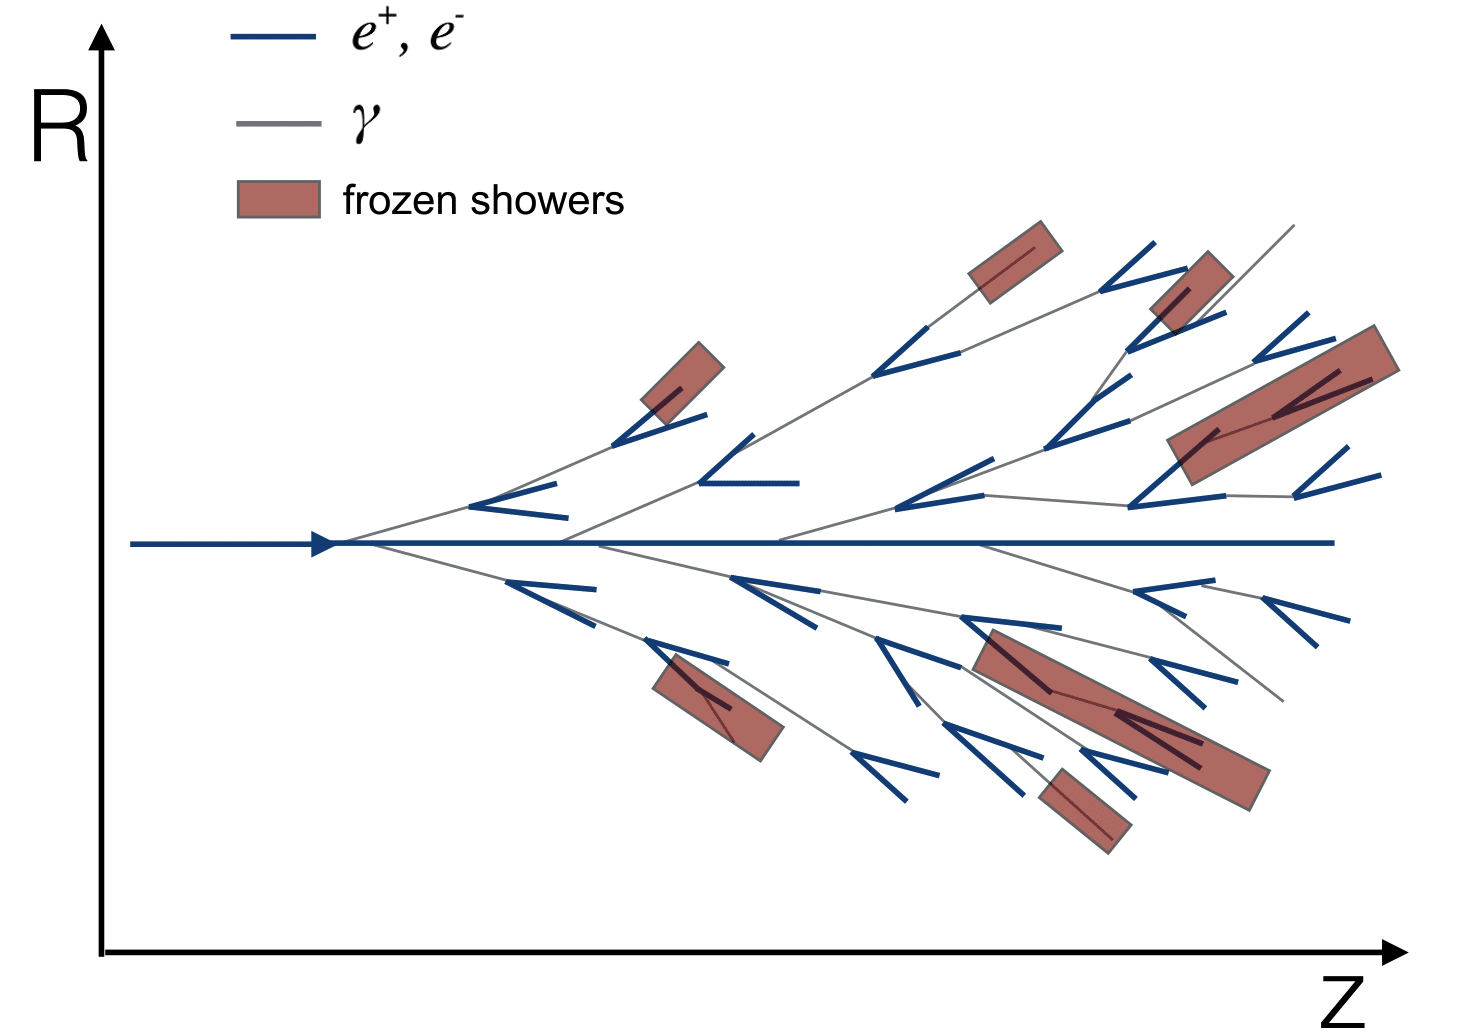
\includegraphics[width=0.9\textwidth]{MC/FSMethod2.png}
\caption{Diagram showing the shower substitution of the low-energy particle, during the high-energy particle simulation. Some of the showers from a particles, substituted by frozen showers method marked by a red squares}
\label{fig:MC_FS_method}
}
\end{figure}



\section{Introduction}\label{sec:FSproblem}




%\begin{figure}[!b]
%\center{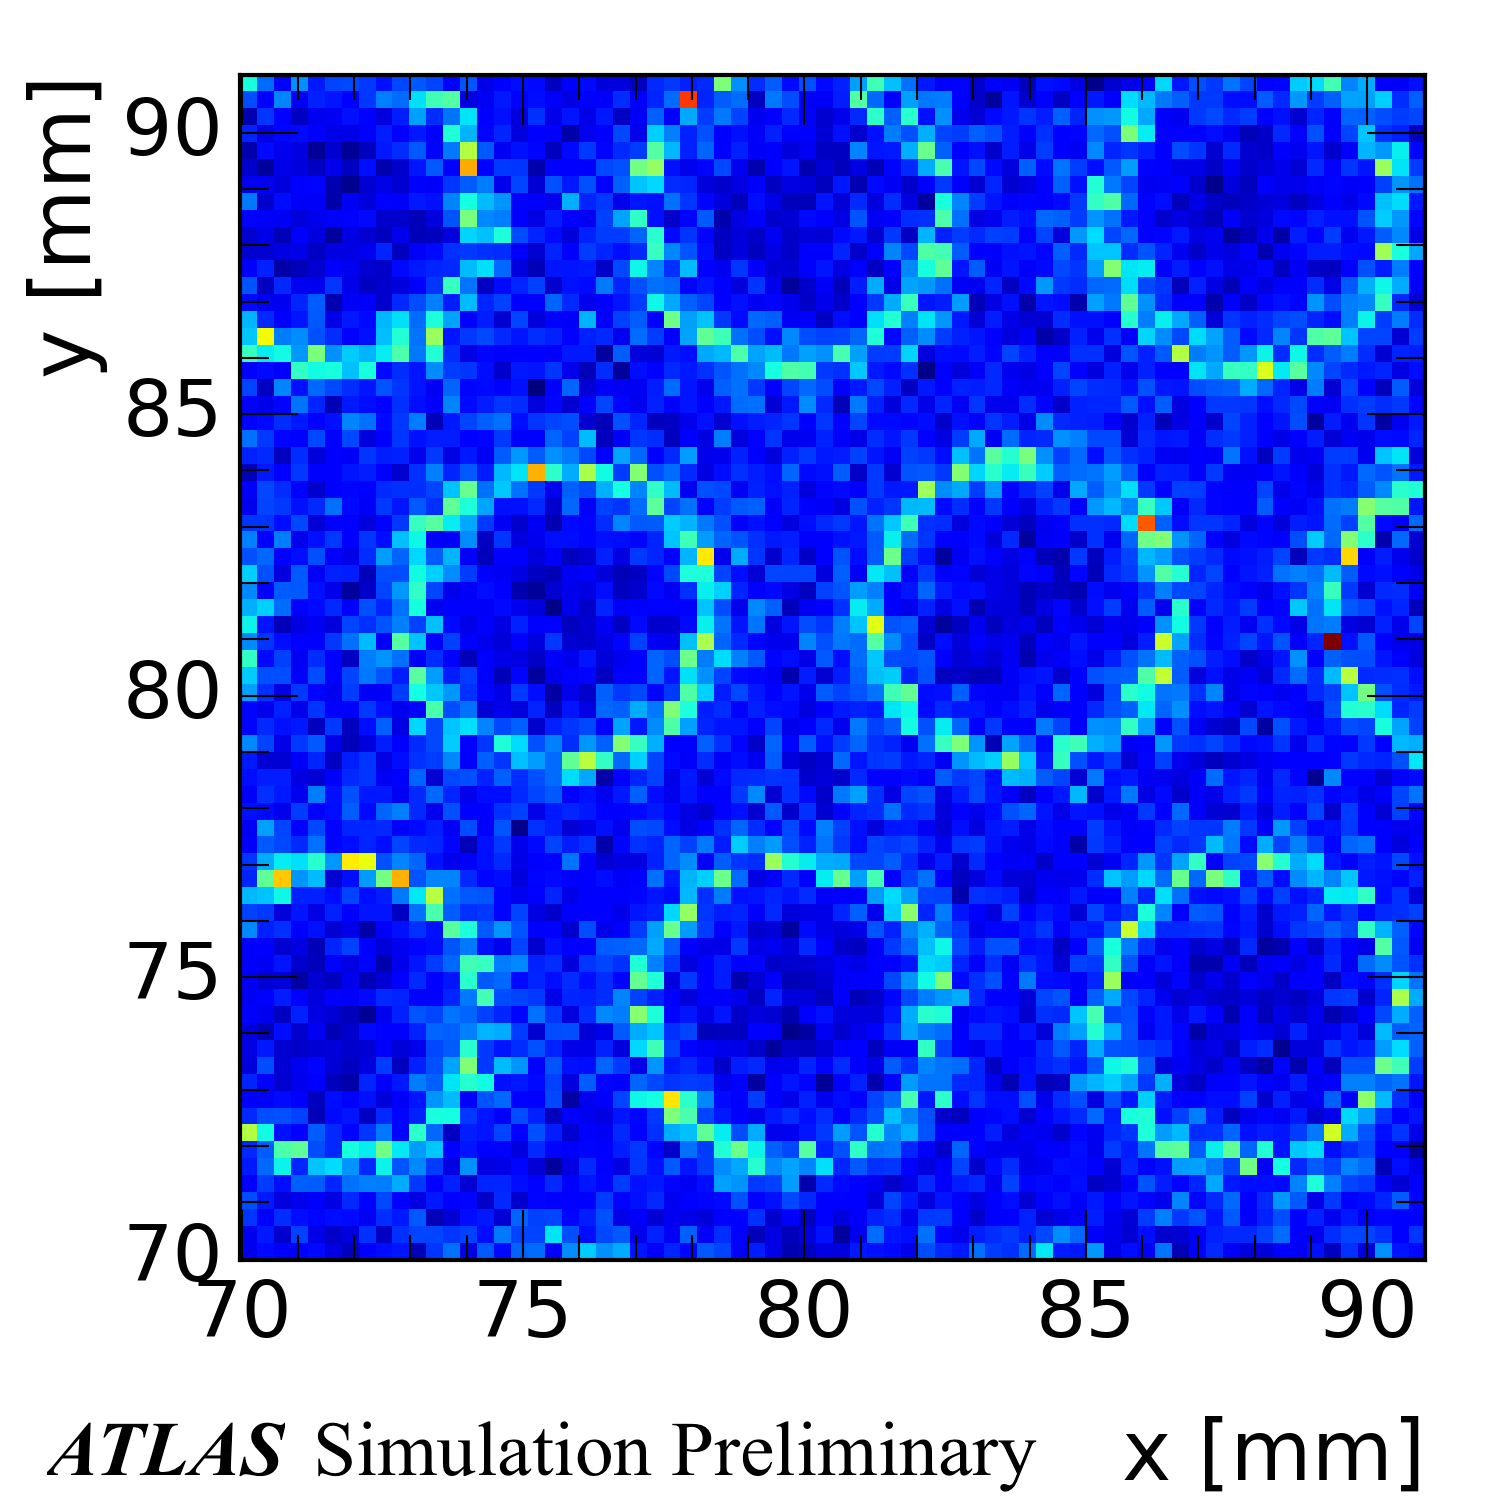
\includegraphics[width=0.5\linewidth]{MC/xySumE.png} }
%\caption{Shower energy response histogram in the x vs y plane for electrons, generated with uniformly distributed x and y and energy less than 1 GeV. Light circles are corresponding to a showers, started inside a LAr gaps with on average higher energy response, while the dark parts are corresponding to dead material respectively with smaller sum of the "hits" energy. }
%\label{fig:FSFluctuations}
%\end{figure}

\begin{figure}[!tbp]
\begin{minipage}[h]{0.49\linewidth}
\center{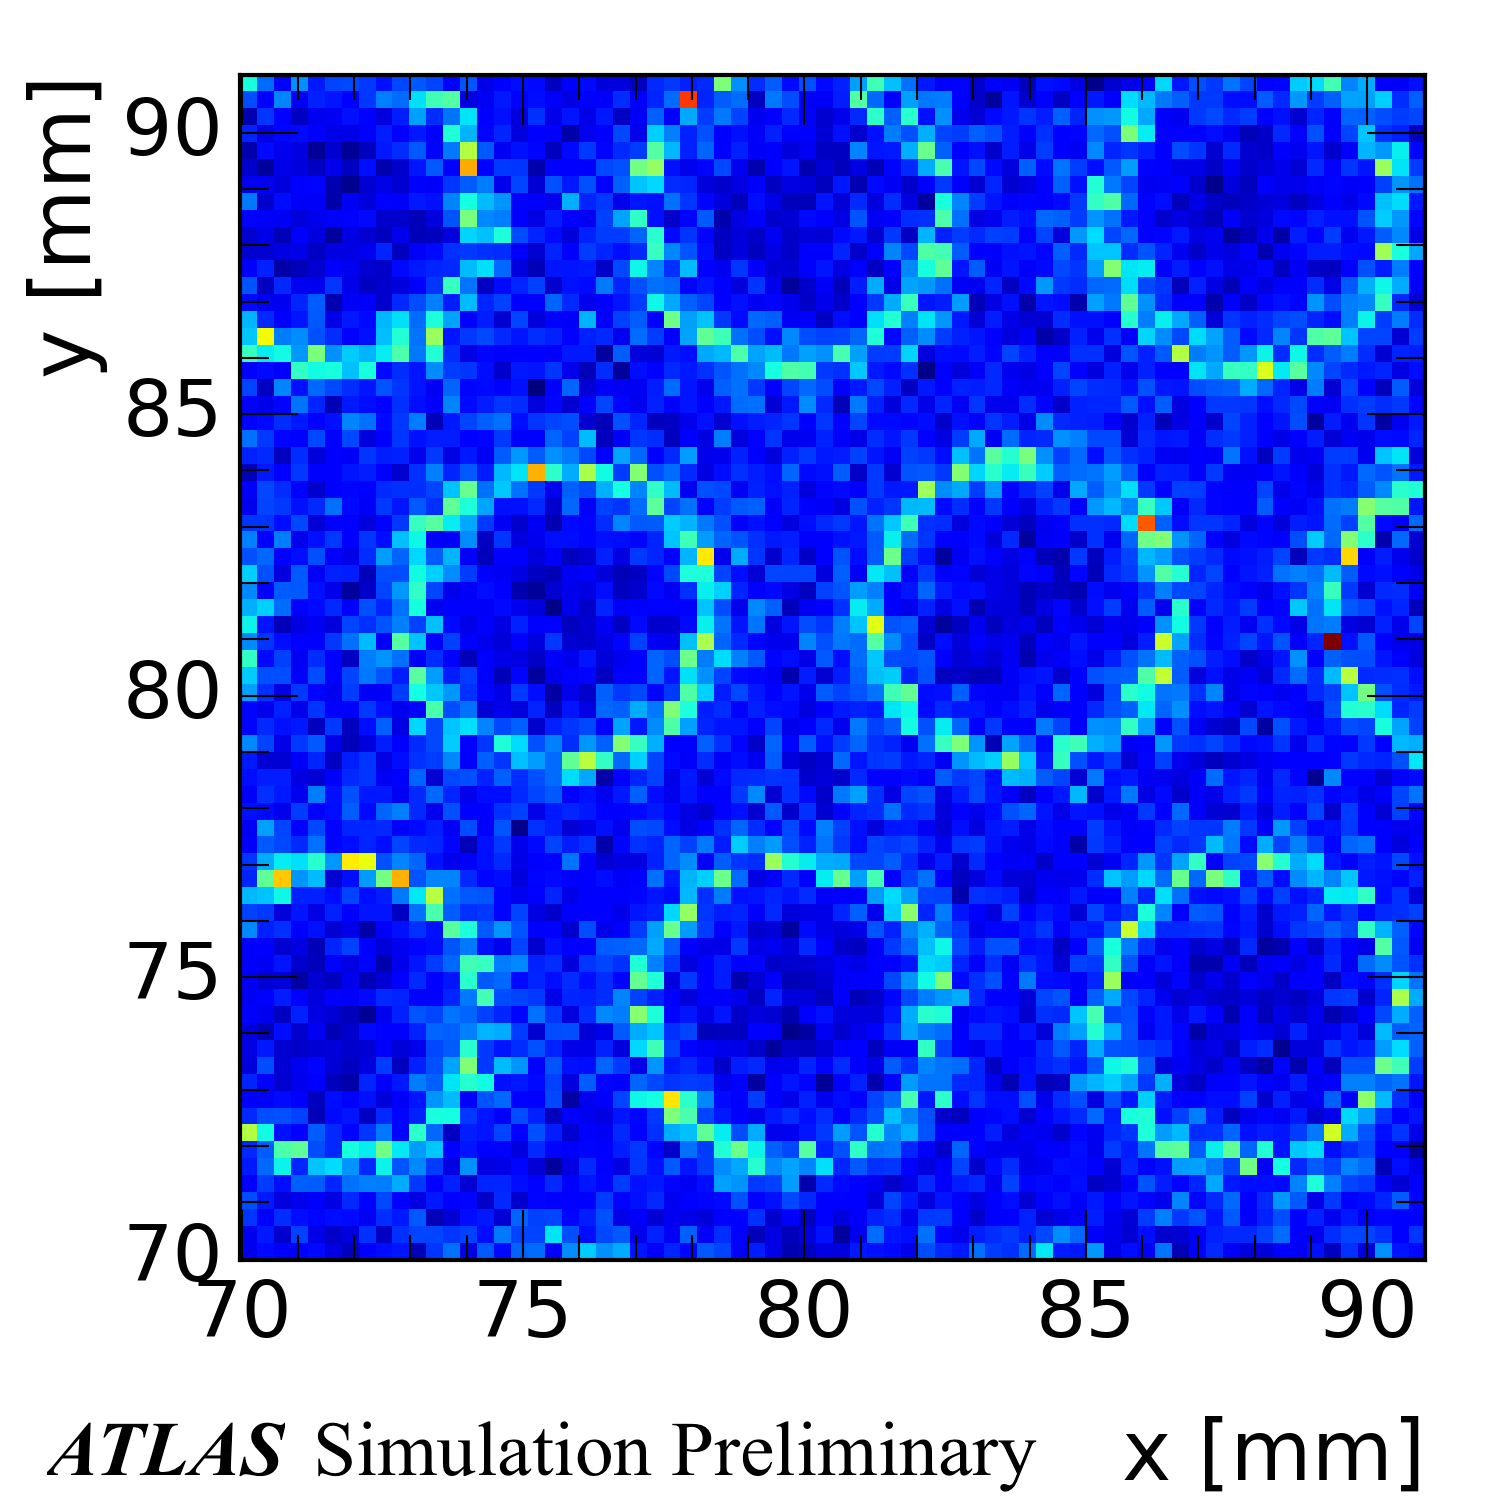
\includegraphics[width=0.9\linewidth]{MC/xySumE.png} \\ a)}
\end{minipage}
\hfill
\begin{minipage}[h]{0.49\linewidth}
\center{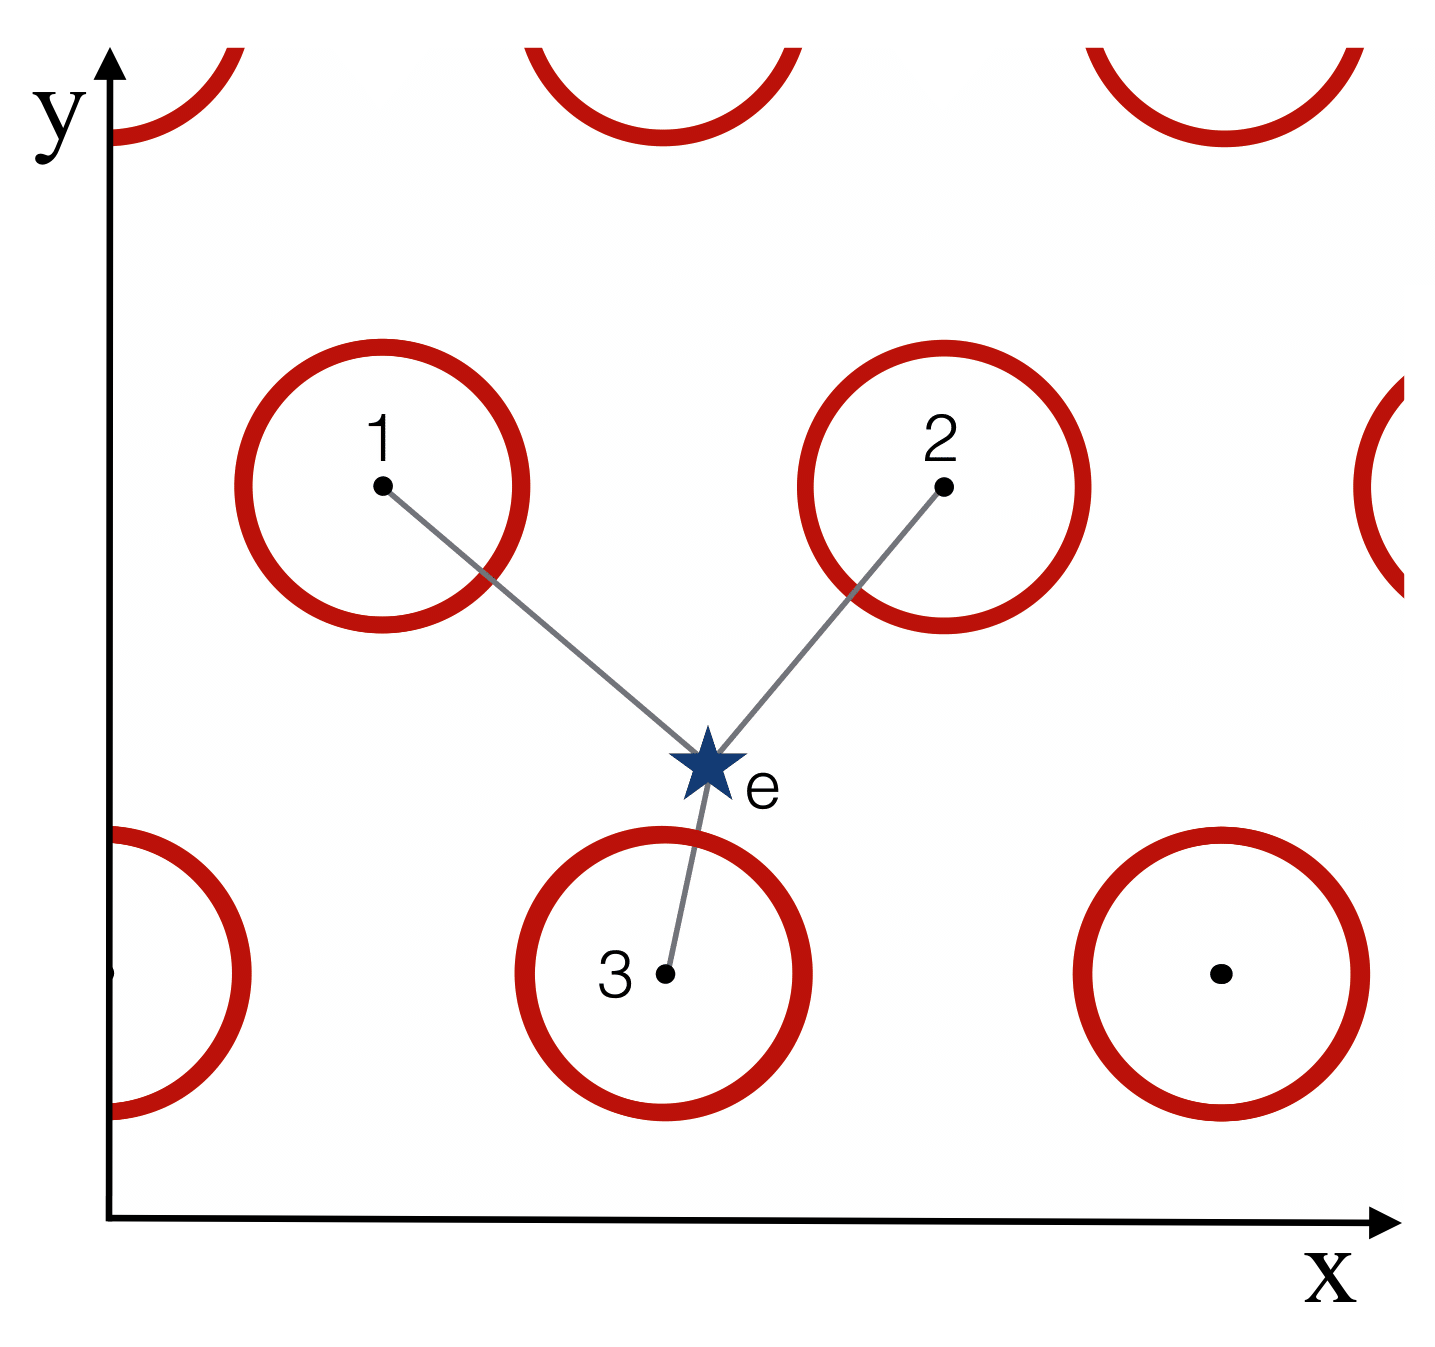
\includegraphics[width=0.9\linewidth]{MC/DistanceCalculation.png} \\b)}
\end{minipage}
\caption{ a) Shower energy response histogram in the x vs y plane for electrons, generated with uniformly distributed x and y and energy less than 1 GeV. Light circles correspond to showers, started inside LAr gaps with on average higher energy response, while the dark parts correspond to dead material with smaller sum of the "hits" energy.
b) Distance to a closest rod center scheme $d_{rod} = min( d(1,e), d(2, e), d(3, e))$, where 1,2,3 are the positions of the rod centers and e is the position of initial electron.. Rod centers and liquid argon gaps are shown by black and red circles respectively.}
%\caption{Distribution a) electron energies and b) mean number of hits in a shower vs energy of electron for electrons with energy less than 1 GeV coming from initial electron with energy 1 TeV. }
\label{fig:FSFluctuations}
\end{figure}


\begin{figure}[!tbp]
\begin{minipage}[h]{0.49\linewidth}
\center{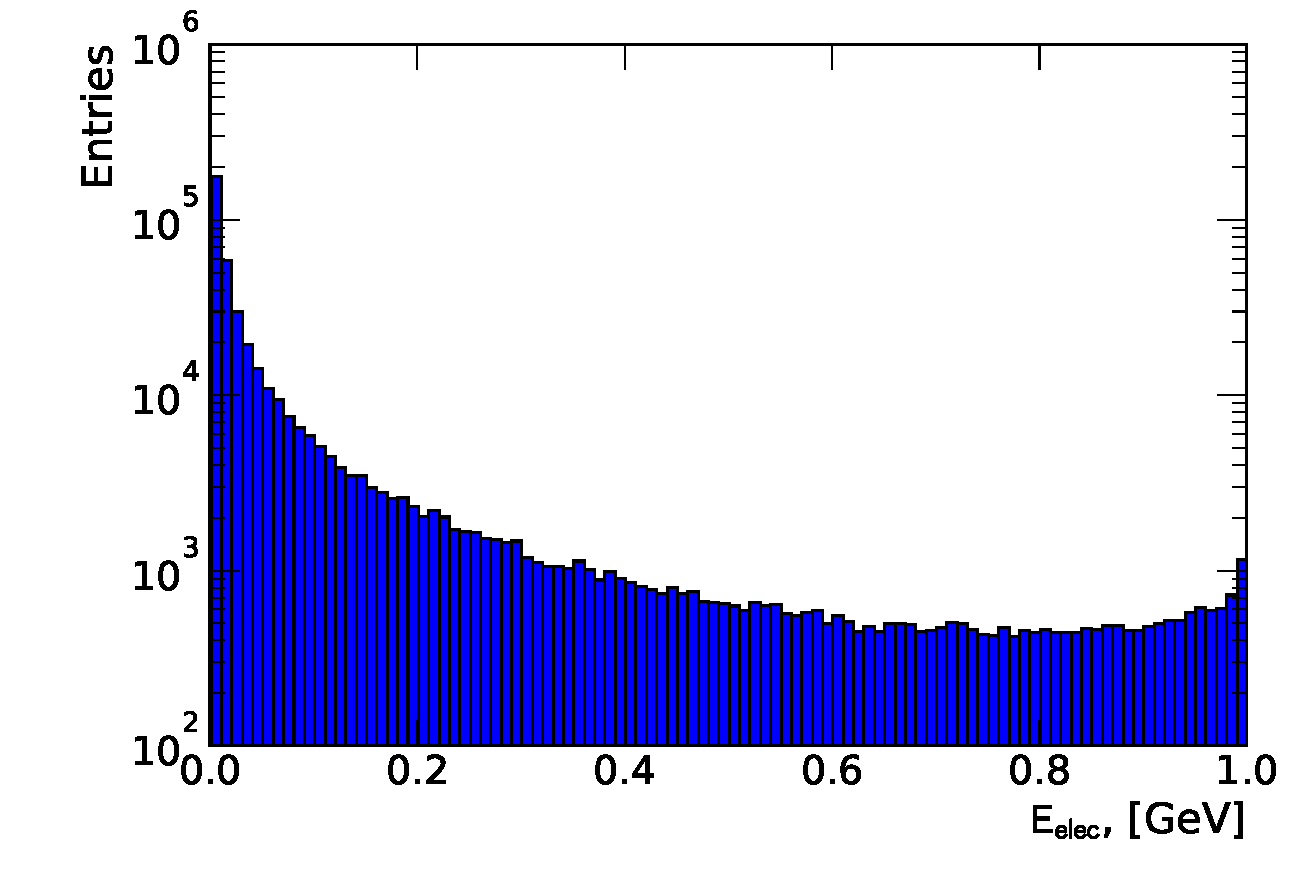
\includegraphics[width=1.0\linewidth]{MC/FSEnergy.pdf}  \\ a)}
\end{minipage}
\hfill
\begin{minipage}[h]{0.49\linewidth}
\center{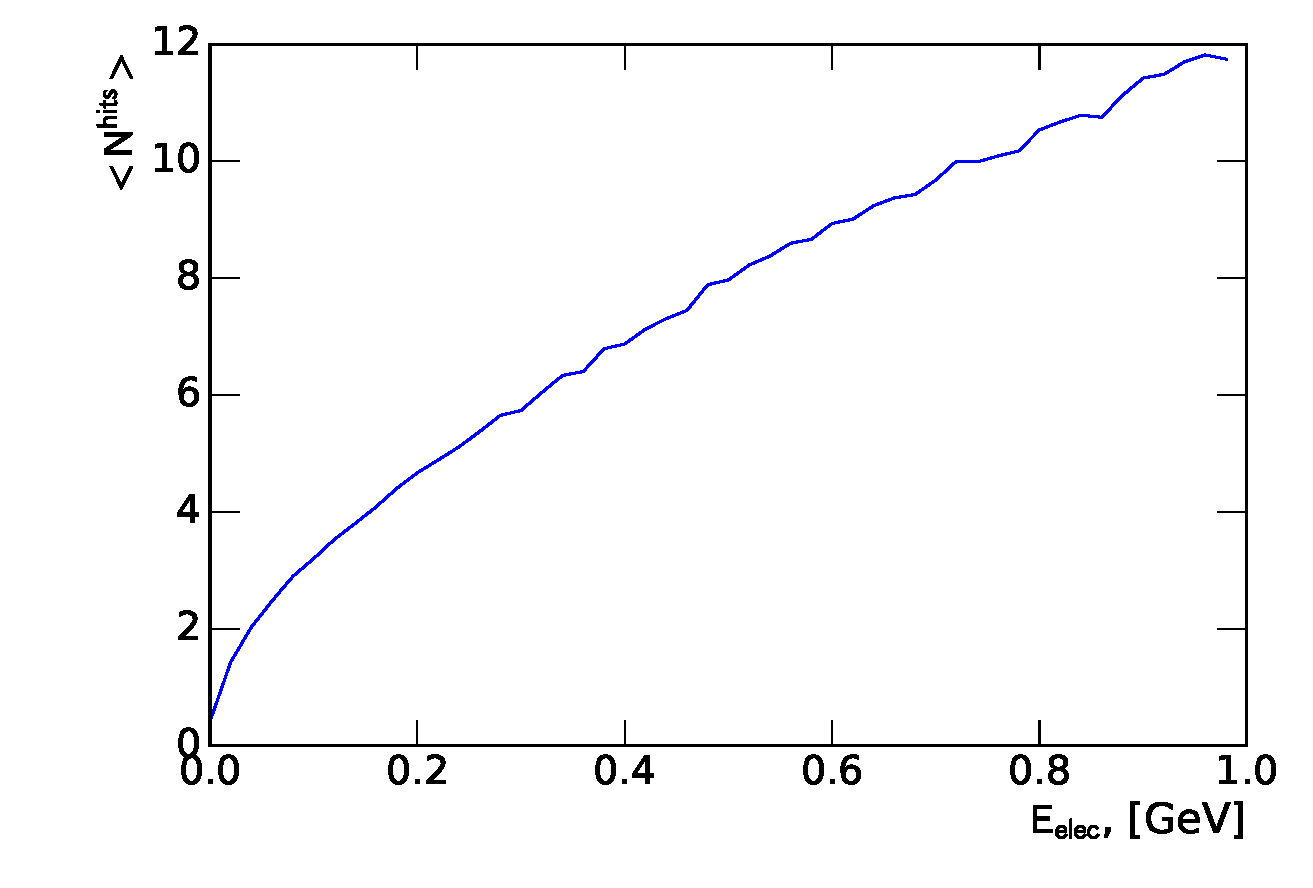
\includegraphics[width=1.0\linewidth]{MC/nHitsMean.pdf} \\ b)}
\end{minipage}
\caption{Distribution  of a) electron energies and b) mean number of hits in a shower vs energy of electron for electrons with energy less than 1 GeV coming from an initial electron with energy 1 TeV. }
\label{fig:TrackEnergy}
\end{figure}

The fast simulation of forward calorimeters (FCAL) is a complicated task due to its complex structure. As it was mentioned in Sec. ~\ref{sec:forwardCalo} FCAL consists of hexagonal absorber cells with anode tube and cathod rod in the cell center and liquid argon in the gap between rod and tube. In order to simulate the resolution of high energy electrons, good fast simulation technique should take into account this feature of a large amount of non-uniformly distributed sensitive material.

The energy resolution of an electron inside the calorimeter can be written as:
\begin{equation}\label{eq:EMResoultion}
\frac{\sigma}{E} \approx \frac{1}{\sqrt{E}}	\oplus \frac{1}{E} 	\oplus const,
\end{equation}
where symbol $\oplus$ indicates a quadratic sum. The first term is a 'stocastic term', which includes intrinsic shower fluctuations,the second  one takes into account readout noise effects and pile-up fluctuations. Constant term is connected to non-uniformities in a detector, causing large fluctuation of the energy loss. The energy resolution of high-energy electrons is mostly dominated by the constant term. 

Fluctuations due to the detector design are visible in a simulation of small energy electrons, generated at different points in forward calorimeter. Shower energy $E^{shower}$ distribution in the x vs y plane is showed on Fig. \ref{fig:FSFluctuations} a). The shower energy is defined as:
\begin{equation}
E^{shower}=\sum E_i^{hits},
\end{equation}
where $E_i^{hits}$ is an energy of i-th shower deposit inside the sensitive material. The periodic structure resembles the calorimeter design, where the light circles correspond to gaps with liquid argon. It could be reduced to a 1-d problem by introducing $d_{rod}$ distance to the closest rod center, calculated as shown on Fig. \ref{fig:FSFluctuations} b).

A typical electron substituted by a frozen shower coming from a simulation of high energy electrons has a relatively small energy (Fig. ~\ref{fig:TrackEnergy} a)). A mean number of depositions in a sensitive material in a "frozen" shower is around 5 and this value rises with electron energy (Fig. ~\ref{fig:TrackEnergy} b).  Fig. ~\ref{fig:FSProduction} presents the distribution of the distance to a closest rod center vs shower energy for showers from electrons with energy below 1 GeV coming from initial electrons with energy 1 TeV. The liquid argon gap is marked by red lines. There is a clear difference in showers energies between electrons born in a sensitive and dead materials. The differences in shower properties are also visible in a number of hits  (Fig. ~\ref{fig:ShowerProp} a) and the standard deviation of energy of the hits in the shower (Fig. ~\ref{fig:ShowerProp} b) distributions. The size of these differences depends on electron energies and higher for smaller energies (Fig. ~\ref{fig:FSProduction2} a) and less significant for higher energies (Fig. ~\ref{fig:FSProduction2} b).  This fact combined with energy distribution states an importance of a proper simulation of non-uniformities for showers coming from a small energy electrons.





\begin{figure}[!tbp]
\center{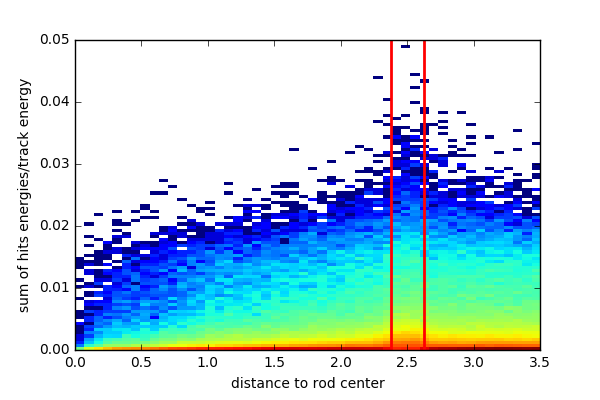
\includegraphics[width=1.\linewidth]{MC/fullBinningScatter.png} }
\caption{Distribution of distance to a closest rod center vs shower energy for electron showers created by electrons with energy less than 1 GeV coming from initial electron with energy 1 TeV in distance to a closest rod center vs shower energy plane. Position of a liquid argon gap is noted by a red lines. }
\label{fig:FSProduction}
\end{figure}

\begin{figure}[!tbp]
\begin{minipage}[h]{0.49\linewidth}
\center{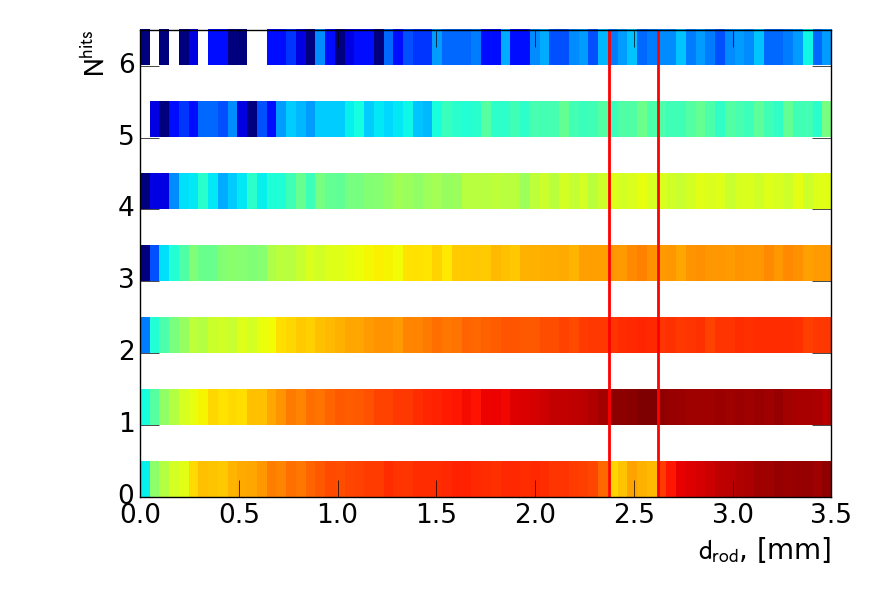
\includegraphics[width=1.0\linewidth]{MC/nHits.png}  \\ a)}
\end{minipage}
\hfill
\begin{minipage}[h]{0.49\linewidth}
\center{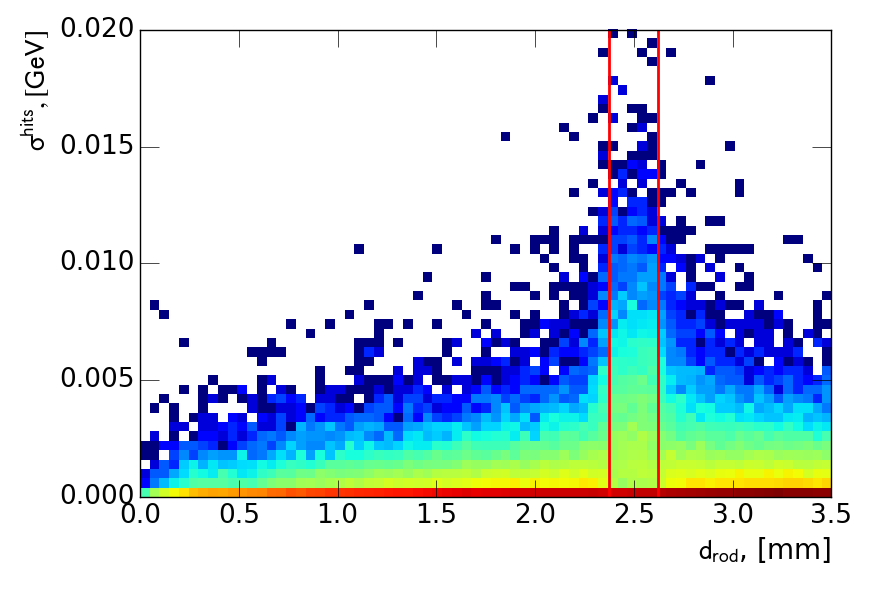
\includegraphics[width=1.0\linewidth]{MC/rms.png} \\ b)}
\end{minipage}
\caption{Distribution of distance to a closest rod center vs a) number of hits in a shower plane and b) standard deviation of hits in a shower energy of electron showers created by electrons with energy less than 1 GeV coming from initial electron with energy 1 TeV. Position of a liquid argon gap is noted by a red lines.}
\label{fig:ShowerProp}
\end{figure}

\begin{figure}[!tbp]
\begin{minipage}[h]{0.49\linewidth}
\center{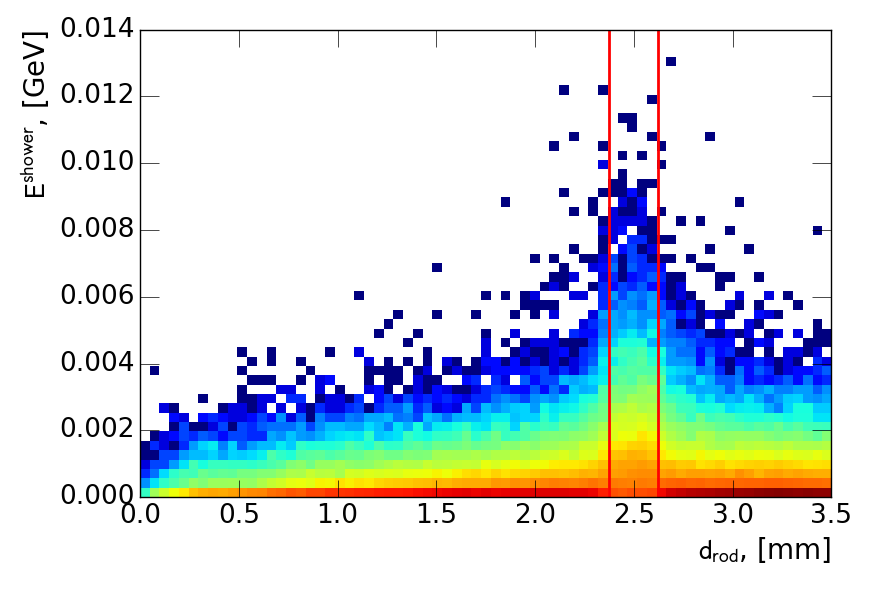
\includegraphics[width=1.\linewidth]{MC/fullBinningScatterSmall.png} \\ a)}
\end{minipage}
\hfill
\begin{minipage}[h]{0.49\linewidth}
\center{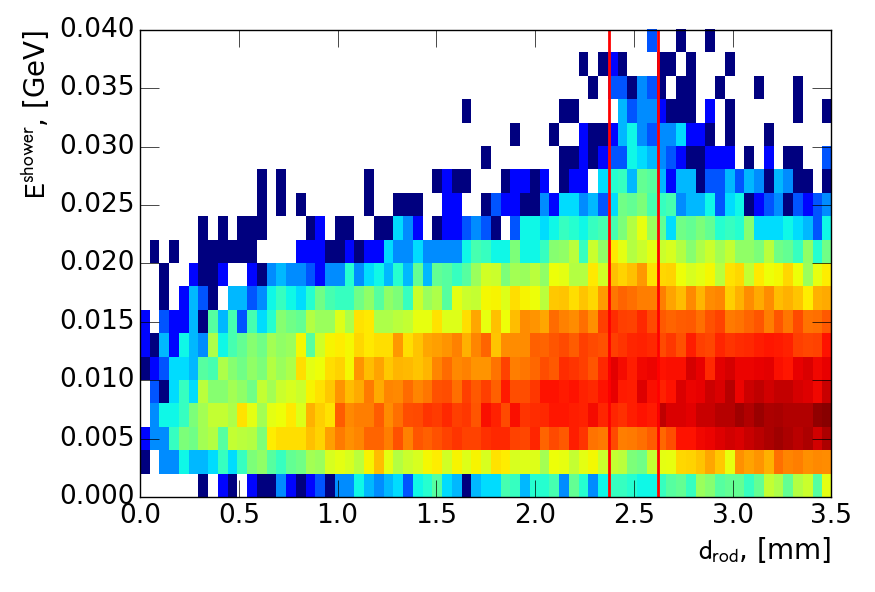
\includegraphics[width=1.\linewidth]{MC/fullBinningScatterBig.png} \\ b)}
\end{minipage}
\caption{Distribution of distance to a closest rod center vs shower energy for electron showers created by electrons with energy a) less than 100 MeV  and b) higher than 300 GeV coming from initial electron with energy 1 TeV in  plane. Position of a liquid argon gap is noted by red lines. }
\label{fig:FSProduction2}
\end{figure}

On another hand, the use of the frozen showers in a small energy region can be suboptimal because of the small number of energy depositions in a shower. For electrons with energy less than 30 MeV 90\% of the showers have zero depositions and just 0.5\% of showers have more than 1 hit (Fig.~\ref{fig:fracHits}). Below this energy single energy spot model has shown a better performance in simulation.

\begin{figure}[!tbp]
\begin{minipage}[h]{0.49\linewidth}
\center{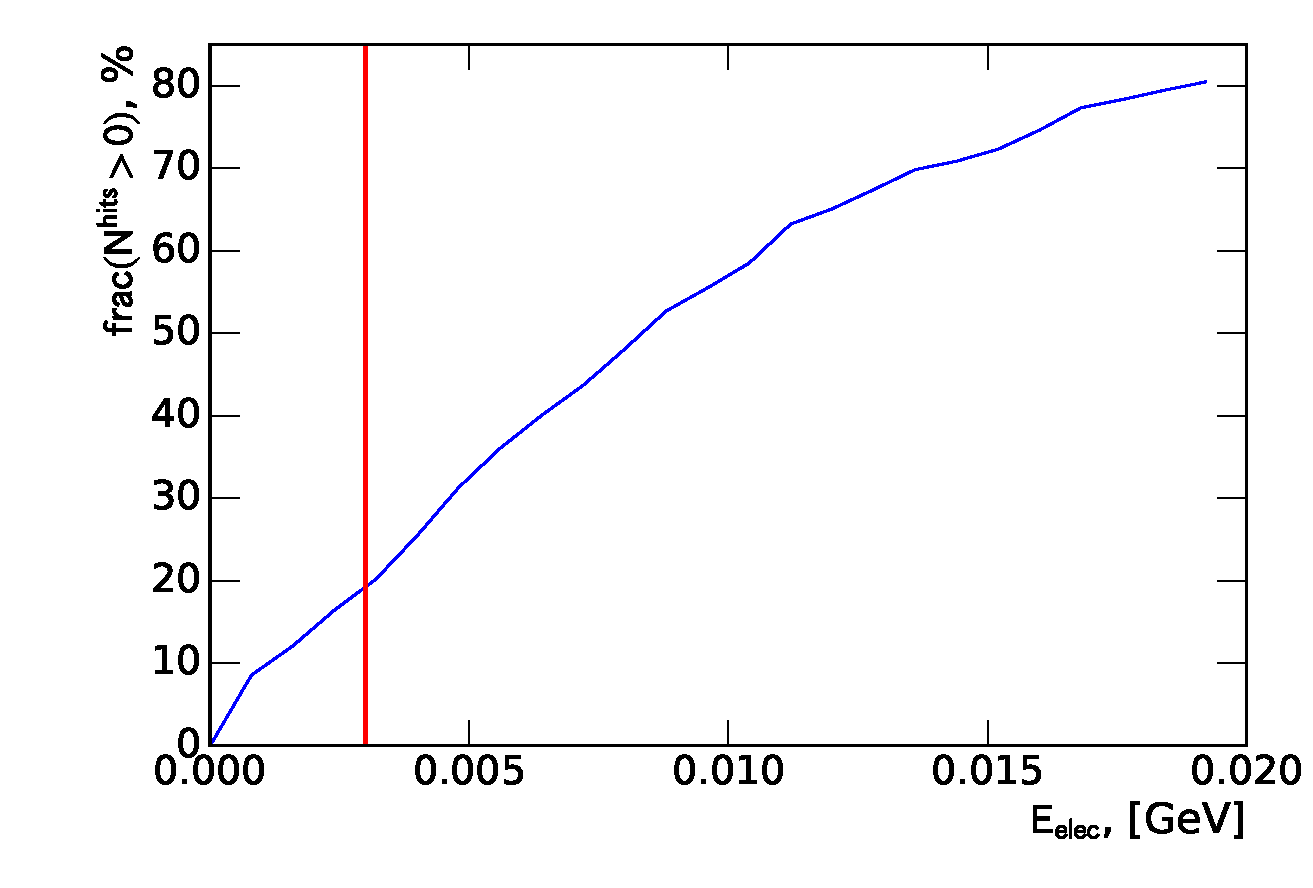
\includegraphics[width=1.\linewidth]{MC/fracHits2.pdf} \\ a)}
\end{minipage}
\hfill
\begin{minipage}[h]{0.49\linewidth}
\center{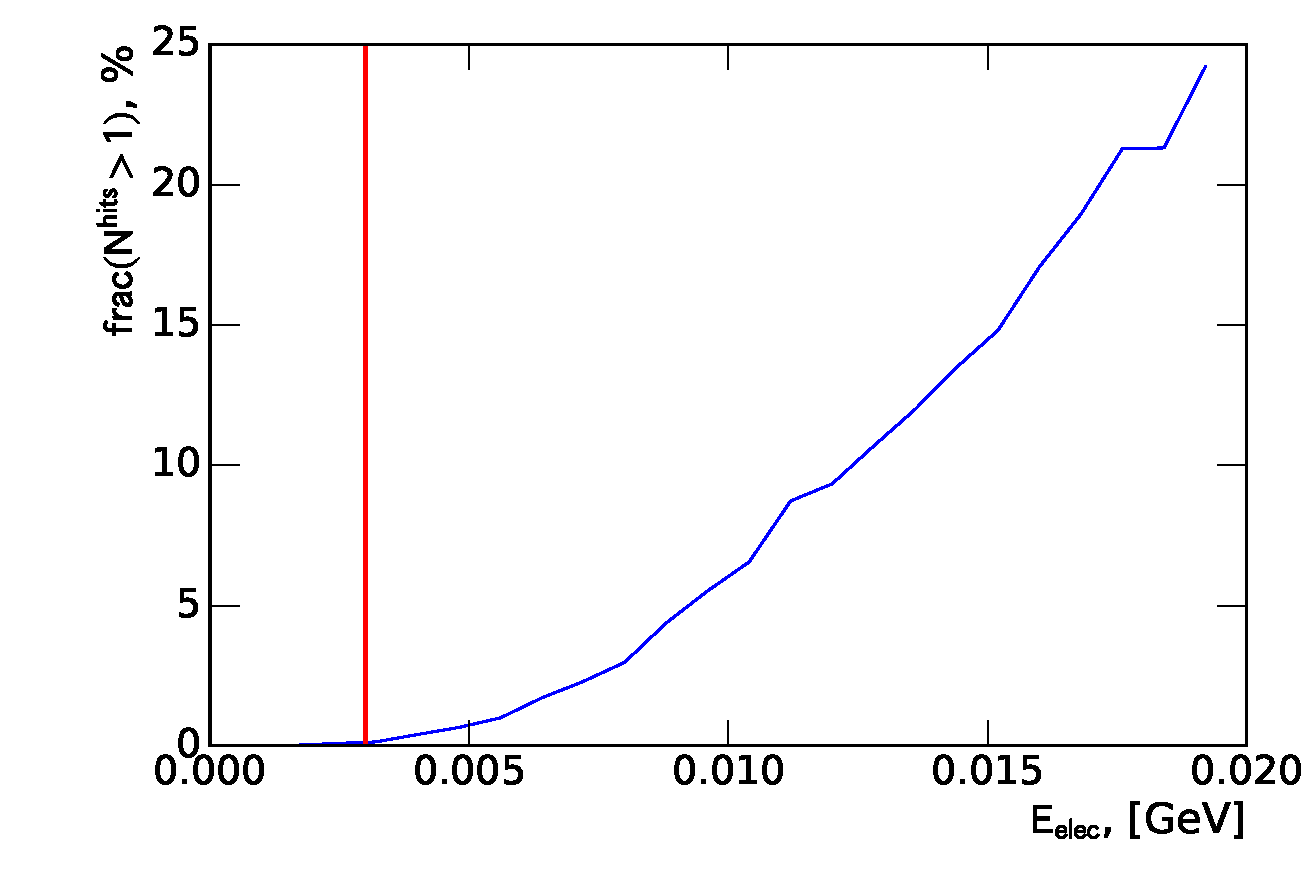
\includegraphics[width=1.\linewidth]{MC/fracHits.pdf} \\ b)}
\end{minipage}
\caption{Distribution of fraction of showers with a) at least 1 b) at least 2 depositions inside sensitive material depending on an initial electron energy. The red line denotes 30 MeV limit for a frozen showers method.}
\label{fig:fracHits}
\end{figure}


\section{Generation and use in simulation}

As it was mentioned in the introduction, the frozen showers method consist of 2 stages: generation of libraries and the use in simulation. Generation needs to be repeated for each significant change in the physics processes description in Geant4 or in a description of the detector. Showers are stored in a library in pseudorapidity and distance to a closest rod center bins, while energy remains unbinned. Distance binning was introduced to describe fluctuations from Sec. \ref{sec:FSproblem}. The position of the liquid argon gap bin corresponds to the real gap position. 

In order to have a proper energy distribution for generation of library particles coming from a simulation of physical process $t\bar{t}$ or high energy electrons are usually used. For each particle eligible for frozen showers use parameters are saved in a HepMC (reference) format for a later use. On a second stage, these particles are propagated through the calorimeter using standard \atlas simulation infrastructure. Each hit is saved as a shower inside library in a corresponding pseudorapidity and distance bin. 

Additionally, in order to save disc space as well as a memory consumption, the hit information is compressed. This compression is done in two steps: 
\begin{description}
\item [Hit merging] If the distance between any two hits is smaller, than a given parameter $R_{min}$, then hits are merged into one deposit at the energy weighted center of them. This process is done iterativelly.
\item [Truncation] Hits which energies are below the fraction f of the total energy sum of all hits, are truncated. The energy of remaining hits is rescaled back to preserve the total deposited energy.
\end{description}

During simulation, if an energy of a particle falls below a cut-off energy, the particle algorithm examines resulting shower containment. It checks whether  that particle is far from the edges of the calorimeter, so that the  shower is by 90\% inside the calorimeter. This depends also on an energy of the particle, because shower sizes are growing with energy. The algorithm searches for a shower with the closes energy in a corresponding pseudorapidity and distance bins. Shower is rotated in the direction of the particle. In order to correct the differences in the energy, each hit in a shower is scaled as:
\begin{equation}
E_{hit}^{new}=E_{hit}\cdot \frac{E_{part}}{E_{part,lib}},
\end{equation}
where $E_{hit}$ is the energy of the hit, $E_{part}$ is the energy of the particle and $E_{part,lib}$ is the energy of the particle from a library. Then particle is substituted by a resulting shower. Later, reconstruction algorithm uses hits from a frozen shower as a usual energy deposits in a sensitive material. 

\begin{figure}[!tbp]
\center{
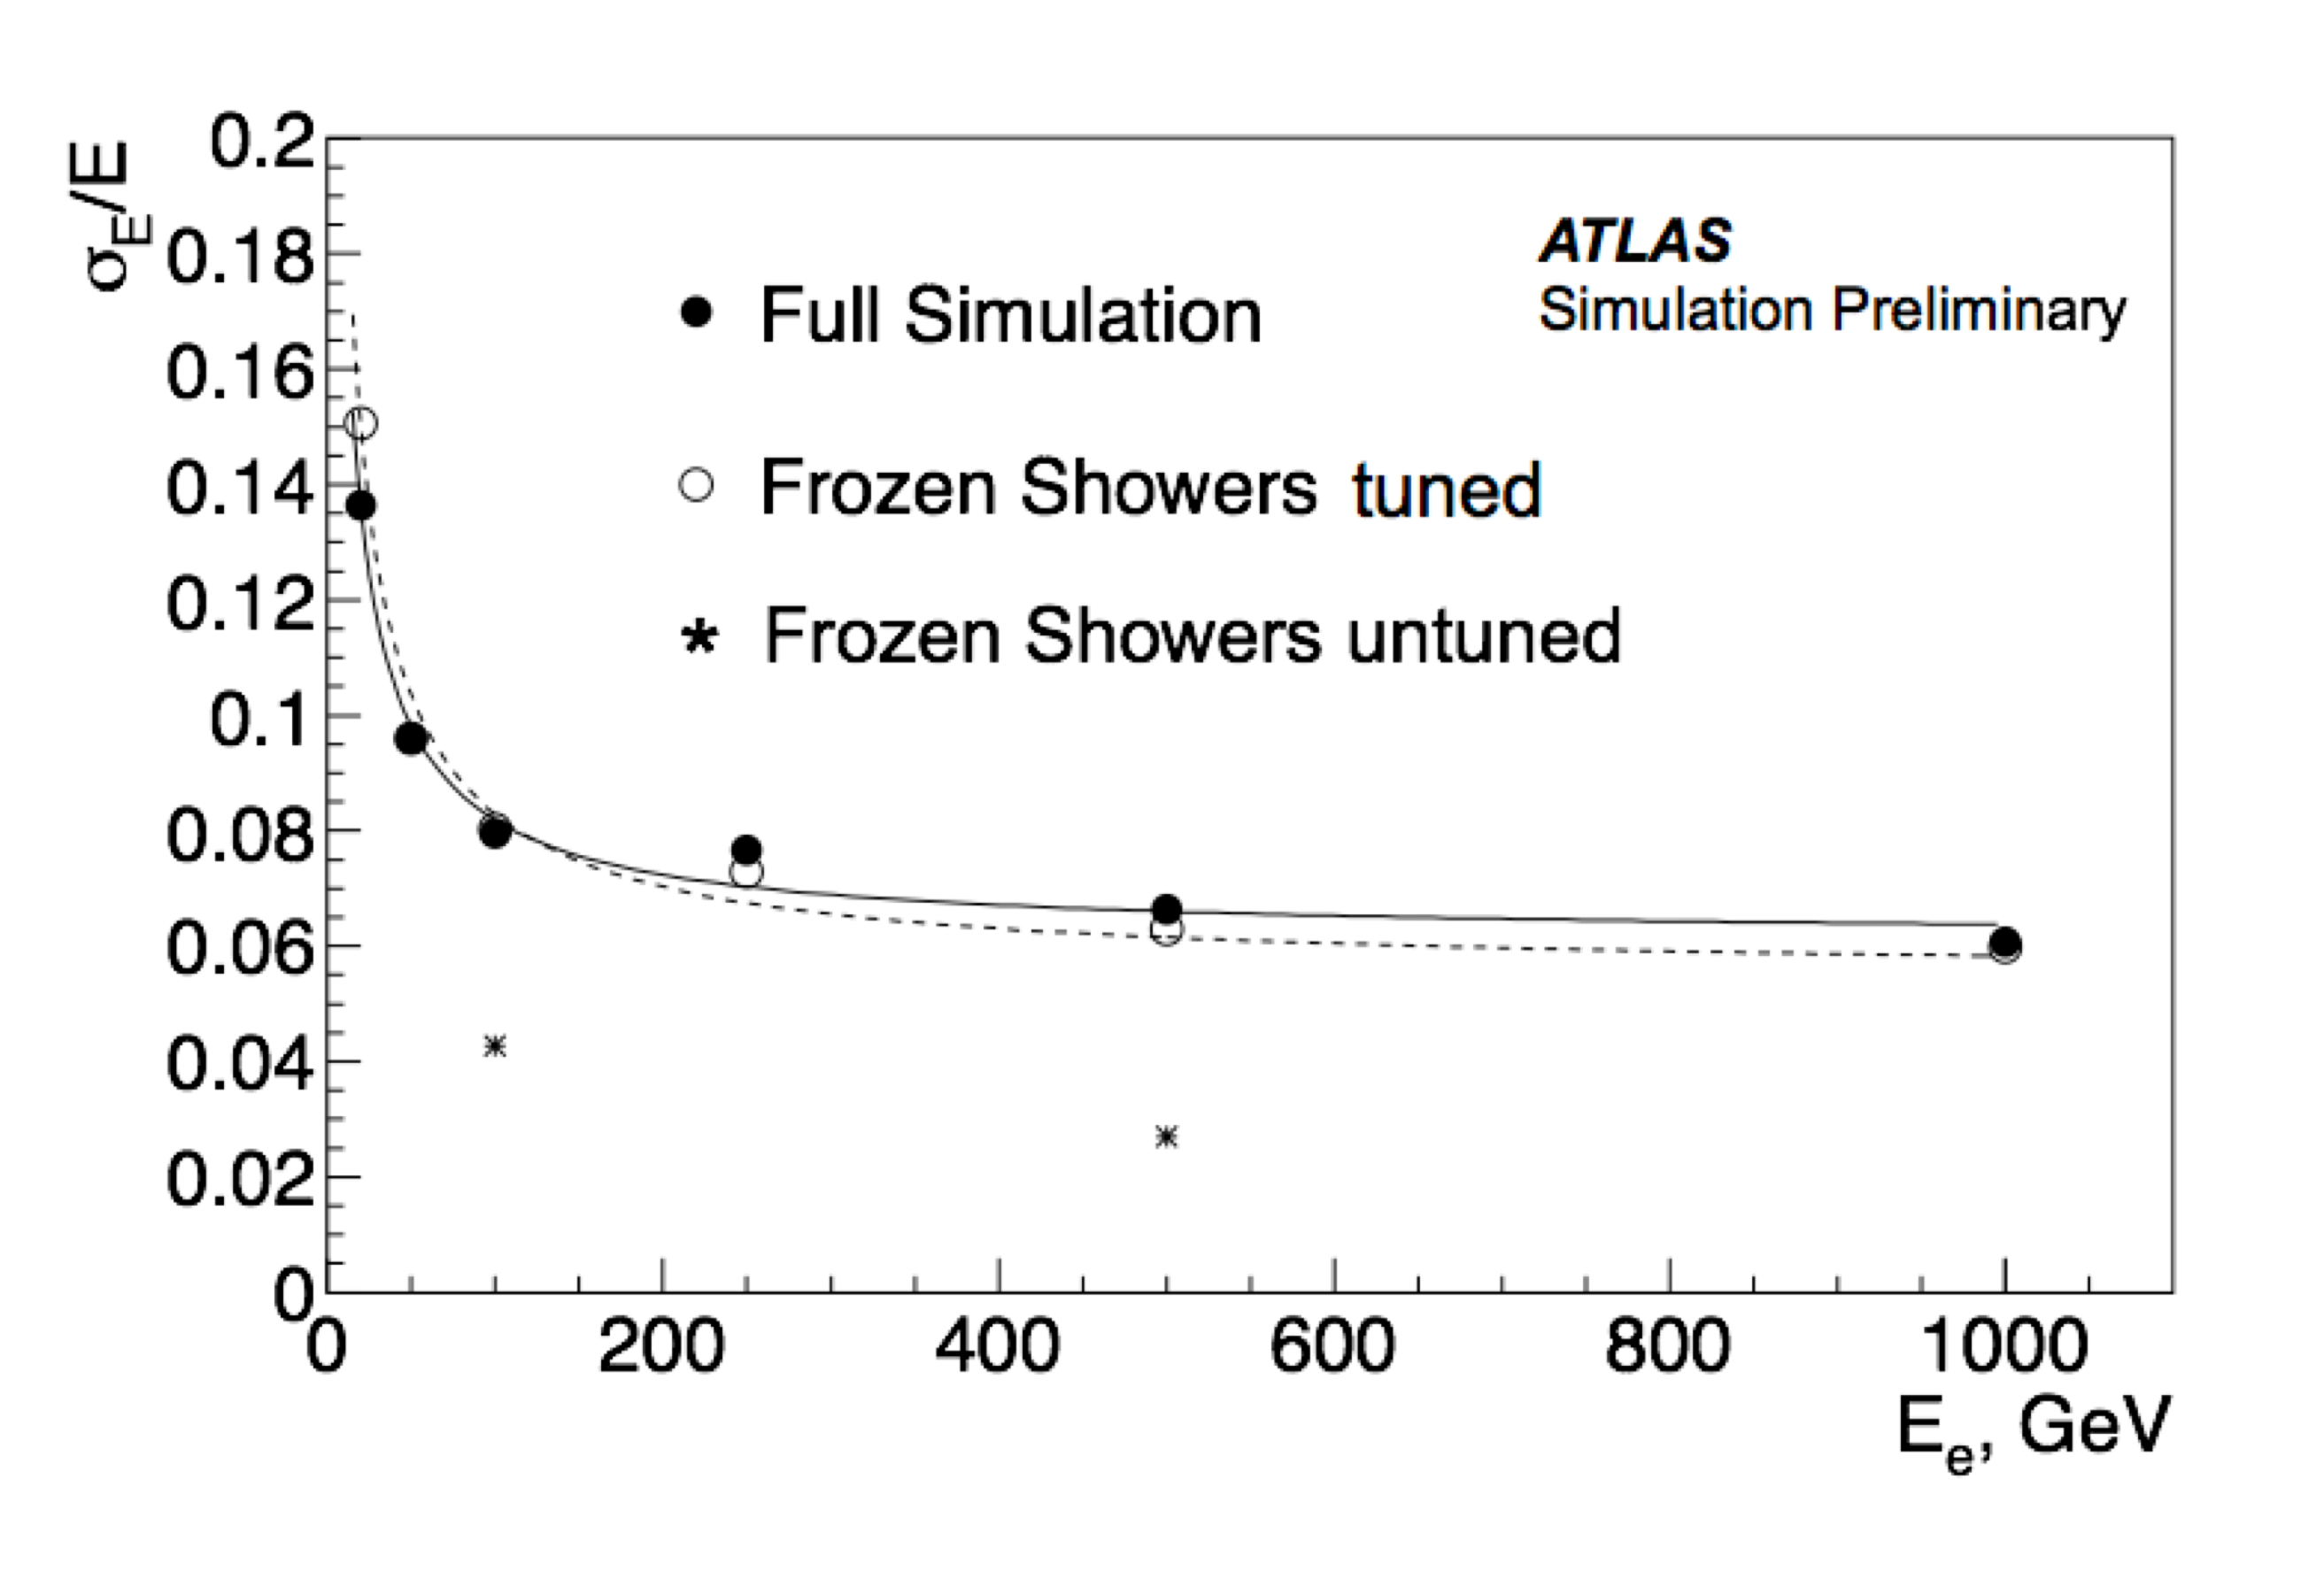
\includegraphics[width=0.8\textwidth]{MC/fs.png}
\caption{Electron resolutions for full simulation(black dots), tuned(white circles) and untuned(star points) frozen showers. Electrons simulated with frozen showers libraries before tuning have twice smaller resolution, than an electrons from full simulation. Tuning allows to gain better agreement with full simulation.}
\label{fig:FS_resolution}}
\end{figure}

\begin{figure}[!tbp]
\center{
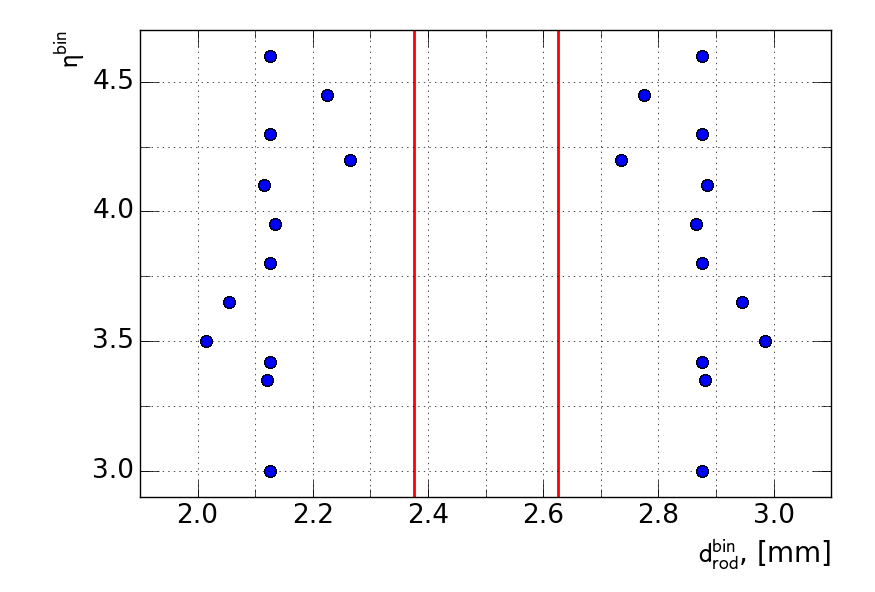
\includegraphics[width=0.8\textwidth]{MC/oldTuning.png}
\caption{Position of gap bins for different $\eta$ bins in old libraries after tuning. Dots are corresponding to a limits of each bin. Red lines are denoting original position of bins, that are corresponding to a position of a liquid argon gap in the calorimeter.}
\label{fig:FSOldTuning}}
\end{figure}

\subsection{Libraries tuning}\label{sec:LibTuning}

The good simulation method is required to be consistent with full simulation on all possible reconstucted objects. In case of Frozen Showers in forward calorimeter, the electron energy resolution is the most problematic value, since the resolution of the reconstructed electrons is around 2 times smaller(Fig.~\ref{fig:FS_resolution}), than in a full simulation. It may be caused by a lack of the showers from liquid argon gap in a simulation. Most of this effect is coming from the electron libraries. This means that these libraries require additional reconstruction-based tuning after generation.

Usual tuning consists of 2-step manual procedure:
\begin{description}
\item [Changing bin width] On this stage position of the liquid argon bin is moved, so what a bid width is enlarged. This causes a higher number of showers with higher responce in simulation and therefore higher size of fluctuations. This leads to a higher resolution and a mean energy of reconstructed electrons.
\item [Shower energy scaling] In order to correct for the shift introduced  in the mean energy, the shower energy is reduced by rescaling all the hits in a shower.
\end{description}
 It is repeated iterativelly in each pseudorapidity bin separately till the desired agreement is obtained. The resulting bin positions are shown on a Fig.~\ref{fig:FSOldTuning}. This method allows to have a relatively good agreement with full simulation (black dots on Fig.~\ref{fig:FS_resolution}). However, it is necessary to repeat this procedure for each new library generation and requires significant tuning effort, that makes it not optimal. 

\section{Machine learning based bin finding procedure}

Since frozen showers are planned to be used in Run-2 Monte-Carlo production, there is a need for a more automatic procedure of library generation with proper electrons resolution. One of the possible ways is to choose different position of liquid argon bin during libraries generation using machine learning tools. In this section automatic bin finding procedure will be discussed.
\subsection{Machine learning introduction} 

Machine learning is a set of algorithms, which allows computers to learn and give predictions without being specifically programmed. This is a modern field of computer science, that is wildly used in different fields like computer vision, natural language processing, data science etc. There are two main types of machine learning algorithms: supervised, where example of desired output is given by the "teacher" and the goal is to learn a general rule, that maps inputs to outputs and unsupervised learning, where no labels are given to the algorithm, and the algorithm discovers hidden patterns in the data. Initial data parameters of interest, that are used in algorithm to learn are called features. 

Machine learning algorithms can be used for solving a classification problem, where each event should be identified to one of the specified classes. Since the first introduction of the machine learning classifiyng algorithms called perceptron by Rosenblatt <ref> many different algorithms have been invented. In this analysis decision trees and support vector machines implemented in Scikit-Learn python package <reference> have been used. 

\subsubsection{Binary decision trees}

Binary decision trees, called also single decision trees, are one of the most commonly used machine learning algorithms for a classification problems in particle physics. It can be represented as a set of sequential cuts on input variables. 
Scheme of this algorithm is shown in Fig.~\ref{fig:MLAlgo} a). Red circles show the nodes of the tree. Each node corresponds to the one of the internal input variables and connected to two branches, that are split in the respect to the a variable. The first node is called a root node. Depth of the tree is a number of edges from the node to the tree's root node. The tree ends with squares, called leaf nodes, where all events are classified to a certain class. Leaf node represents classification or decision. The tree, where each node has at most 2 children called binary decision tree.

The tree is build using the variable called Shannon entropy, what is similar to the entropy in physics:
\begin{equation}
S=- \sum_{i=1}^{N} p_i log_2 p_i,
\end{equation}
where $p_i$ is the probability to find event of class i. Each split in a variable should decrease the entropy of the system. The information gain is defined as the difference in entropy after the split:
\begin{equation}
IG(Q) = S_0 - \sum_{i=1}^{2}S_i,
\end{equation}
where $S_0$ is the initial entropy, without new node, $S_i$ is the entropy of the one of the 2 node children. The node with the highest information gain is taken. One of the main advantages of the decision trees its simplicity of visualization and interpretation. 

\subsubsection{Support vector machines}

\begin{figure}[!tbp]
\begin{minipage}[h]{0.49\linewidth}
\center{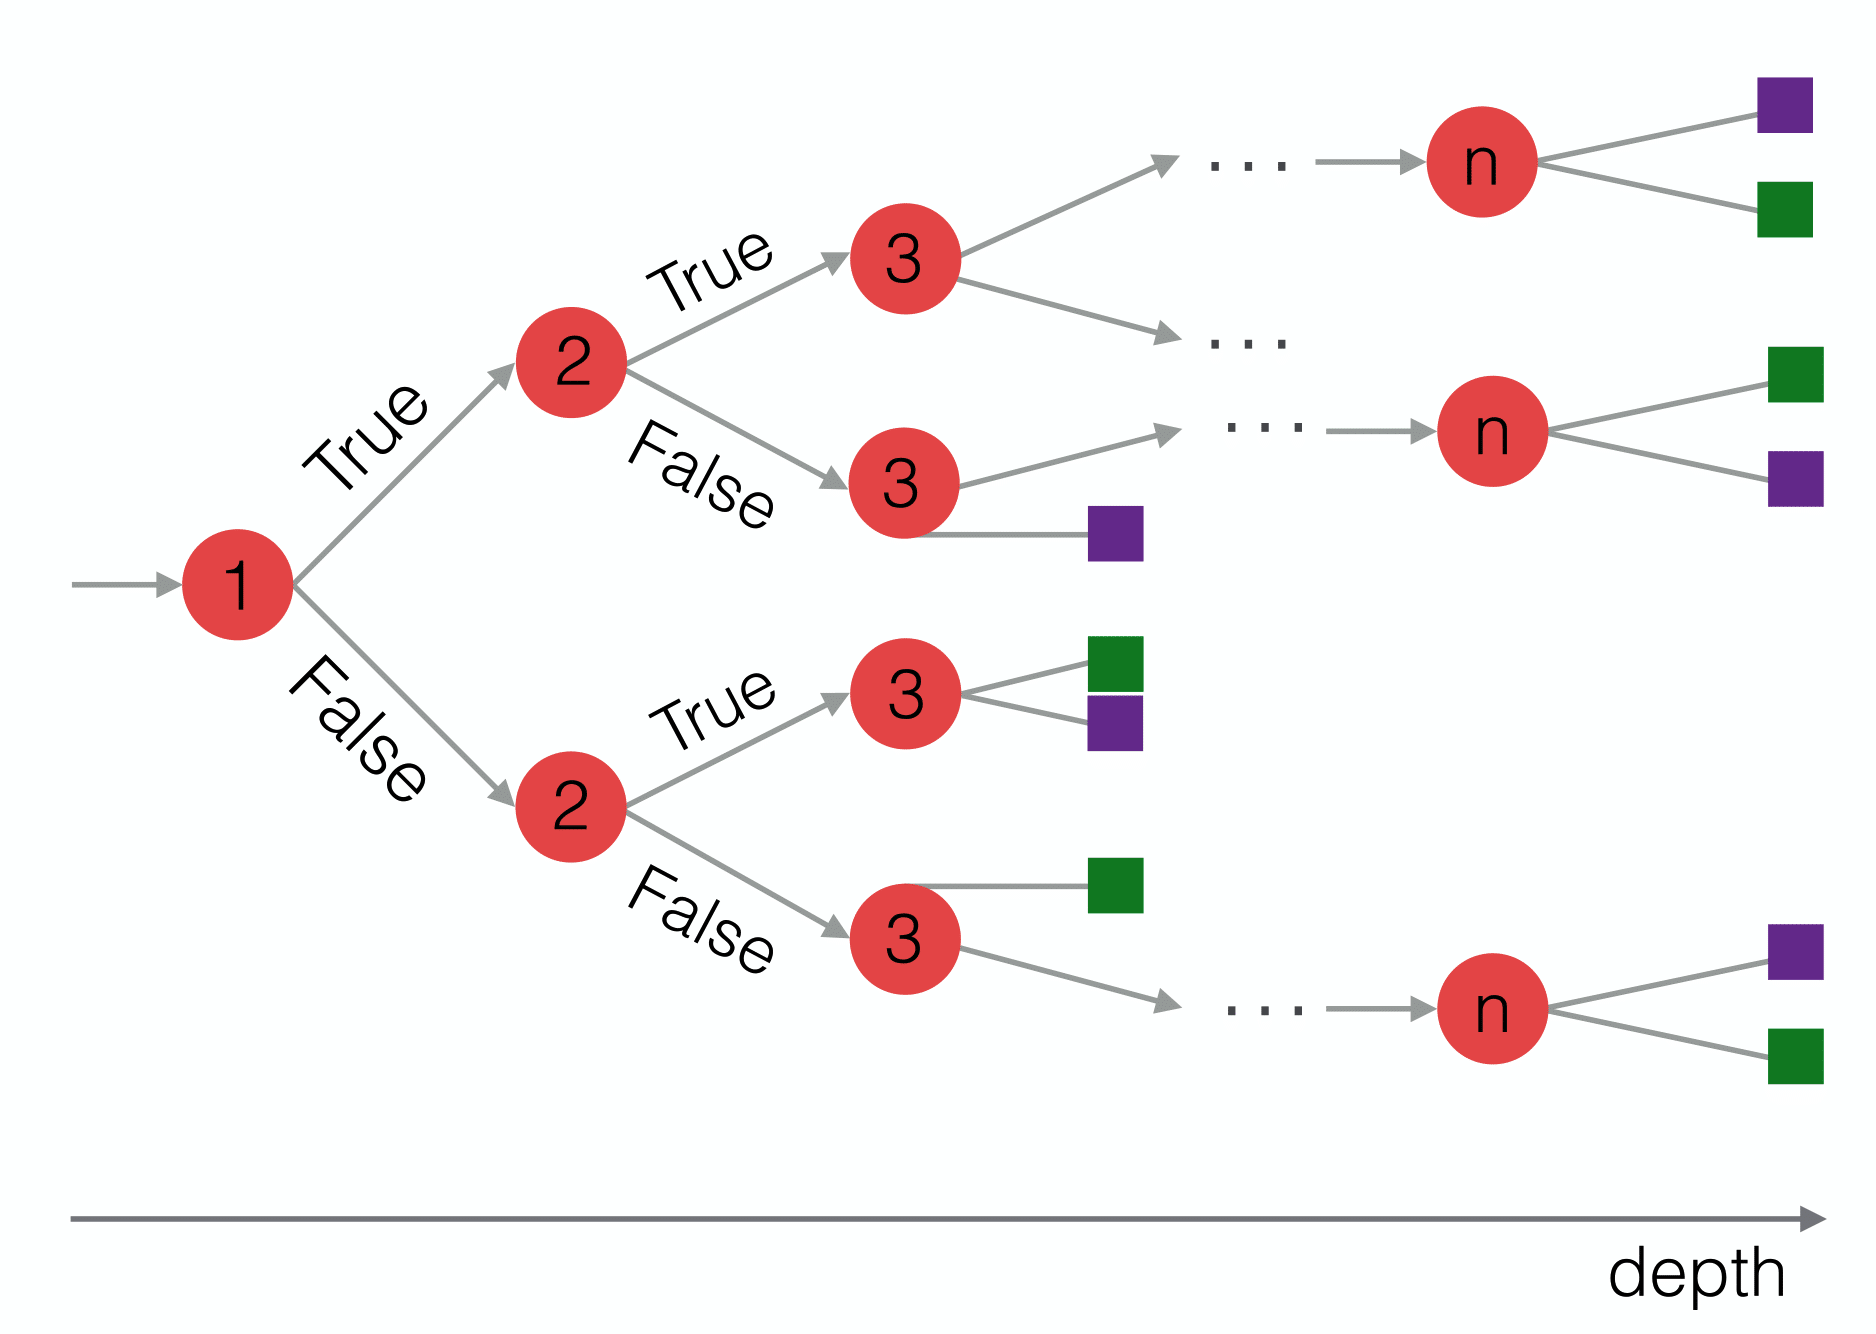
\includegraphics[width=1.\linewidth]{MC/DecisionTree.png} \\ a)}
\end{minipage}
\hfill
\begin{minipage}[h]{0.49\linewidth}
\center{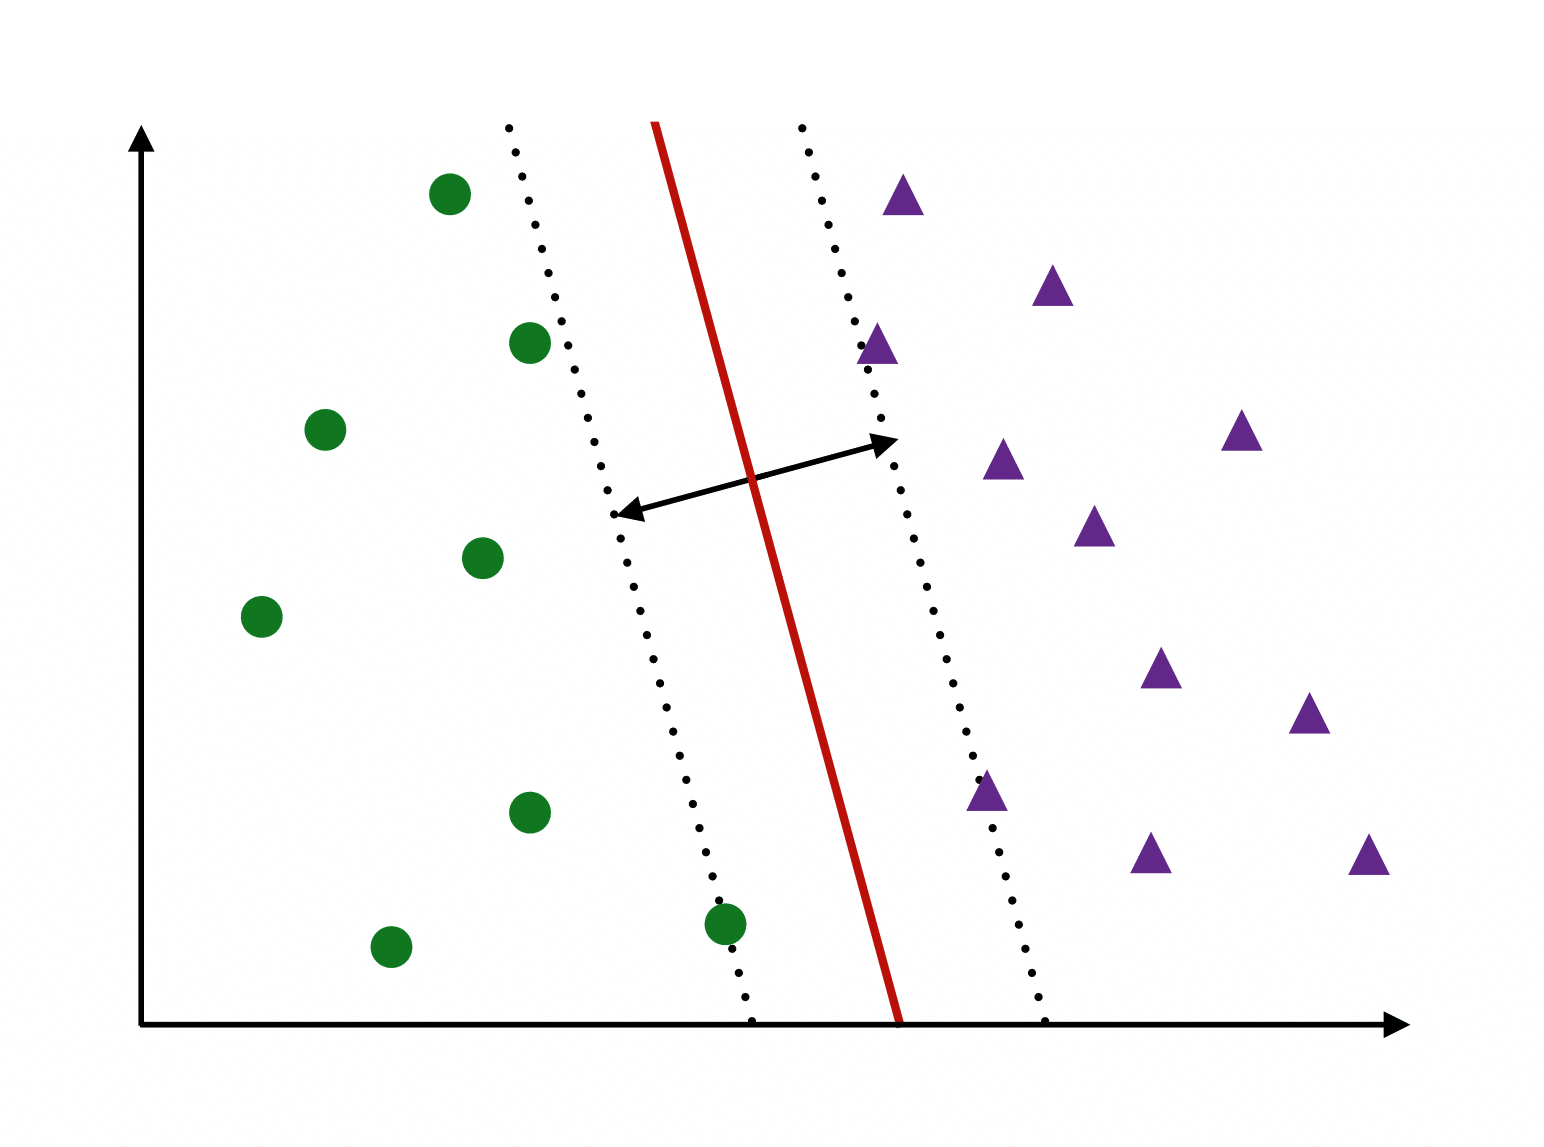
\includegraphics[width=1.\linewidth]{MC/SVM.png} \\ b)}
\end{minipage}
\caption{Schematic representation of machine learning algorithms, used in the analysis for a classification of showers. Green figures represent first class of events, whereas violet ones belong to a second class.  
a) Representation of a binary decision tree structure: red circles correspond to a nodes, that are split with the respect to the one of the features. Squares represent leafs, where events classified to a certain class. Depth of the tree is calculated as a maximum number of edges from the node or leaf to the root node. 
b) Representation of the SVM algorithm. Dividing hyperplane is shown by a solid line. The dashed lines represent the maximum margin boundaries}
\label{fig:MLAlgo}
\end{figure}

Support vector machines (SVM) is a supervised machine learning algorithm which can be used for classification problems. In this algorithm each event is represented in a p-dimensional parameter space. Classification is performed by finding a hyper-plane that differentiates given two classes with the largest possible separation (Fig. ~\ref{fig:MLAlgo} b). The hyperplane can be described with the set of points $\vec {x}$ in a parameter space satisfying:
\begin{equation}
\vec{w}\cdot \vec{x} - b = 0,
\end{equation}
where $\vec{w}$ is the normal vector to the hyperplane and the parameter $\frac {b}{\|{\vec {w}}\|}$ determines the offset of the hyperplane from the origin along the normal vector $\vec {w}$. 

The maximum margin boundaries are described by equations:
\begin{eqnarray}
\vec{w}\cdot \vec{x} - b = 1, \\
\vec{w}\cdot \vec{x} - b = -1,
\end{eqnarray}
where $\frac{2}{\|\vec{w}\|}$ is the distance between these 2 hyperplanes, so planes with the maximum margin between them should have the minimum $\|\vec{w}\|$. 

To prevent each point to fall into the margin, the following constrain should be satisfied: 
\begin{eqnarray}
\vec{w}\cdot \vec{x} - b \geqslant 1 \textrm{ where } y_i = 1,\\
\vec{w}\cdot \vec{x} - b \leqslant -1 \textrm{ where } y_i = -1,
\end{eqnarray}
where $y_i$ represents the class of the i-th event, that can be either 1 or -1. These equations can be rewritten as:
\begin{equation}
y_i(\vec{w}\cdot \vec{x} - b ) \geqslant 1
\end{equation}

It is also possible to construct a non-linear classifier by replacing the dot-product with a different \textit{kernel} function. In this thesis, a radial basis function (RBF) kernel is used:
\begin{equation}\label{eq:RBF}
K_{rbf}(\vec{x}_i, \vec{x}_j) = e^{-\gamma | \vec{x}_i - \vec{x}_j|^2} \, \gamma >0,
\end{equation}
where parameter $\gamma$ adjusts the width of the kernel.




\subsection{Model description}

\begin{figure}[!tbp]
\center{
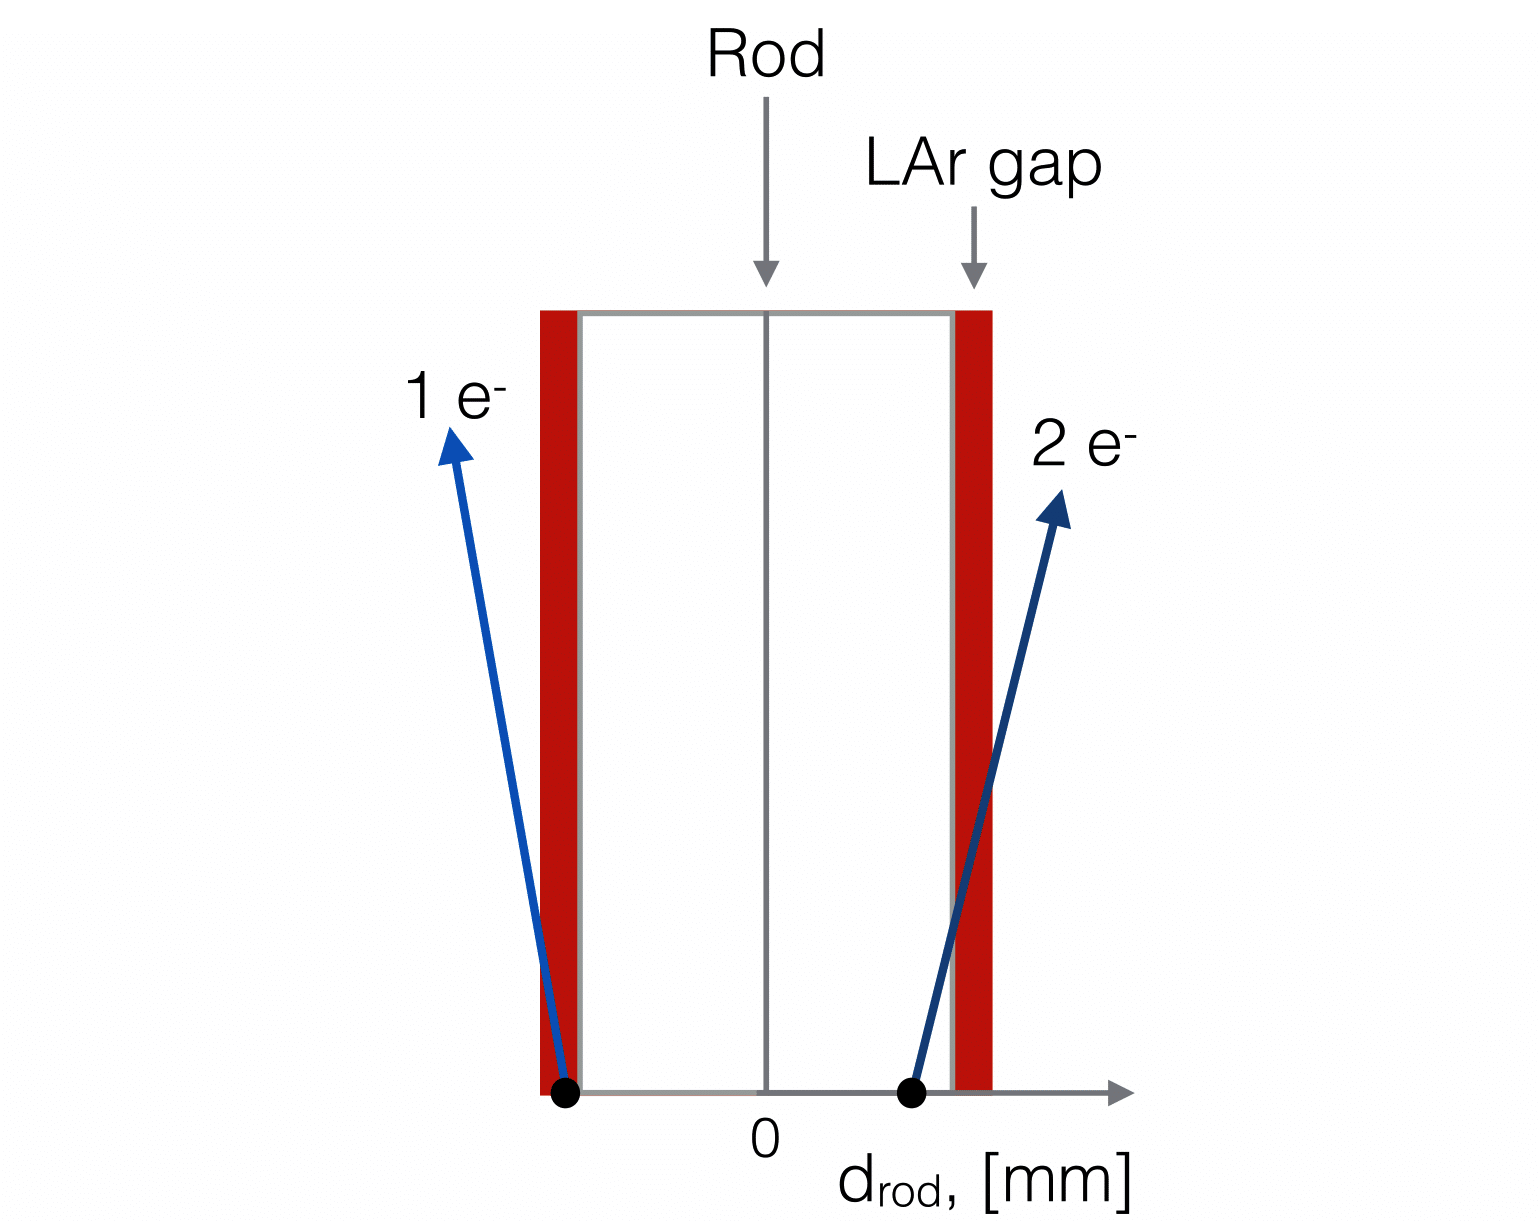
\includegraphics[width=0.5\textwidth]{MC/Model2.png}
\caption{Schematic representation of the model. Electron 1 is created in a liquid argon gap. Electron 2 is created near liquid argon gap and crosses it. This is causing a smearing of sensitive material showers distribution. Electrons created in a sensitive material tend to create more energetic showers, than electrons from a dead material. However, electrons, shown on this scheme, may give similar shower and therefore may not be distinguishable.}
\label{fig:Model}}
\end{figure}

As it was mentioned in a previous sections, modules in FCAL consist of different types of material and showers started inside the dead material are usually having smaller energies, than those started in sensitive material. However, the validation study (Fig.~\ref{fig:FS_resolution}) can be interpreted as an implication that there are high energy showers outside the liquid argon gap. It could be explained by the fact, that electron, created in a dead material, can cross a liquid argon gap and give a hit there as it is shown in Fig.~\ref{fig:Model} (electron 2). These electrons would be indistinguishable from electrons, created directly in a sensitive material (electron 1 in Fig. \ref{fig:Model}). 

It was decided to treat these electrons in the same way as electrons created in the sensitive material, and call the showers produced by them sensitive material showers. Showers that did not crossed a liquid argon gap, are called a dead material showers. This model leads to a bigger gap size from the definition.

From the definition, this model leads to the dependency of the liquid argon gap width on:
\begin{description}

\item [Electron energy] The gap should get wider with higher energy of the initial electron, because of the growth of the mean free path with energy.
\item [Direction of the electron] Electron aligned collinearly with liquid argon gap will have smaller probability to cross liquid argon gap. This probability will grow with the angle reaching its maximum at  $90^{\circ}$

\end{description}

\subsubsection{Training sample}

Real distributions, used in simulation, have a complicated structure and depend on a physics processes simulated. Machine learning could catch these dependencies, instead of the needed ones. This is why a simplified data is needed as a training sample for machine learning. The training sample was made by simulation of electrons, created in forward calorimeters. In order to treat equally high and low initial electron energy showers, the uniform distribution of energies is used.

Fig.~\ref{fig:EtaMomVsEnergy} shows the distribution of the shower direction ($\eta^{direction$) vs electron energy for electrons coming from simulation of 1 TeV electron. Most of the showers have direction in $\eta$ range between 3.0 and 5.0, that corresponds to position of the calorimeter. It was figured out, that the direction of the shower is highly correlated with the postion of the electron. Because of this it was decided to use electrons with direction, uniformly distributed between 3.0 and and 5.0.


\begin{figure}[!tbp]
\center{
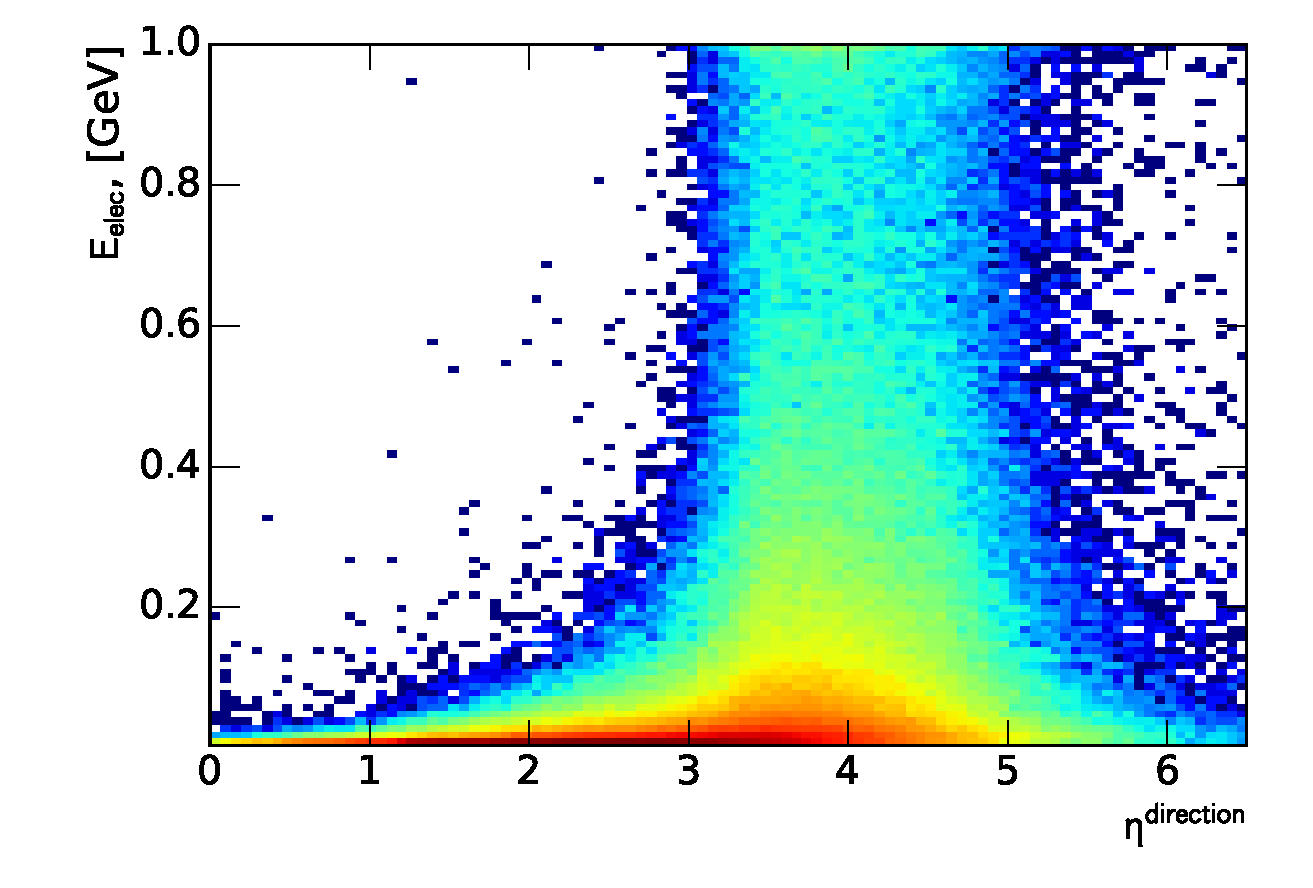
\includegraphics[width=0.8\textwidth]{MC/FSEtaMomVsEnergy.pdf}
\caption{Distribution of shower energy vs direction of shower $\eta_{momentum}$ for showers from the production of 1000 GeV electrons.}
\label{fig:EtaMomVsEnergy}}
\end{figure}

\subsubsection{First classifier}

The first classifier classifier aims to categorize all showers by means of shower parameters. It is possible to train supervised learning algorithm on pre-labeled artificially reduced training sample and then expand the classification to the full training sample. 

Pre-labeling could be easily done using a definitions of sensitive and dead material showers based on a distance to a closest rod center (Fig. \ref{fig:SchemePresel}). Showers started in a liquid argon gap are 100 \% sensitive material showers, while showers coming from electrons born near the rod center and on the edges of the the cells can be labeled as dead material showers, since there is a small probability for the electron, which caused the shower, to reach the liquid argon gap.

For this classifier it was decided to use simple decision trees, because it has shown good classification efficiency (around 97\%) on the reduced training sample. Different input parameters have been tested, and it was figured out, that the best set of the differentiating parameters is:

\begin{itemize}
\item Shower energy, that is equal to the sum of all sensitive material hits energies in shower;
\item Maximum hit fraction. This quantity is calculated as the energy of the most energetic hit divided by the shower energy;
\item RMS of the hits, calculated as a standard deviation of the hits energies in a shower.
\end{itemize}

Predictions of the first classifier for a full training sample is shown in Fig.~\ref{fig:Class} a). 

\begin{figure}[!tbp]
\center{
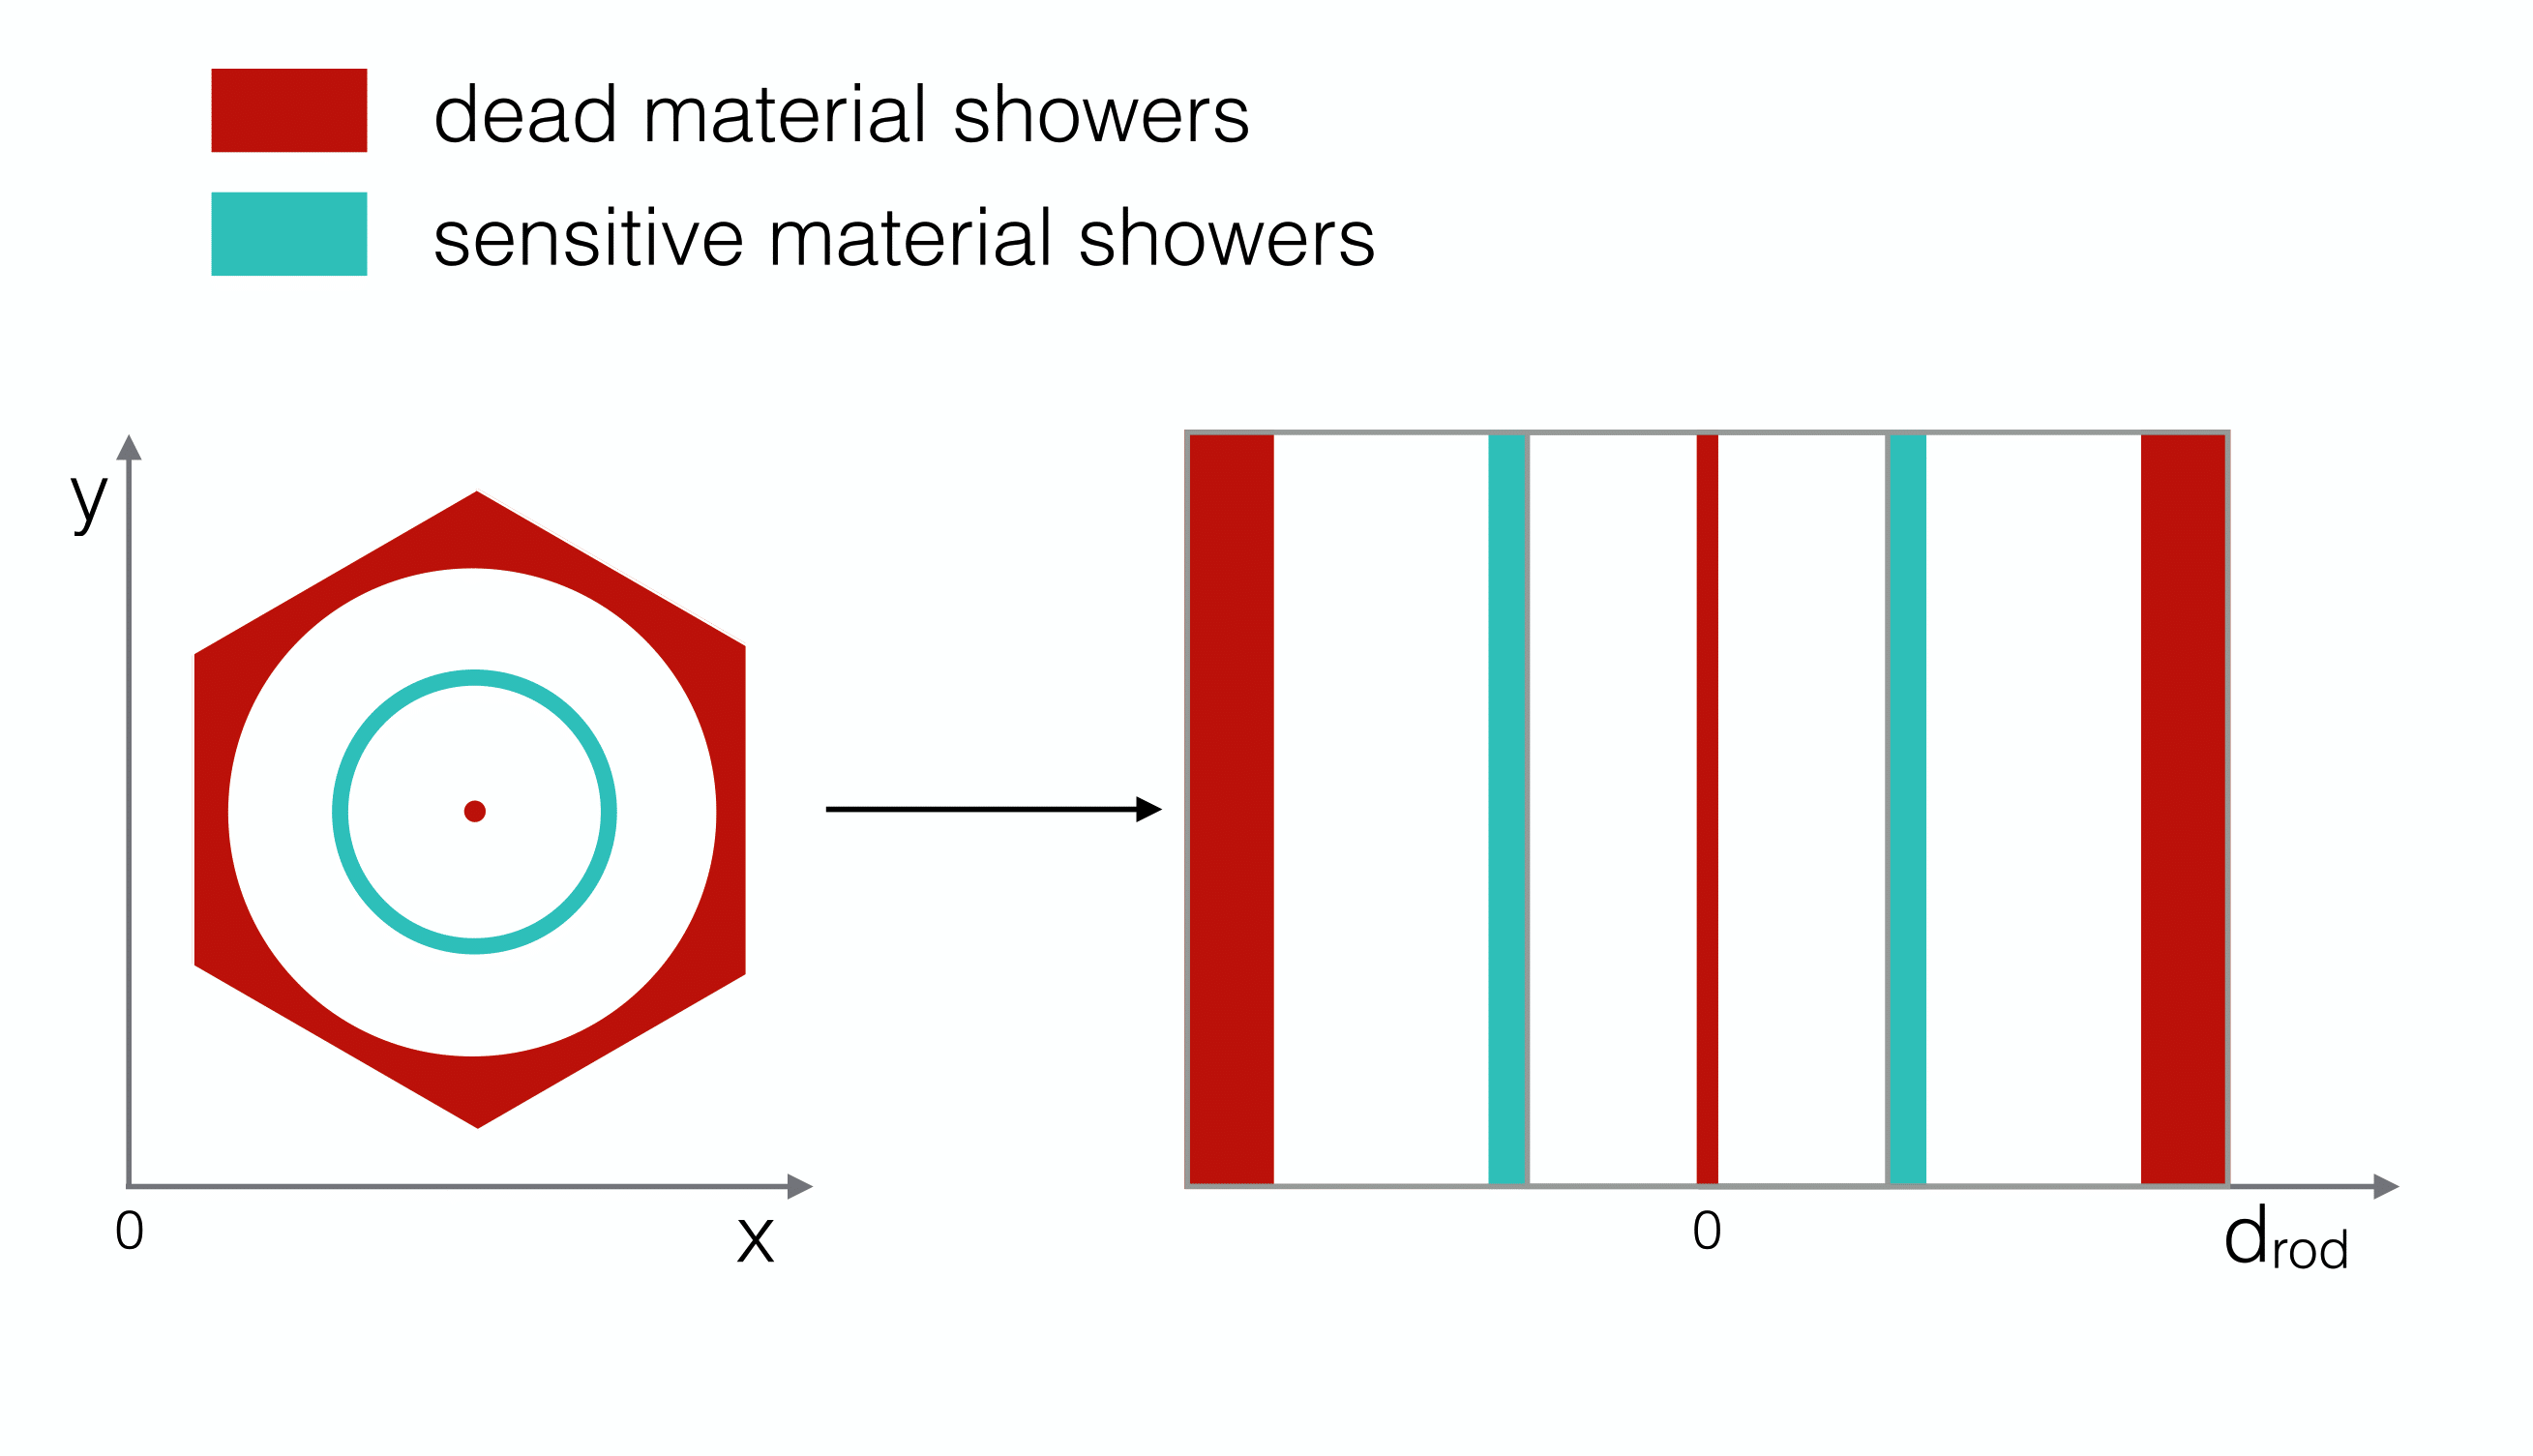
\includegraphics[width=1.0\textwidth]{MC/FirstClassifierData.png}
\caption{Schematic representation of preselected data for a first classifier in x vs y (left) and distance(right) plane. Electrons, created near the rod center and on the borders of the module have low probability to cross the sensitive material, while those created inside liquid argon gap belong to sensitive material showers.}
\label{fig:SchemePresel}}
\end{figure}

\subsubsection{Second classifier}

\begin{figure}[!tbp]
\begin{minipage}[h]{0.49\linewidth}
\center{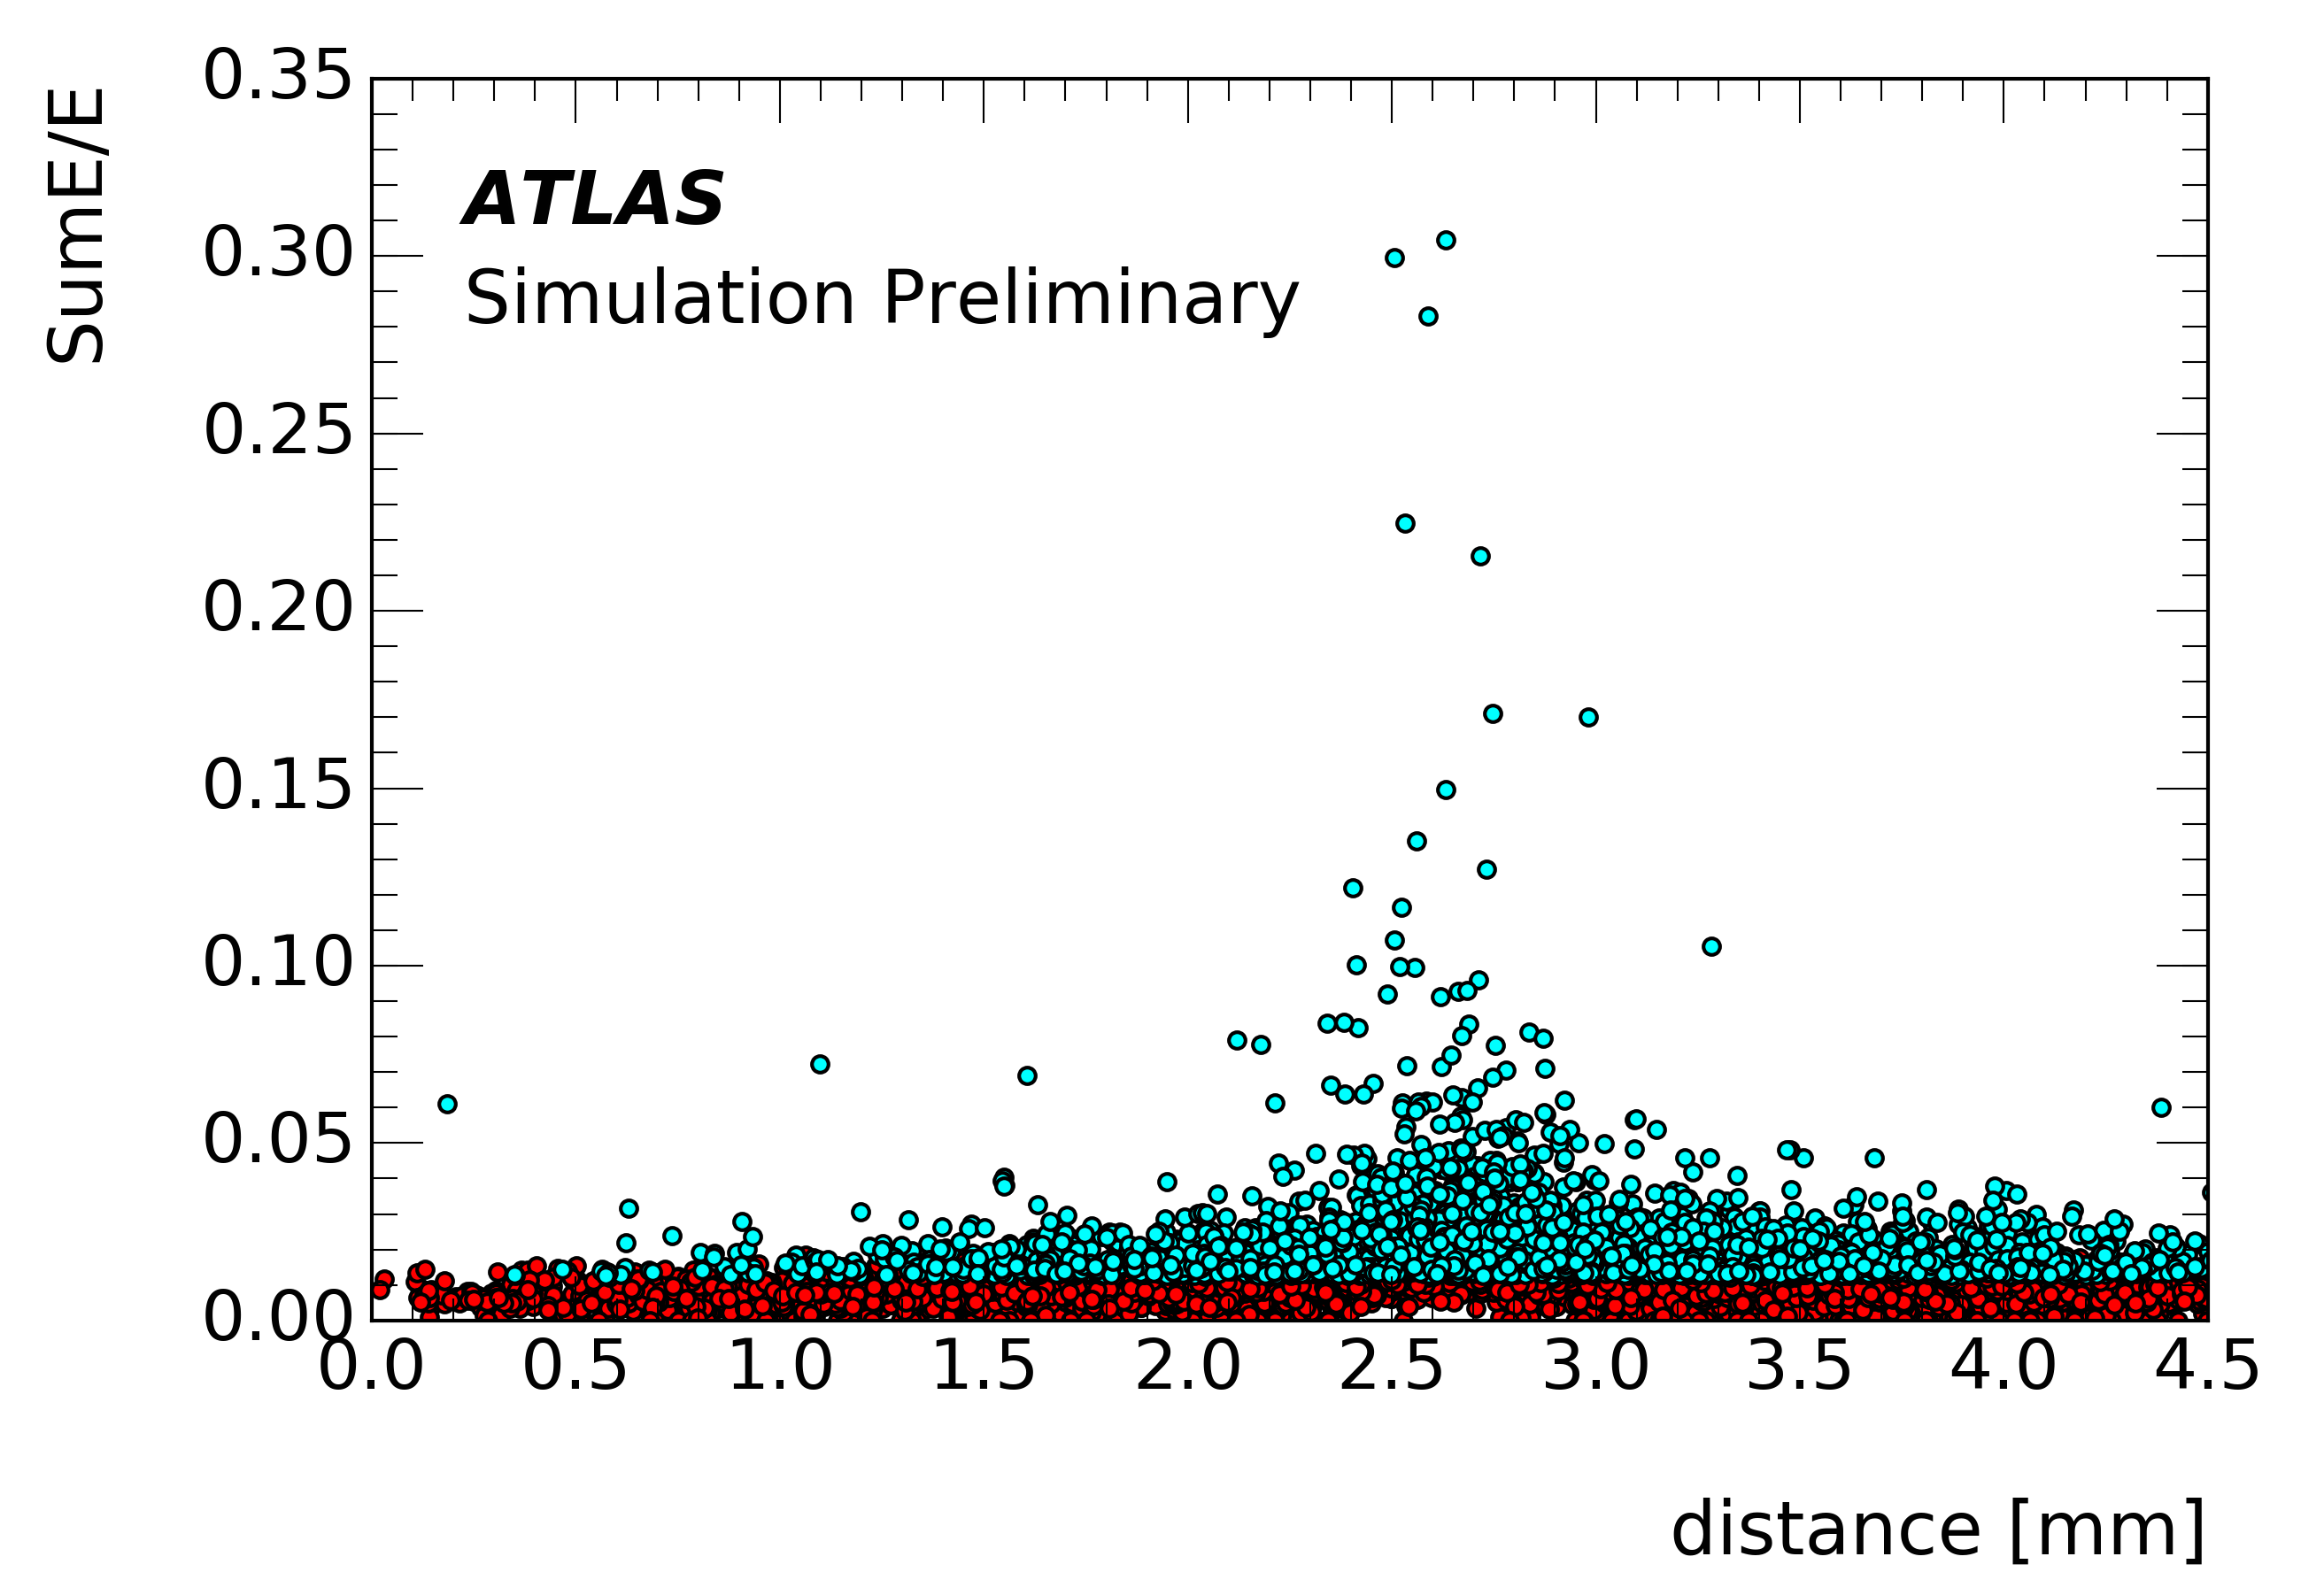
\includegraphics[width=1.\linewidth]{MC/firstClassifier.png} \\ a)}
\end{minipage}
\hfill
\begin{minipage}[h]{0.49\linewidth}
\center{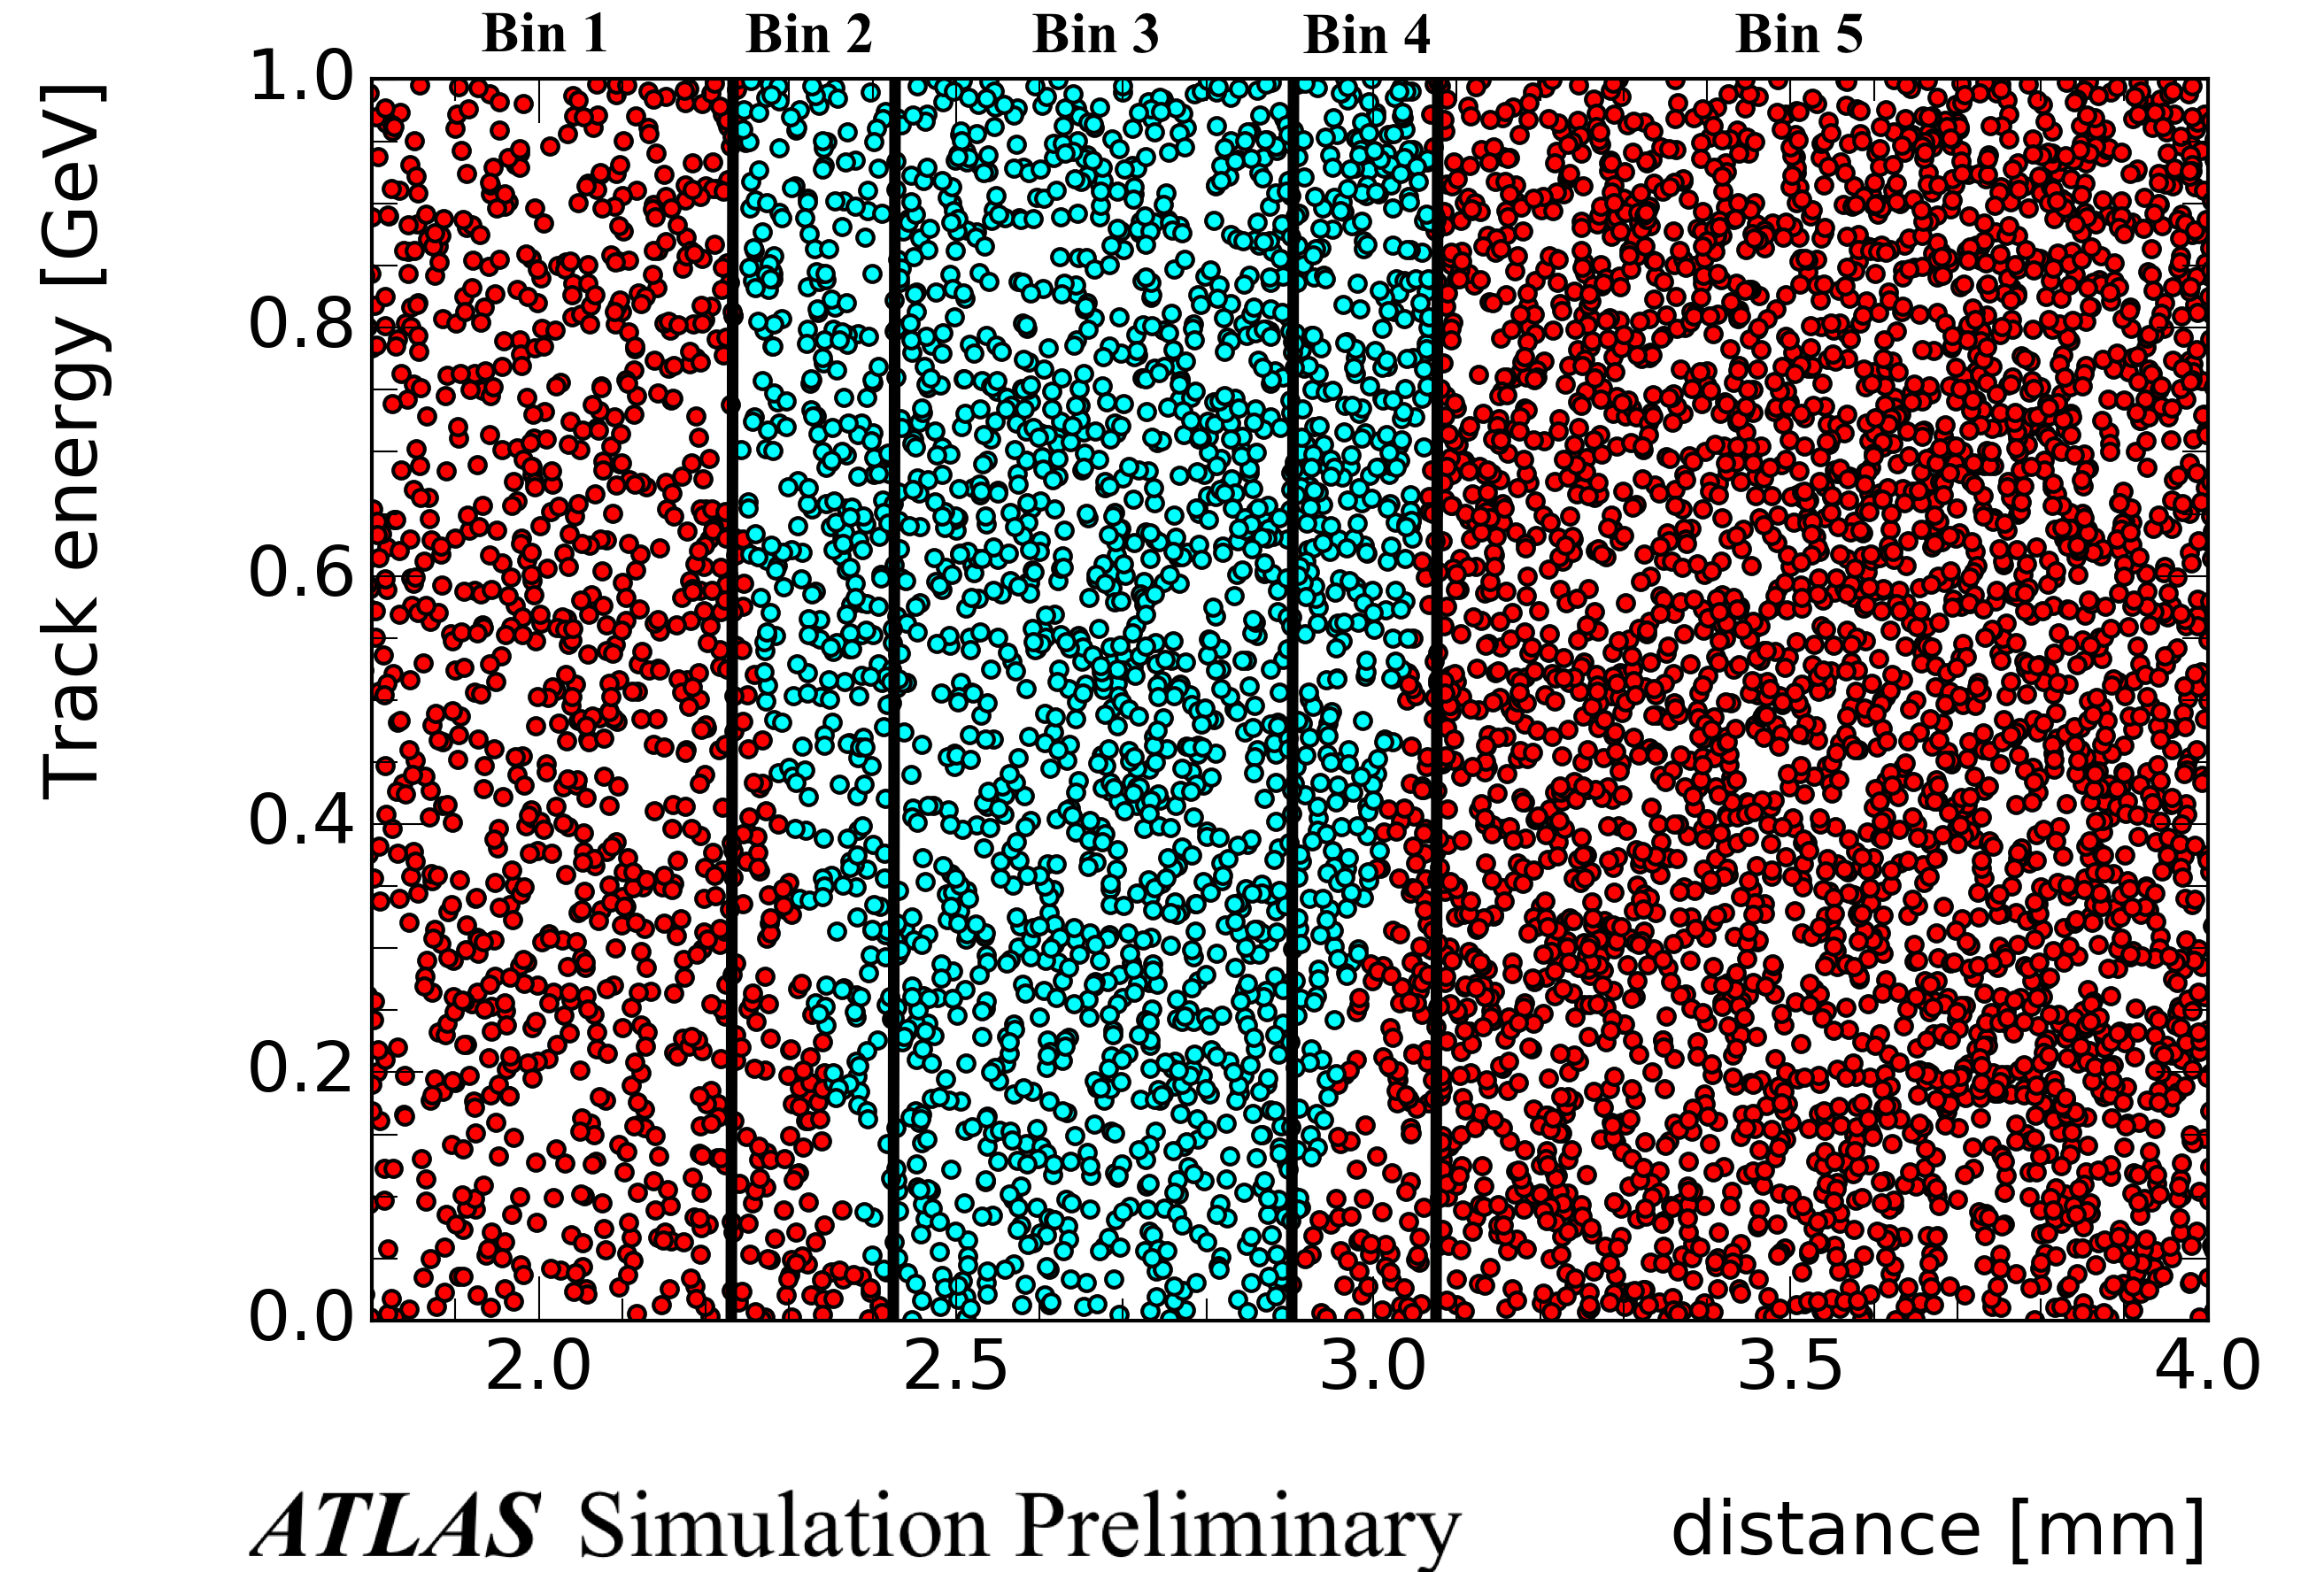
\includegraphics[width=1.\linewidth]{MC/secondClassifier.png} \\ b)}
\end{minipage}
\caption{Results of machine learning algorithm classification for a) first classifier b) second classifier. Cyan dots correspond to sensitive material showers, red to dead material showers. Black lines in Fig. b correspond to resulting bin positions}
\label{fig:Class}
\end{figure}

The second classifier uses predictions of the first classifier as an input label. It is trying to reconstuct a best dividing hyperplane between two methods using a support vector machines. It uses as an input truth parameters of the electron, e.g. energy of the initial electron and its distance to a closest rod center. Different kernels have been tested and the best predictions have been obtained using RBF kernel (Eq. \ref{eq:RBF}).  Assuming, that $\eta^{momentum} \approx \eta^{position}$ classification is performed in each $\eta^{distance}$ bin used in a library. Example of the classifier output is shown in a Fig. \ref{fig:Class} b). As it is expected from the model, that the gap position is getting wider with higher energies of the electron.  Variation of the obtained parameters have been found small, so the mean of the parameters has been used.  

\subsection{Interpretation of results}

Because a full new regeneration of libraries and the validation of reconstructed variables is a time-consuming procedure, the toy Monte-Carlo method has been developed for a cross-check of classifiers and its interpretation. It uses pseudorapidity $\eta^{position}$, energy of electron and distance to a closest rod center from data as a reference for a random generator. This simulation allows to compare shower energies and shower energies divided by  the energy of the initial electron (SumE/E) distributions with distributions coming from full simulation, that are considered as a reference.

Several interpretations of the bin positions have been tested and the best one is shown in Fig. ~\ref{fig:Class} b) with black lines. It was decided to make 3 bins in liquid argon position instead of having only one. One bin contains, according to a classifier, just sensitive material showers events, while the other 2 there is a mixture of dead and sensitive material showers. The obtained positions of the liquid argon bins are wider, than the nominal ones for both FCAL1 and FCAL2, as expected from the model.

Comparison of SumE/E distributions using toy MC on old libraries (Fig. ~\ref{fig:Interpret} a) and the libraries with the new binning (Fig. ~\ref{fig:Interpret} b) has shown, that we could expect a better performance on reconstructed values.

\begin{figure}[!tbp]
\begin{minipage}[h]{0.49\linewidth}
\center{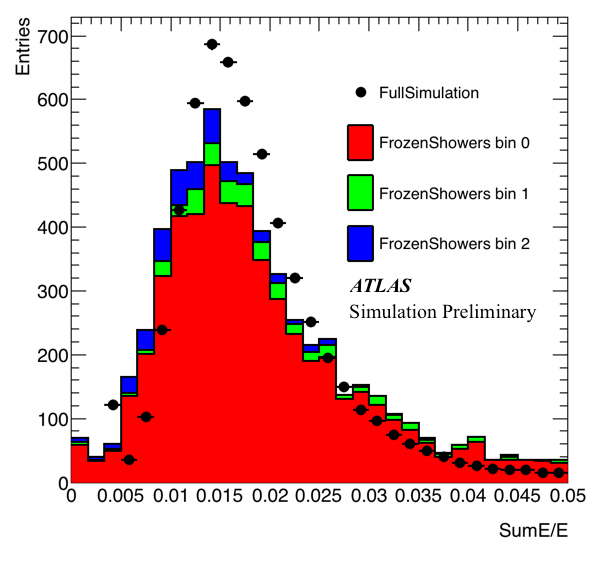
\includegraphics[width=1.\linewidth]{MC/oldSumE.png} \\ a)}
\end{minipage}
\hfill
\begin{minipage}[h]{0.49\linewidth}
\center{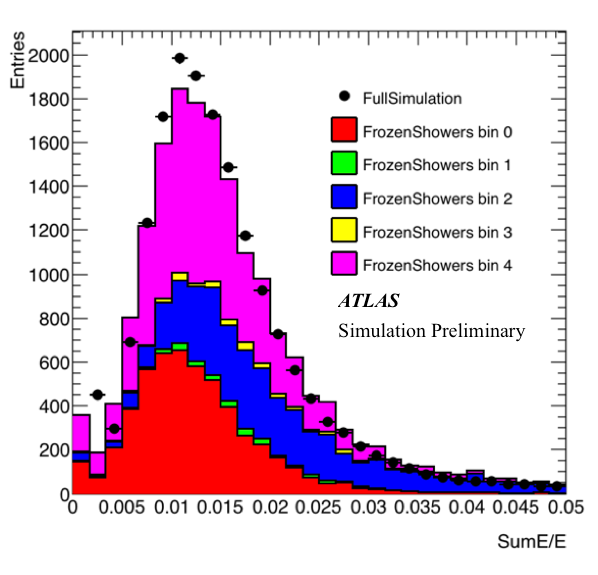
\includegraphics[width=1.\linewidth]{MC/newSumE.png} \\ b)}
\end{minipage}
\caption{Comparison of the distributions of shower energy divided by  the energy of the initial electron between full simulation and toy MC using libraries for liquid argon gap bins and 2 closest to them bins for a) old "tuned" libraries with 1 liquid argon gap bin  b) new libraries using 3 liquid argon gap bins. There are still remaining differences between full simulation and toy MC, but the new machine learning binning gives a better agreement with full simulation.}
\label{fig:Interpret}
\end{figure}


\subsection{Reconstructed electron energy}

Since the resolution of the single electrons can have a significant difference, the energies of reconstructed electrons are validated before the mass validation of the different groups. Measurement of the shift in the mean energy between full and fast simulation allows to correct the scale for frozen showers.

Validation is performed for the following electron energies: 100 GeV, 200 GeV, 500 GeV and 1000 GeV and within the $\eta$ directions that are corresponding to the 12 $\eta$ bins of the library. The resolution is calculated as RMS of all reconstructed energies for the certain energy and $\eta$. The results of the electron resolution validation for the new machine learning based binning and old "tuned" libraries is shown in Fig. \ref{fig:Reso}. The new methods gives a better of comparable resolution agreement than an old libraries. However, there are 2 bins, there new method resolution is significantly worse, than old one (3.5 and 4.3). This means, that this method still needs to be improved. The possible ways of its improvement are discussed in Sec. \ref{sec:FSImpr}.

In a meanwhile it was decided to use a combination of the new and old libraries. The mean shift is corrected as described in Sec. \ref{sec:LibTuning} and showed in Fig. \ref{fig:Mean}. The remaining differences between full and fast simulation are considered negligible.


\begin{figure}[!tbp]
\begin{minipage}[h]{0.32\linewidth}
\center{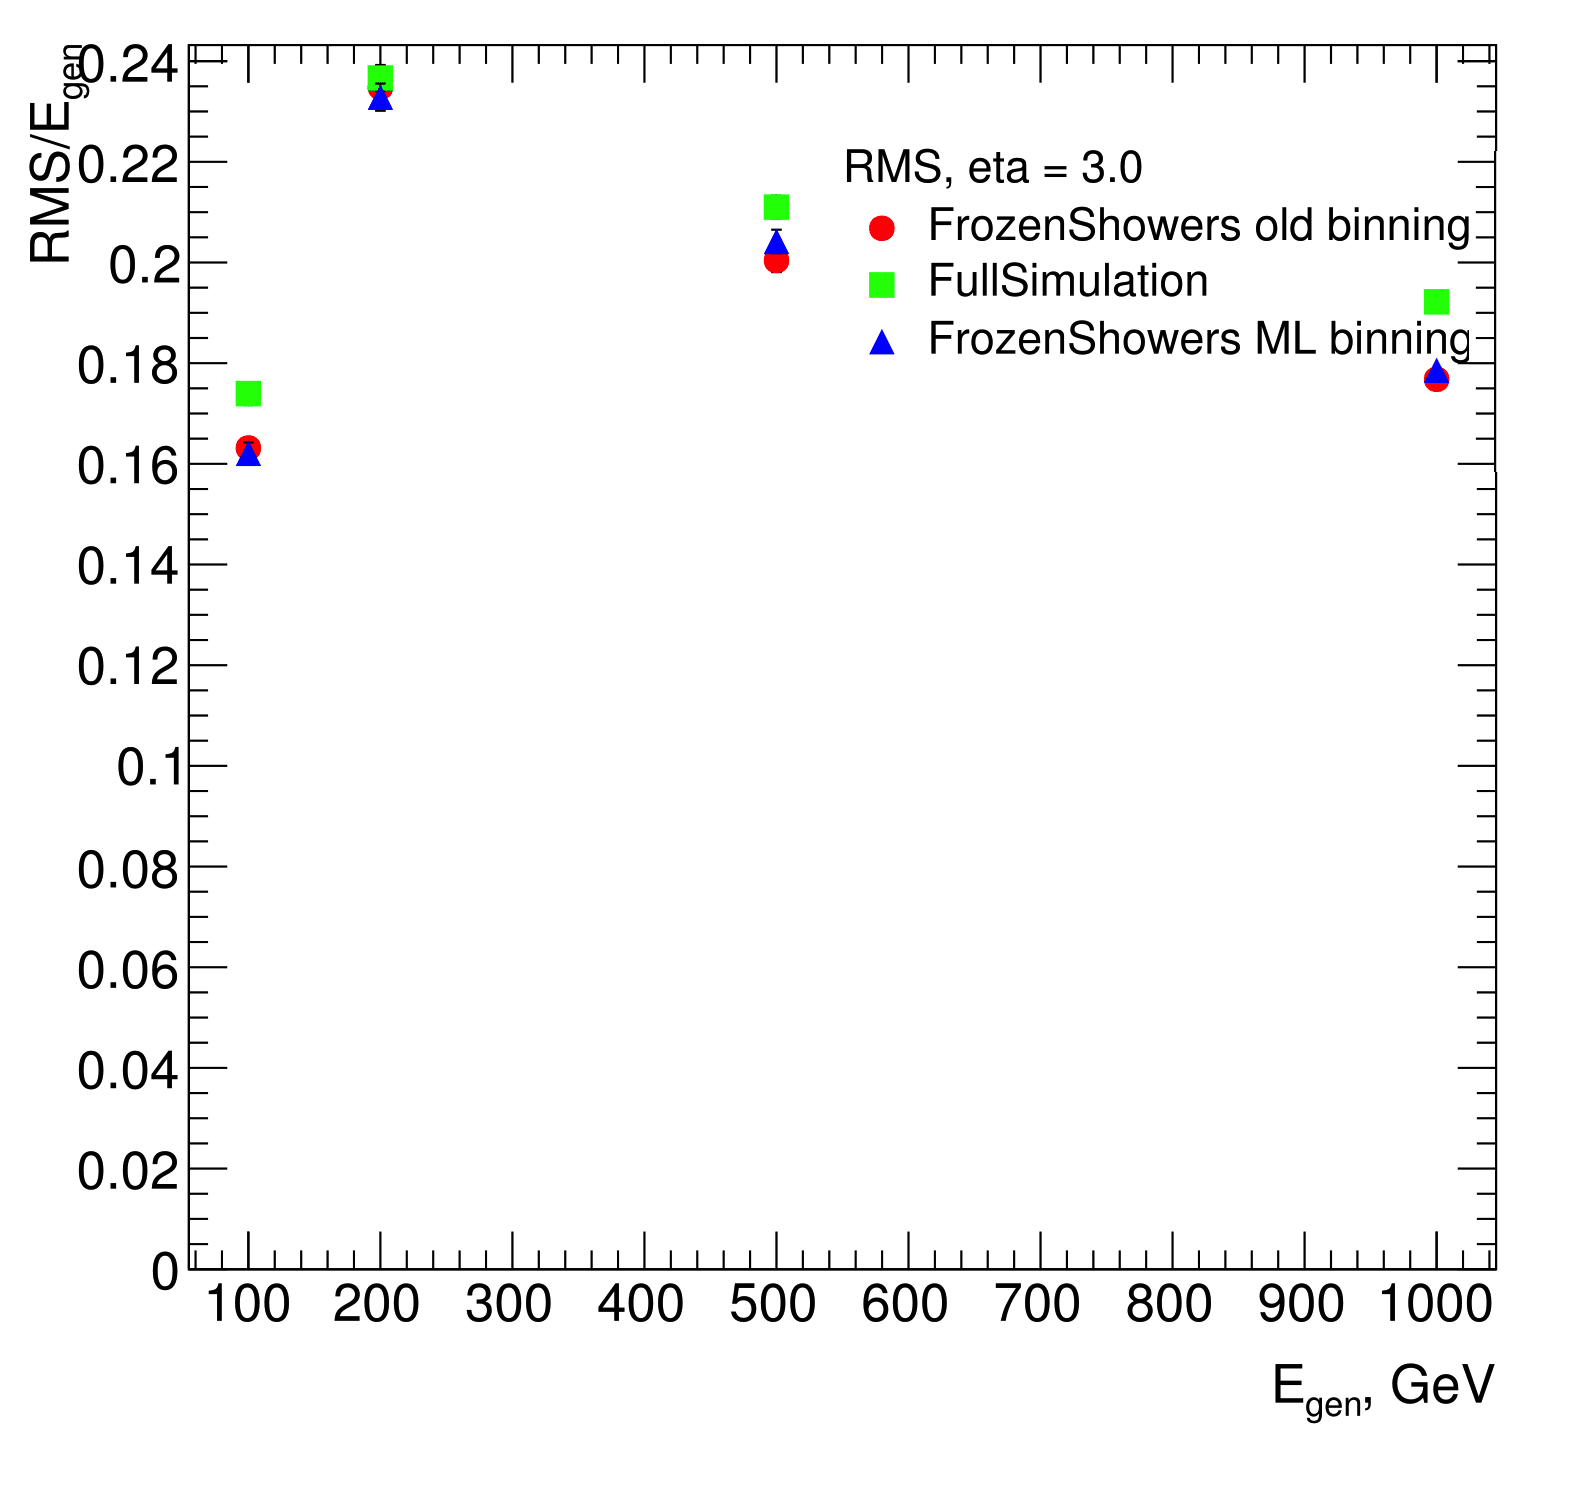
\includegraphics[width=1.\linewidth]{MC/RMS/RMS-12.png} }
\end{minipage}
\hfill
\begin{minipage}[h]{0.32\linewidth}
\center{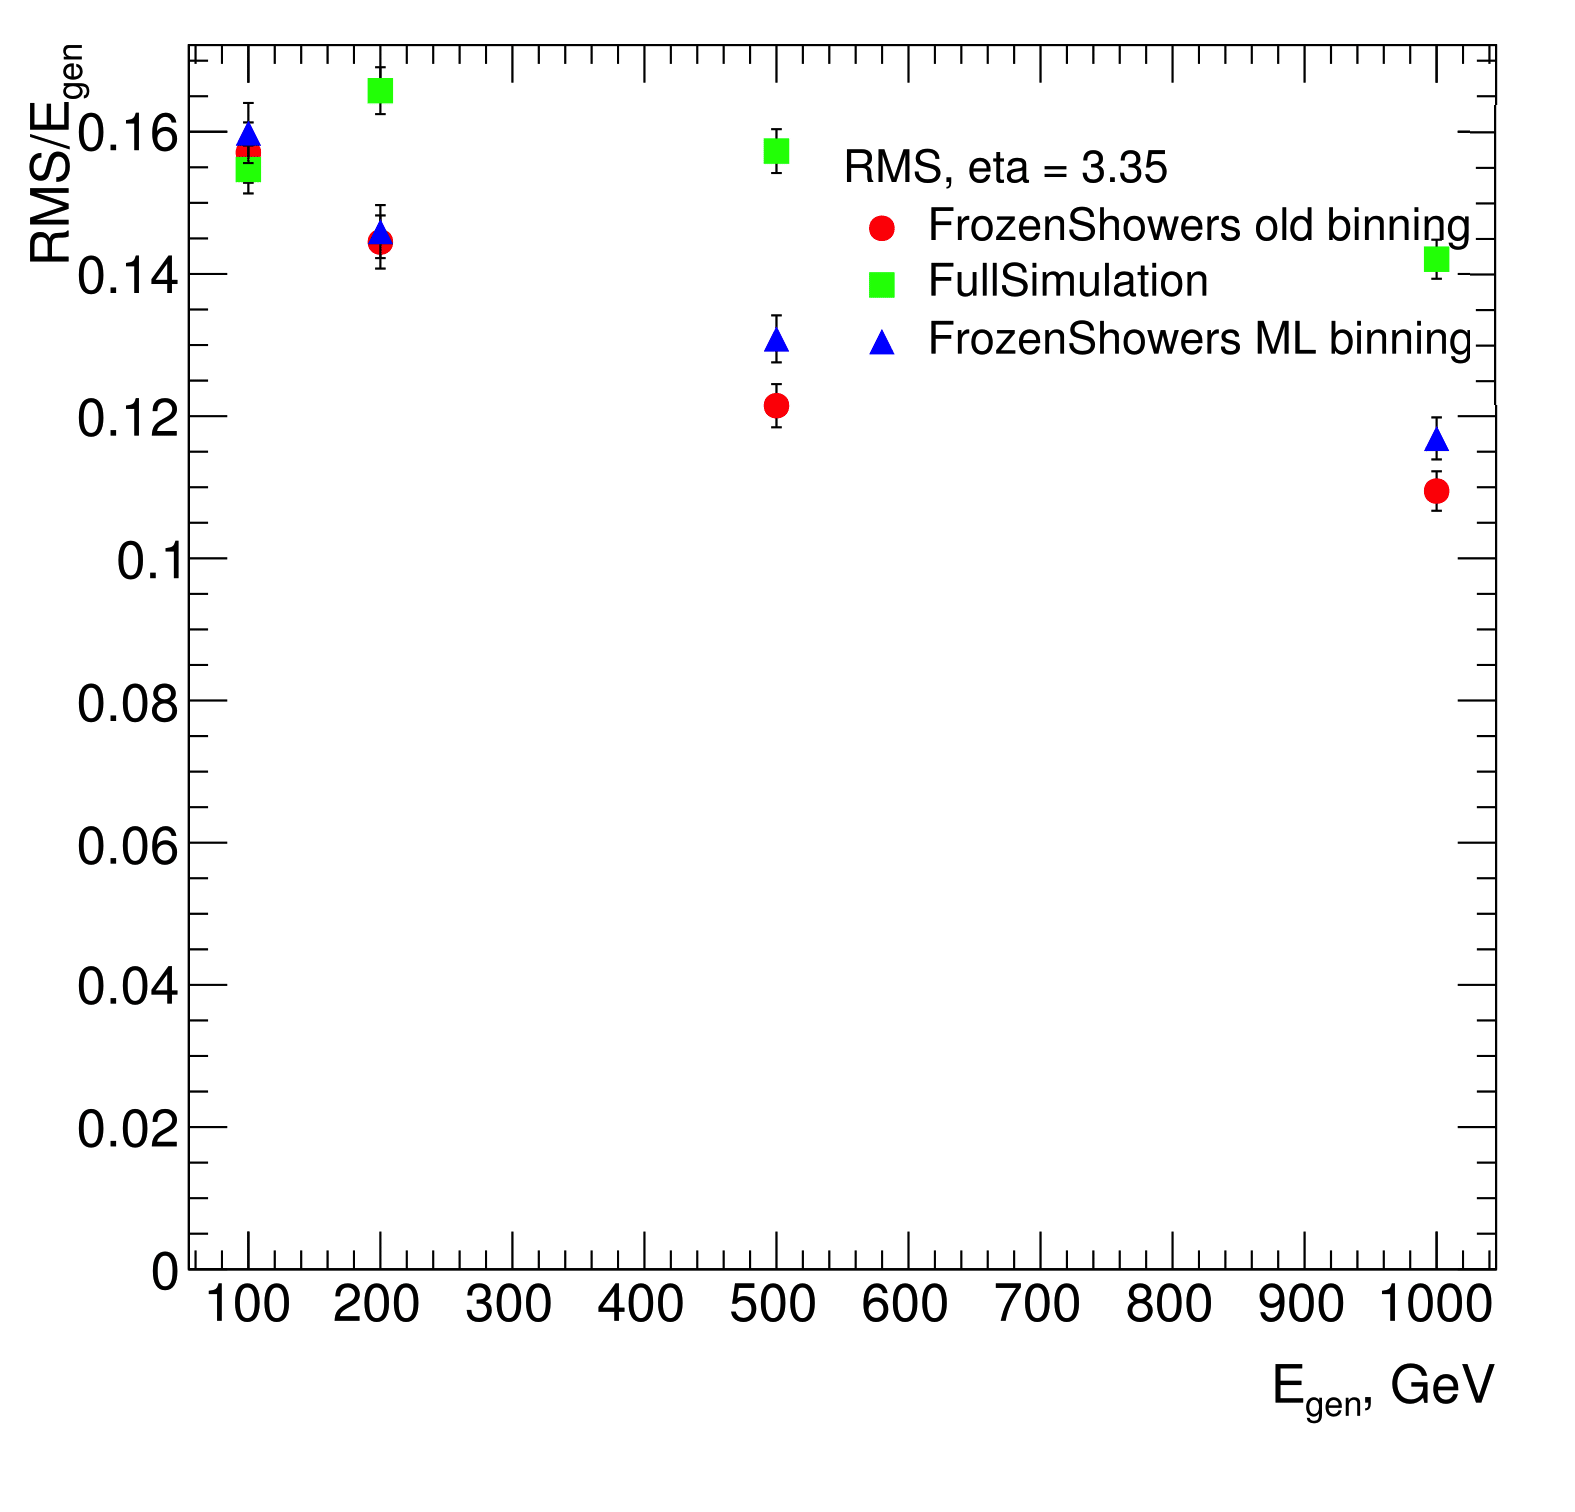
\includegraphics[width=1.\linewidth]{MC/RMS/RMS-11.png} }
\end{minipage}
\hfill
\begin{minipage}[h]{0.32\linewidth}
\center{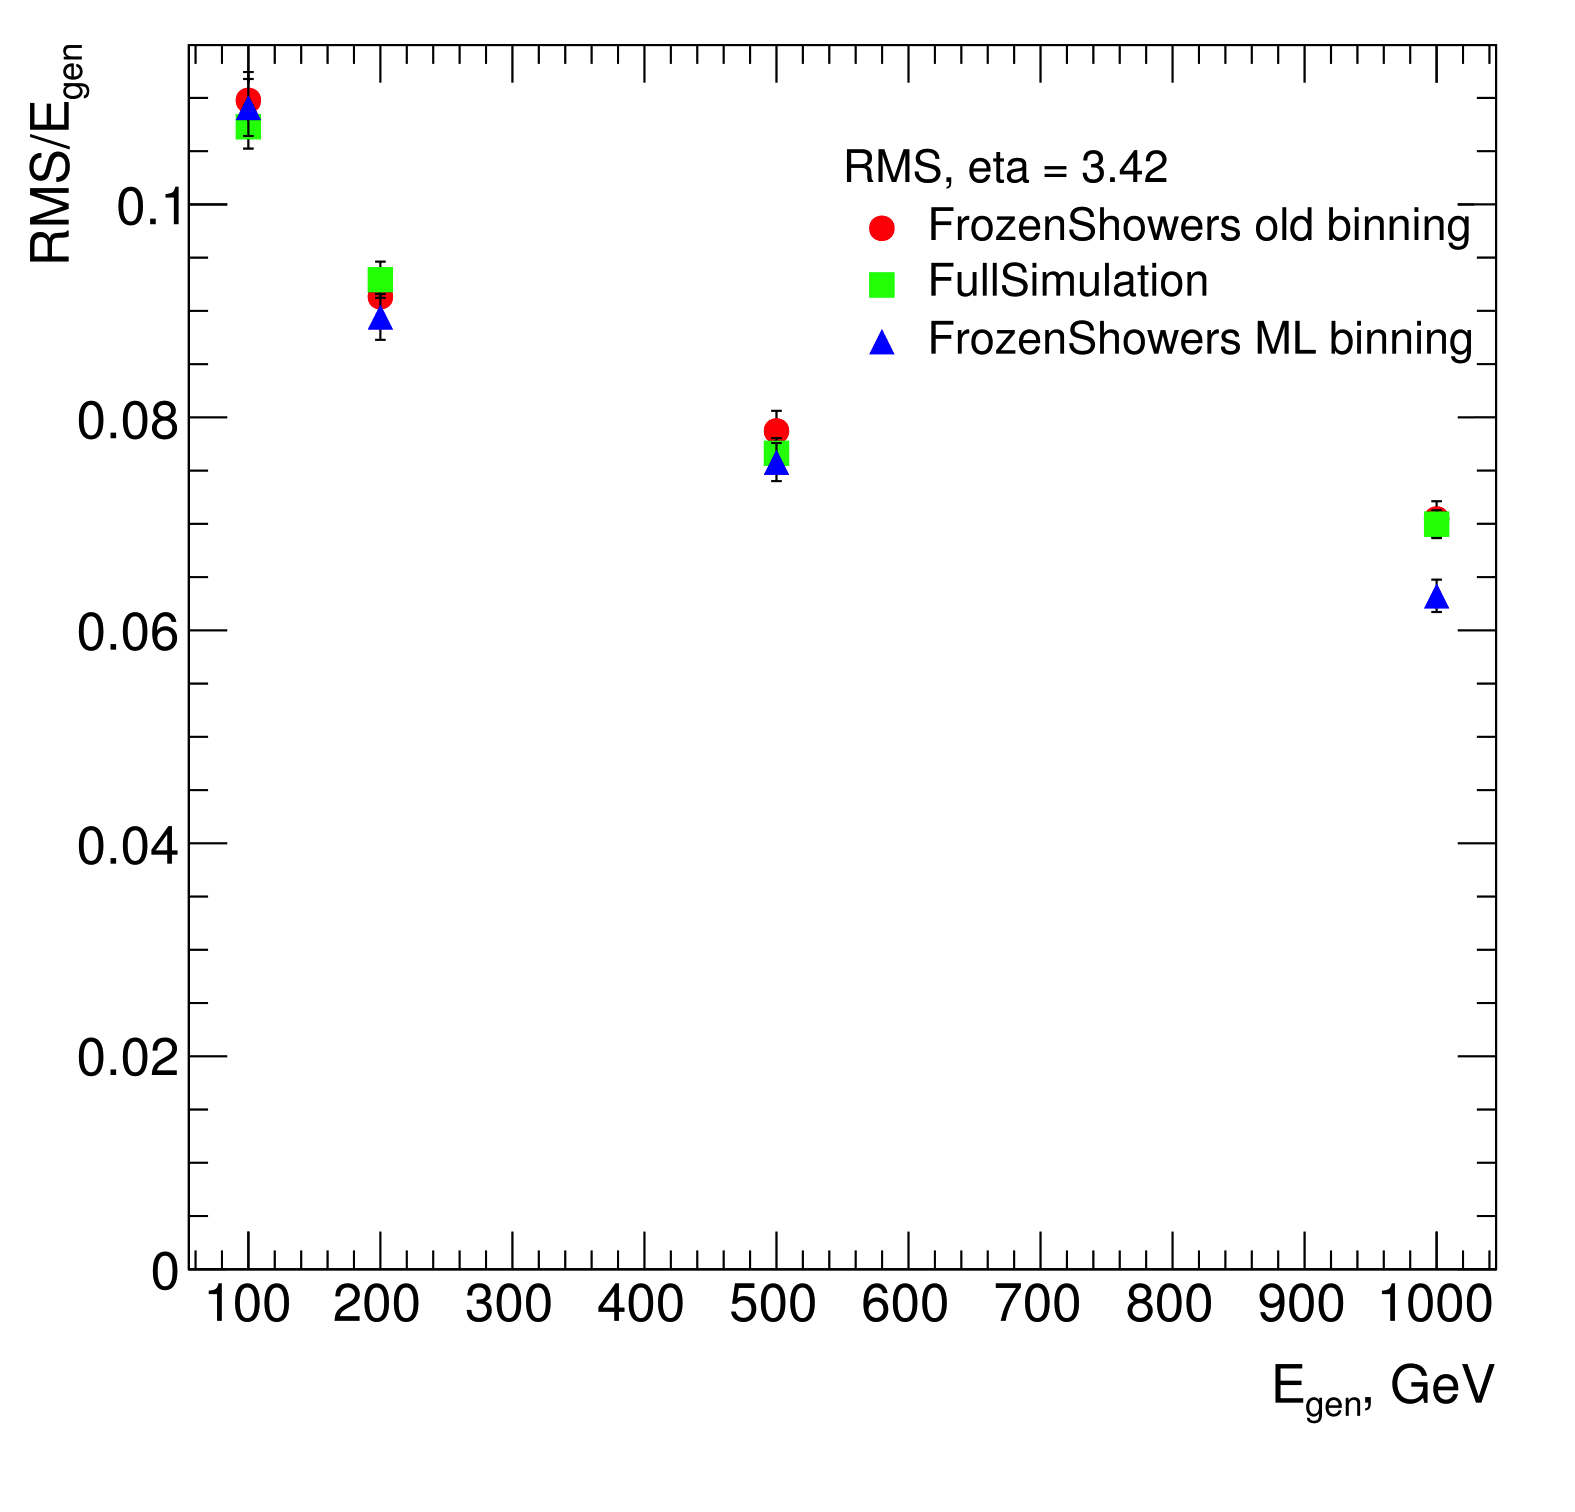
\includegraphics[width=1.\linewidth]{MC/RMS/RMS-10.png}  }
\end{minipage}
\vfill
\begin{minipage}[h]{0.32\linewidth}
\center{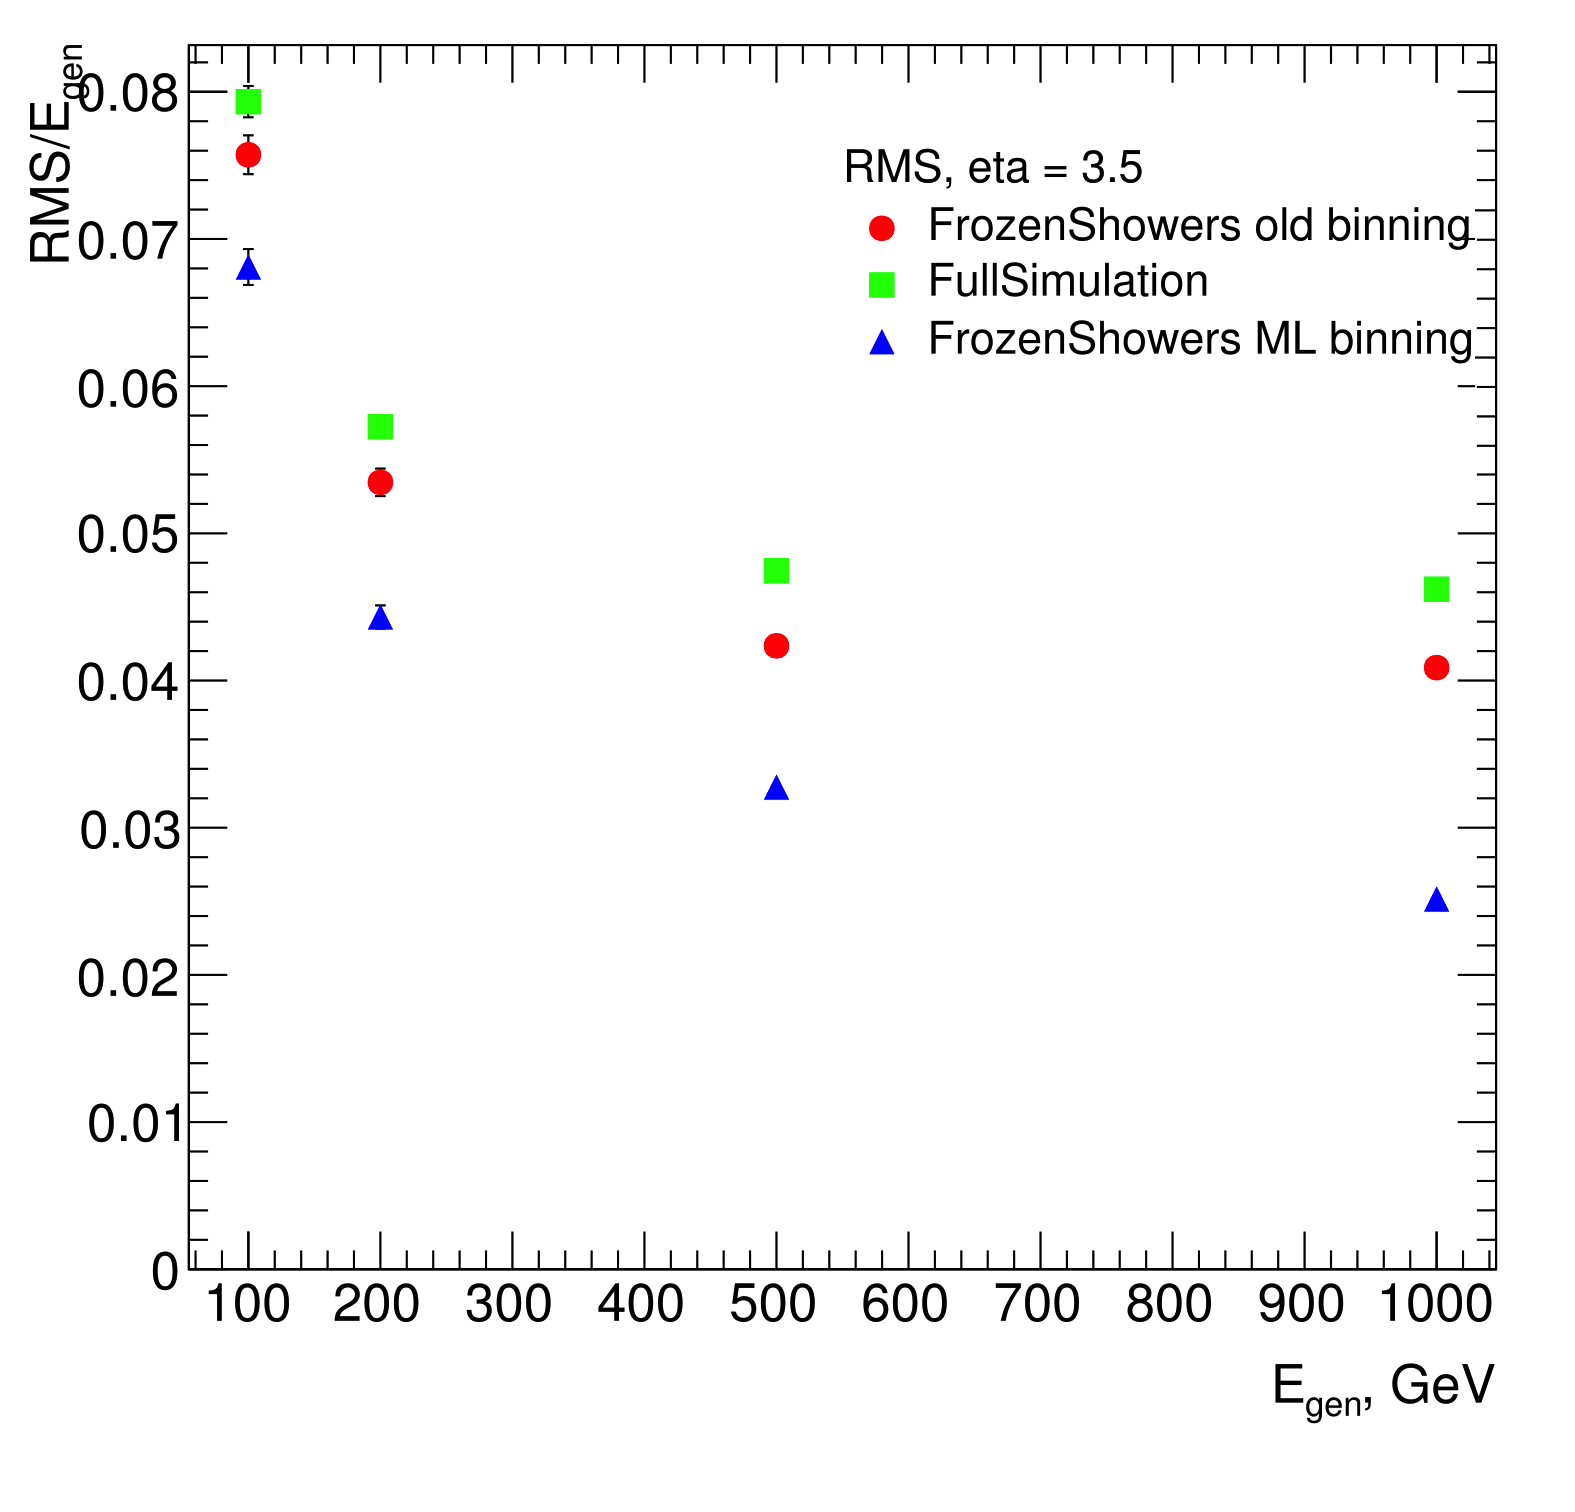
\includegraphics[width=1.\linewidth]{MC/RMS/RMS-09.png}  }
\end{minipage}
\hfill
\begin{minipage}[h]{0.32\linewidth}
\center{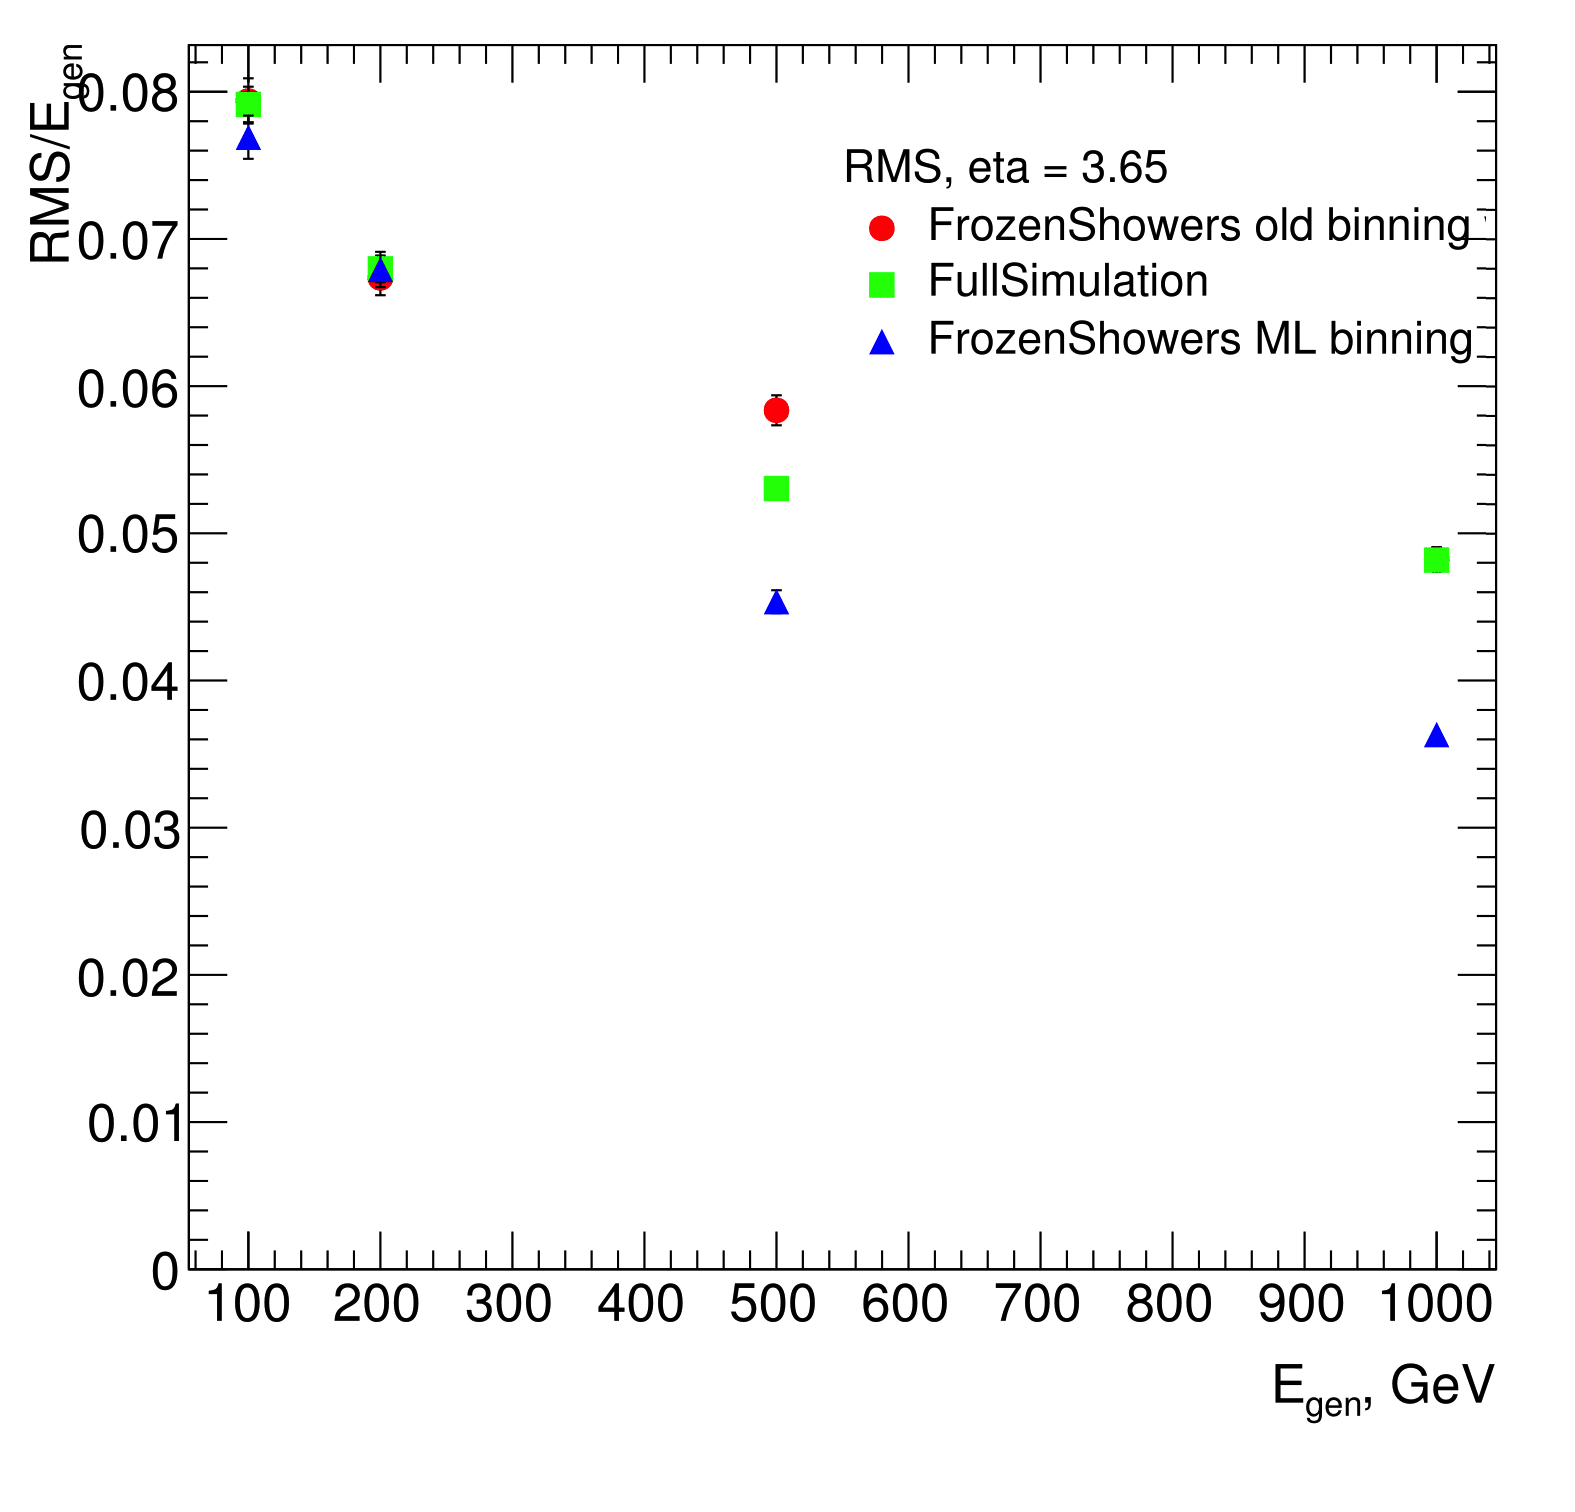
\includegraphics[width=1.\linewidth]{MC/RMS/RMS-08.png} }
\end{minipage}
\hfill
\begin{minipage}[h]{0.32\linewidth}
\center{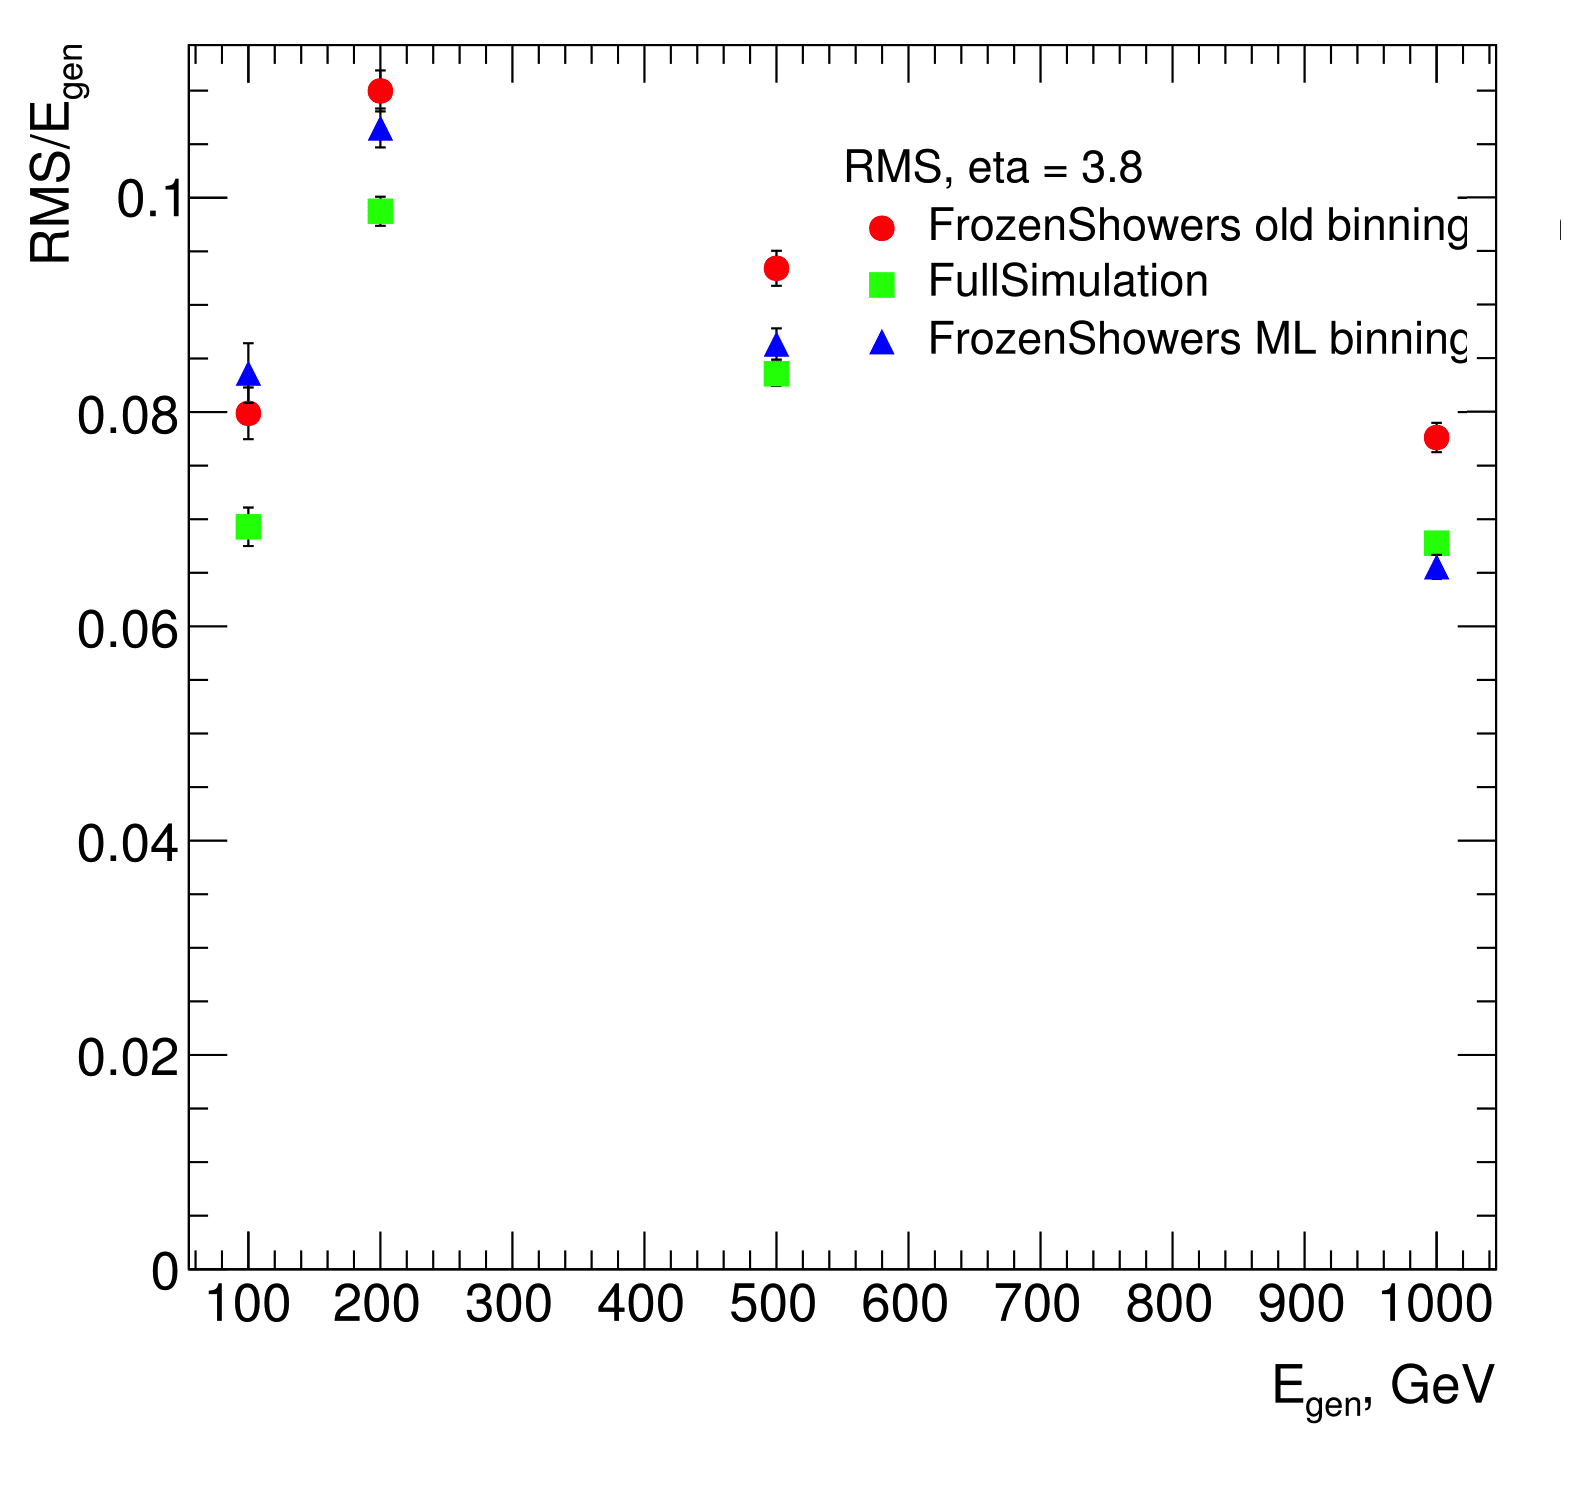
\includegraphics[width=1.\linewidth]{MC/RMS/RMS-07.png}  }
\end{minipage}
\vfill
\begin{minipage}[h]{0.32\linewidth}
\center{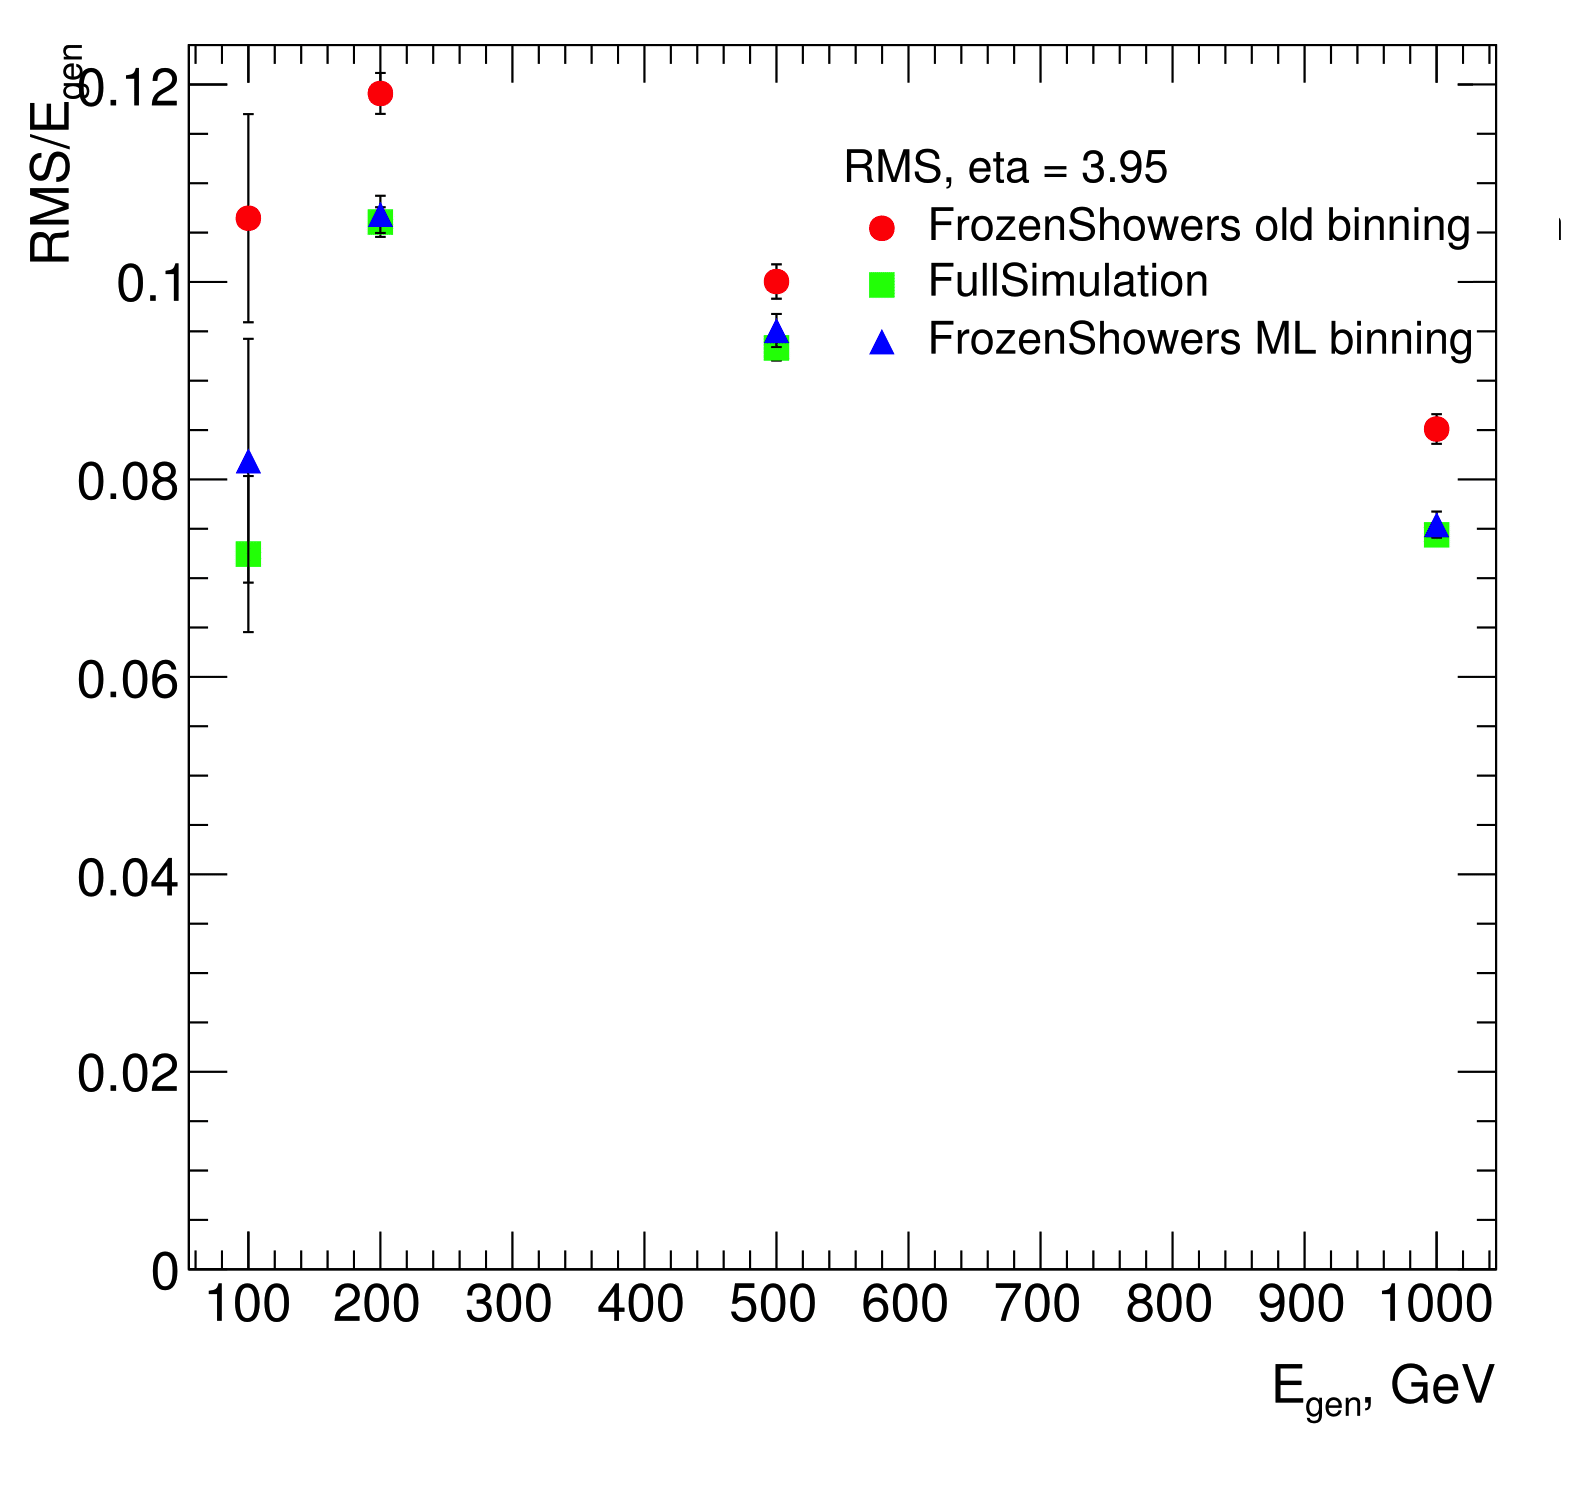
\includegraphics[width=1.\linewidth]{MC/RMS/RMS-06.png}  }
\end{minipage}
\hfill
\begin{minipage}[h]{0.32\linewidth}
\center{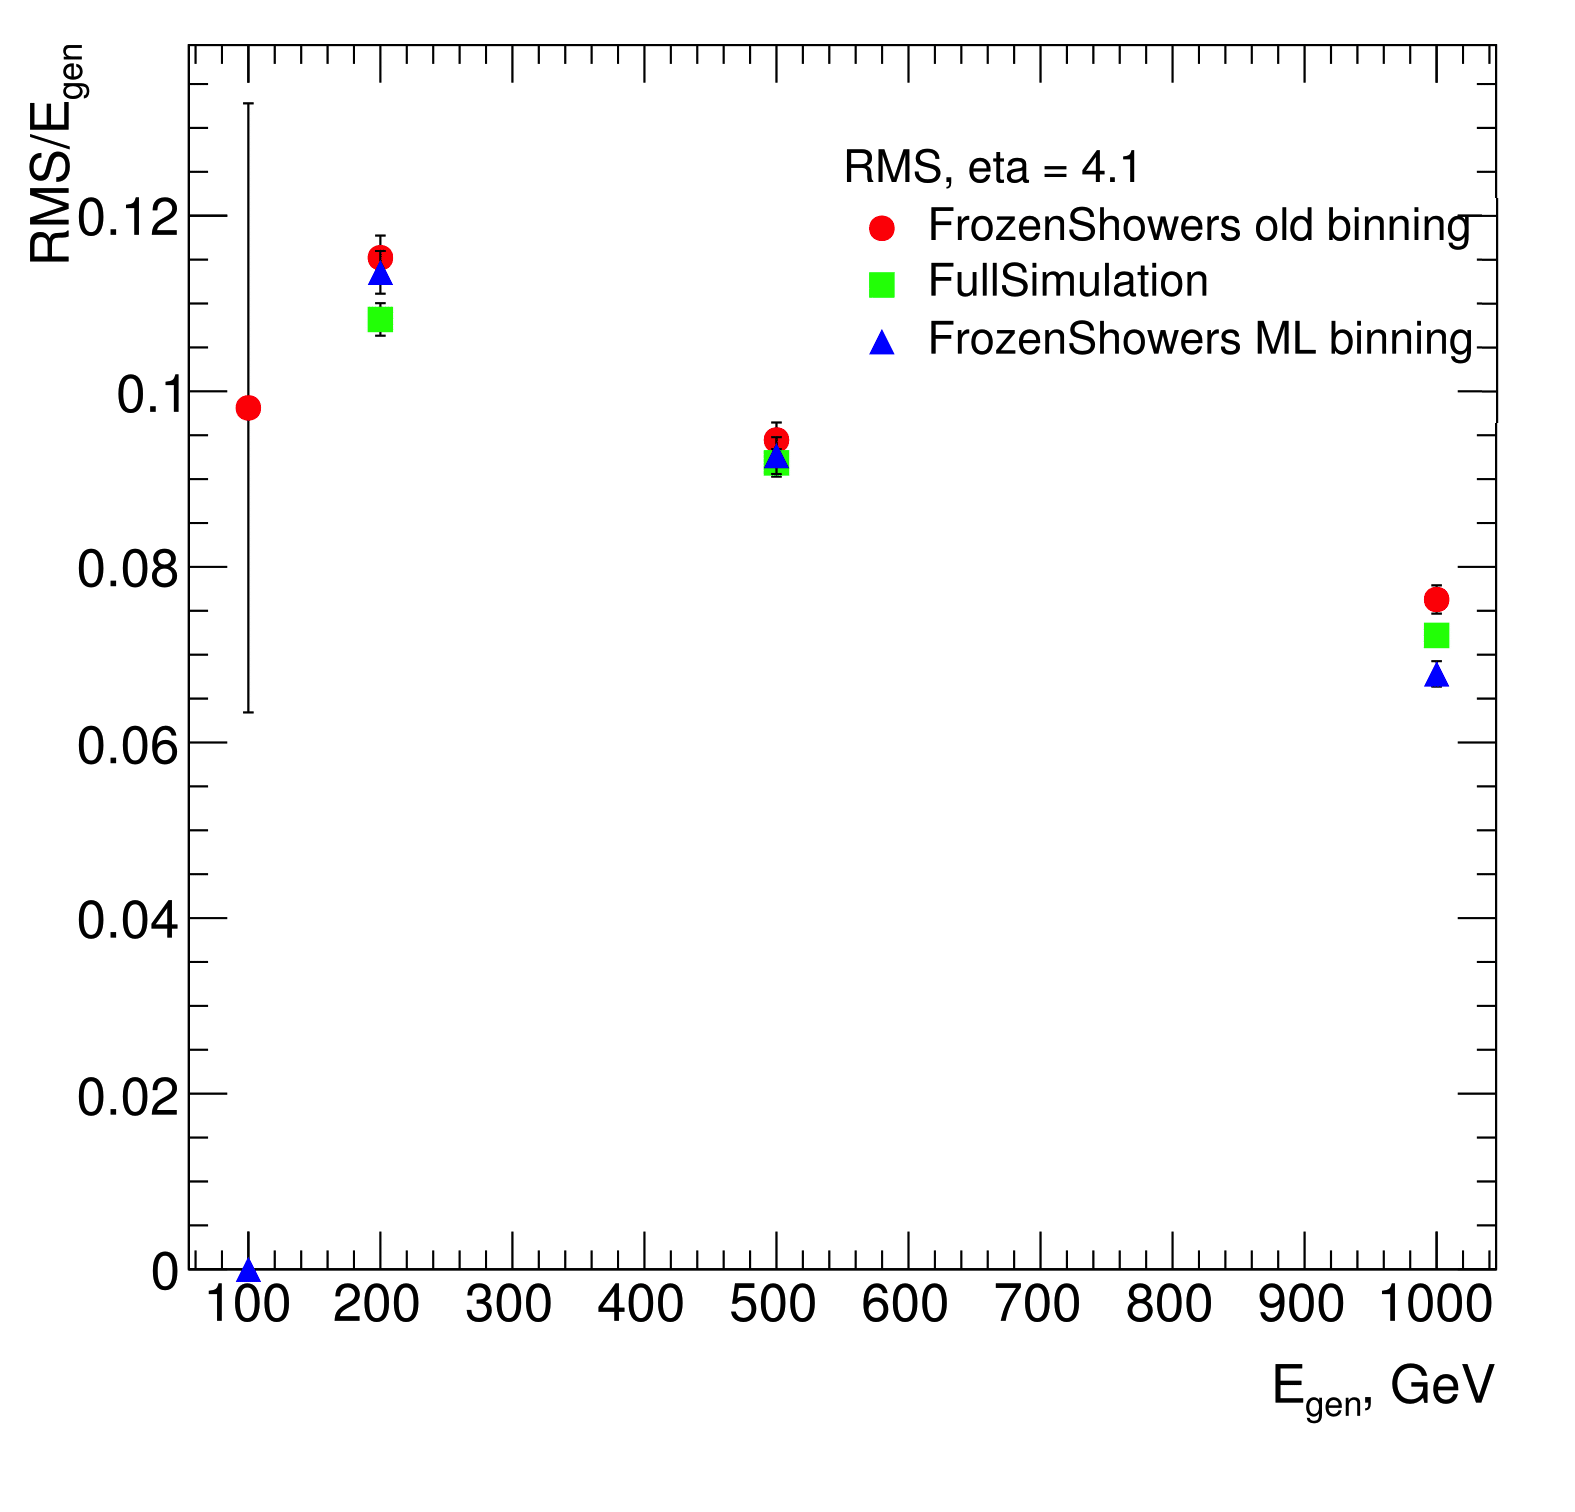
\includegraphics[width=1.\linewidth]{MC/RMS/RMS-05.png}  }
\end{minipage}
\hfill
\begin{minipage}[h]{0.32\linewidth}
\center{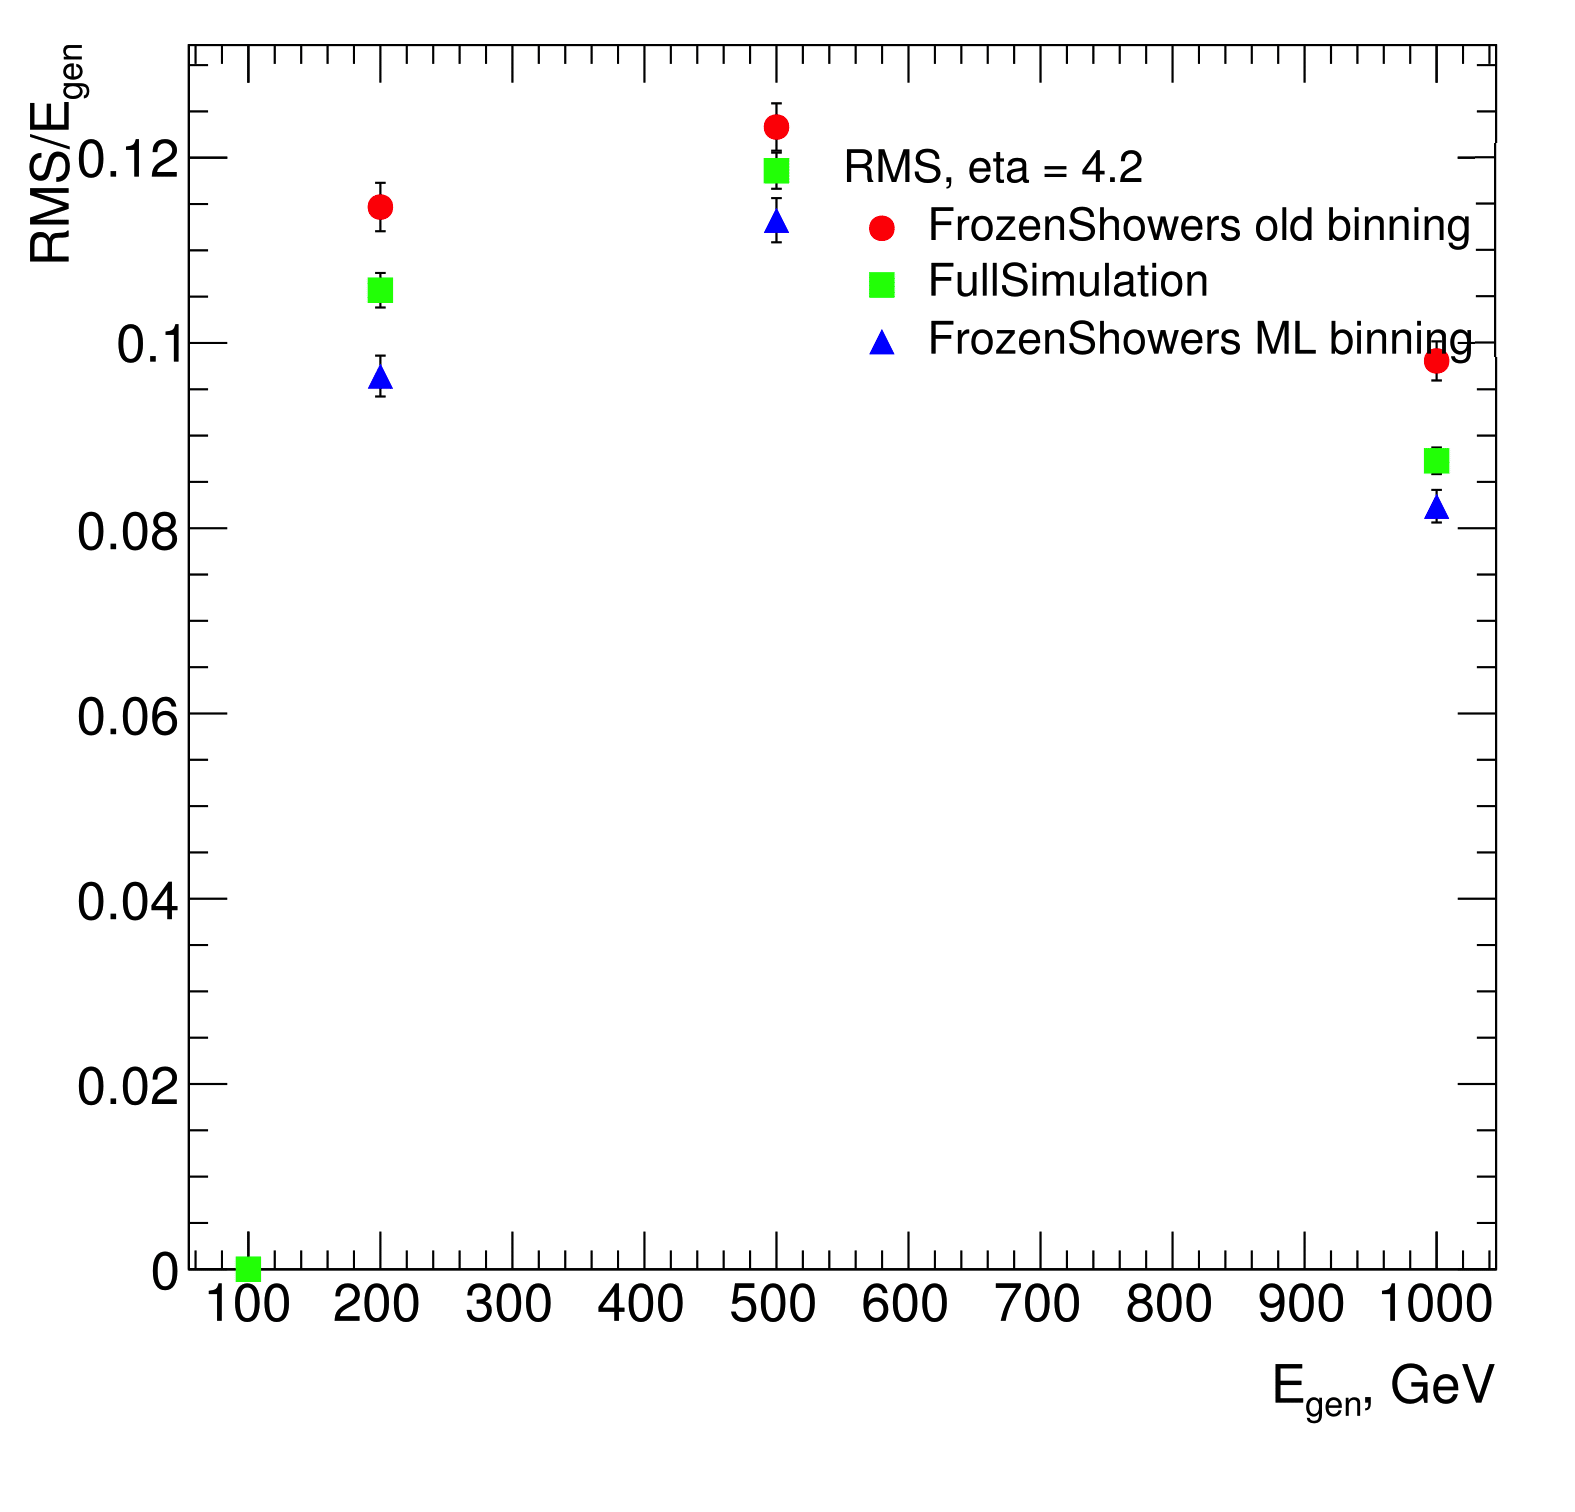
\includegraphics[width=1.\linewidth]{MC/RMS/RMS-04.png}  }
\end{minipage}
\vfill
\begin{minipage}[h]{0.32\linewidth}
\center{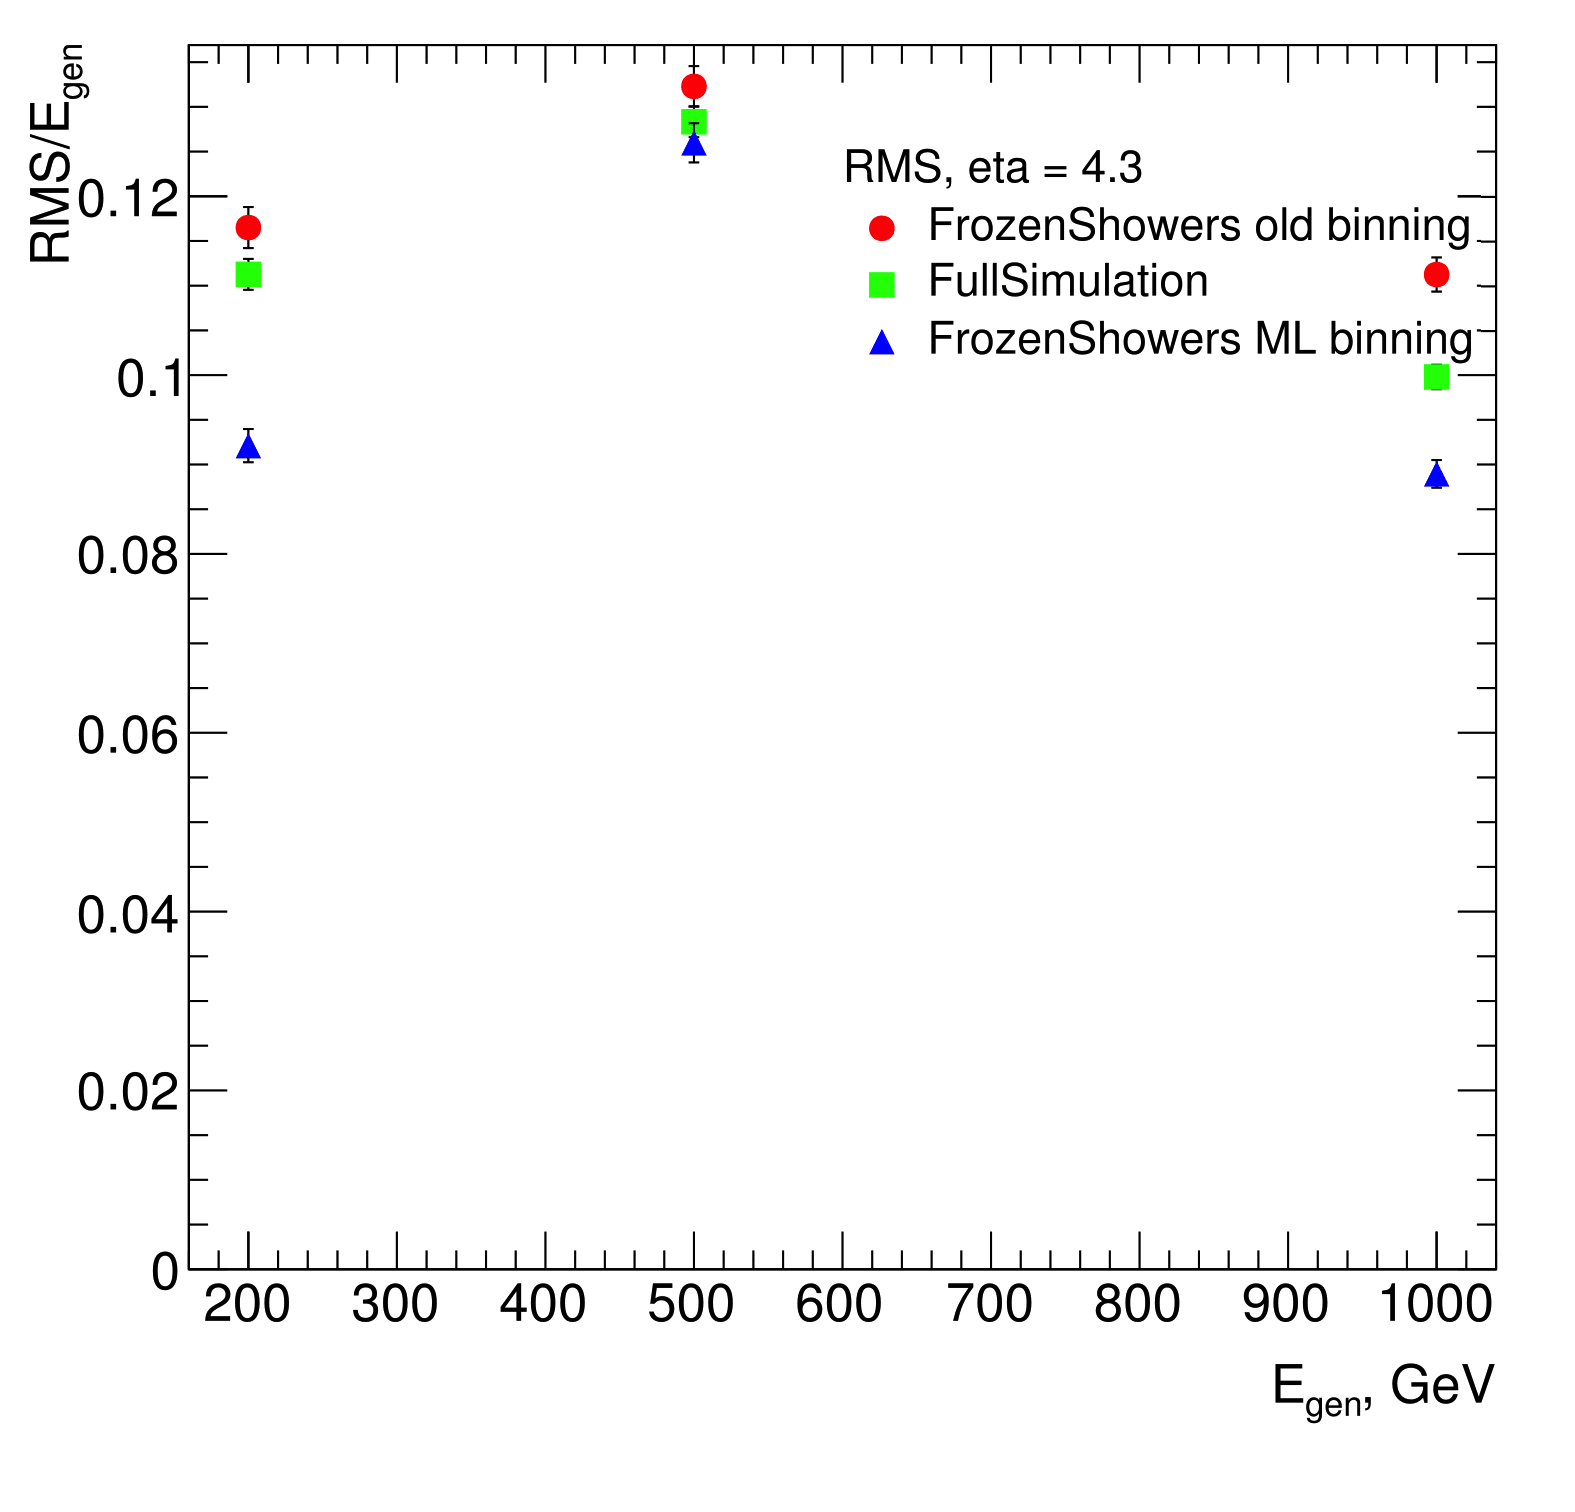
\includegraphics[width=1.\linewidth]{MC/RMS/RMS-03.png}  }
\end{minipage}
\hfill
\begin{minipage}[h]{0.32\linewidth}
\center{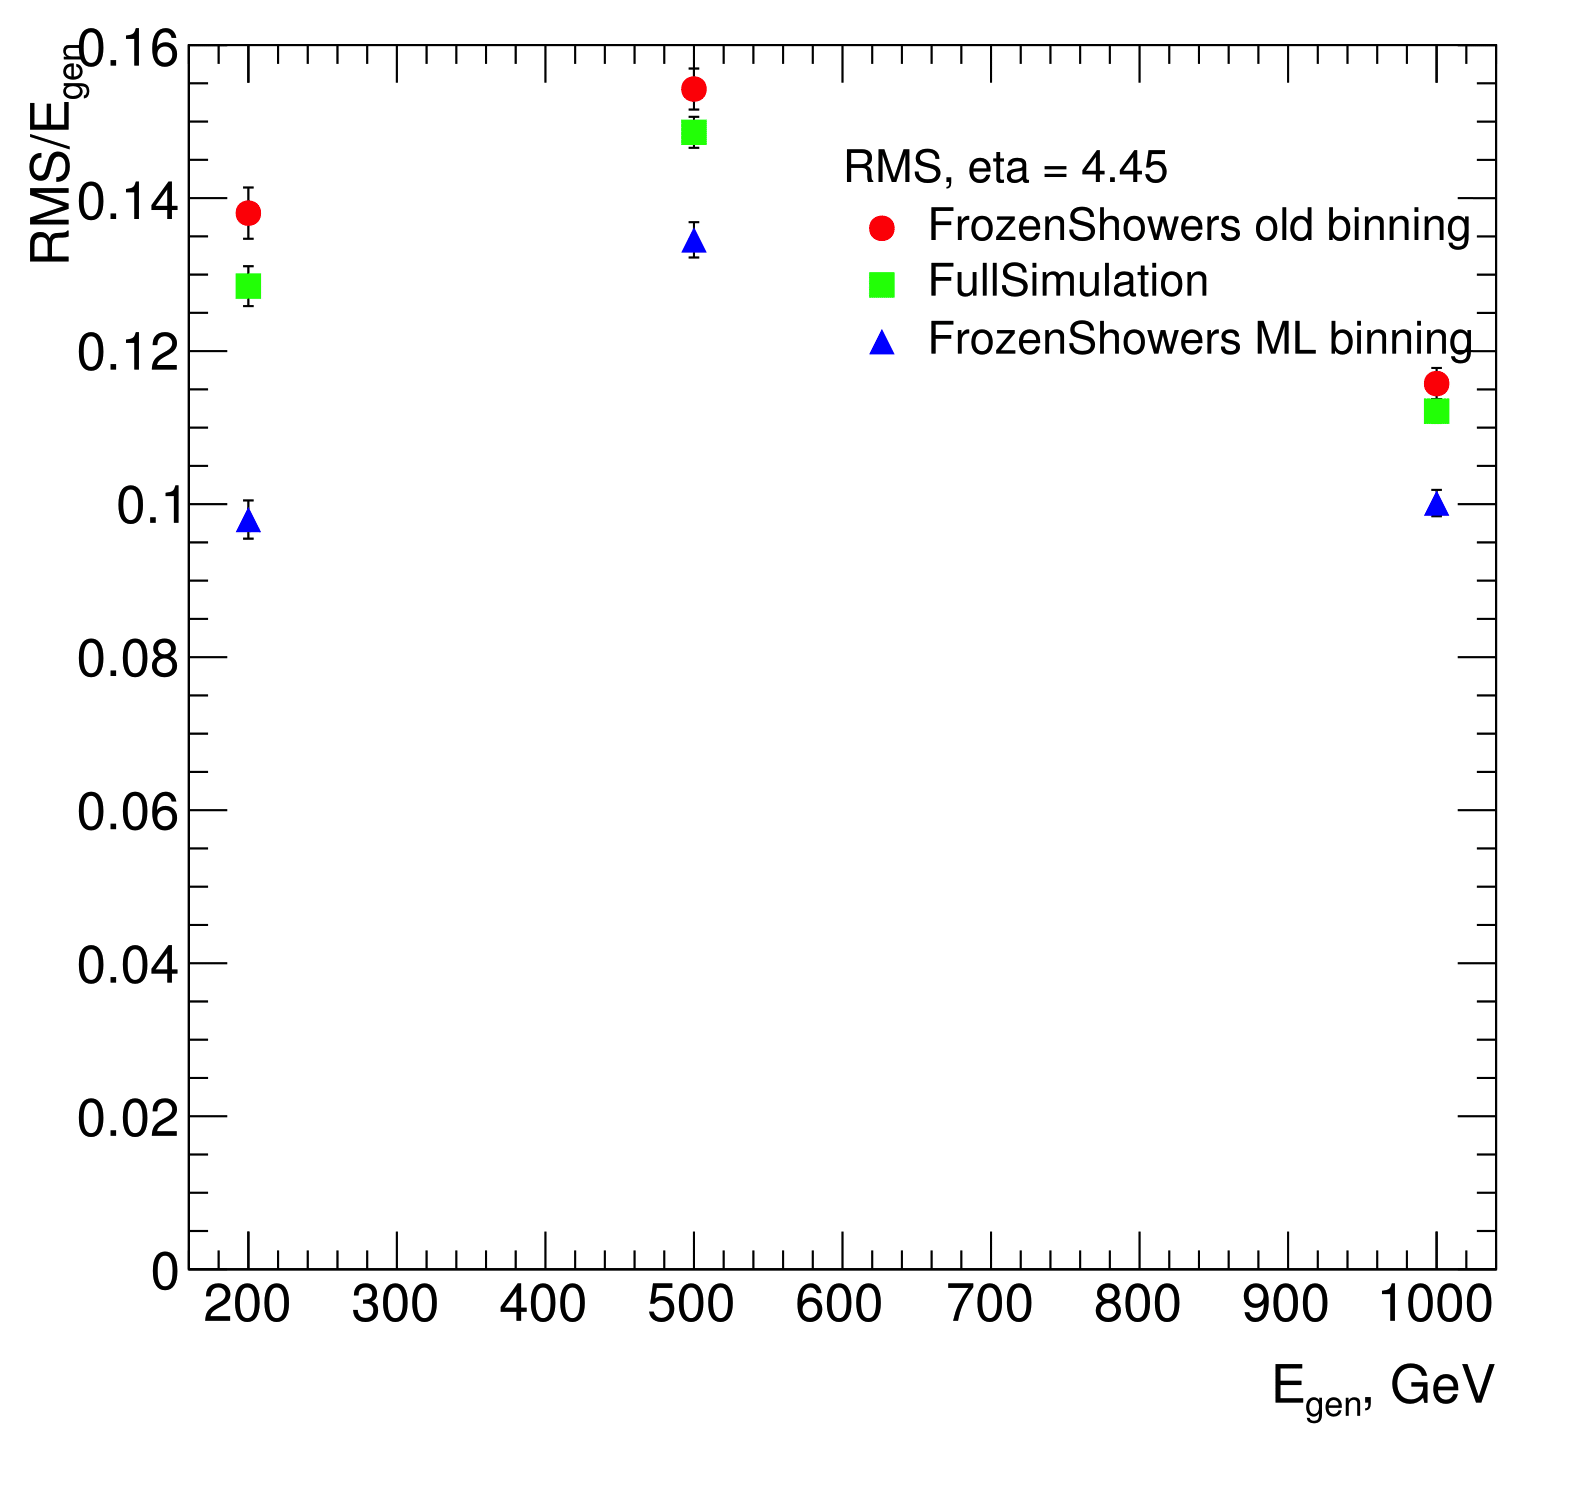
\includegraphics[width=1.\linewidth]{MC/RMS/RMS-02.png} }
\end{minipage}
\hfill
\begin{minipage}[h]{0.32\linewidth}
\center{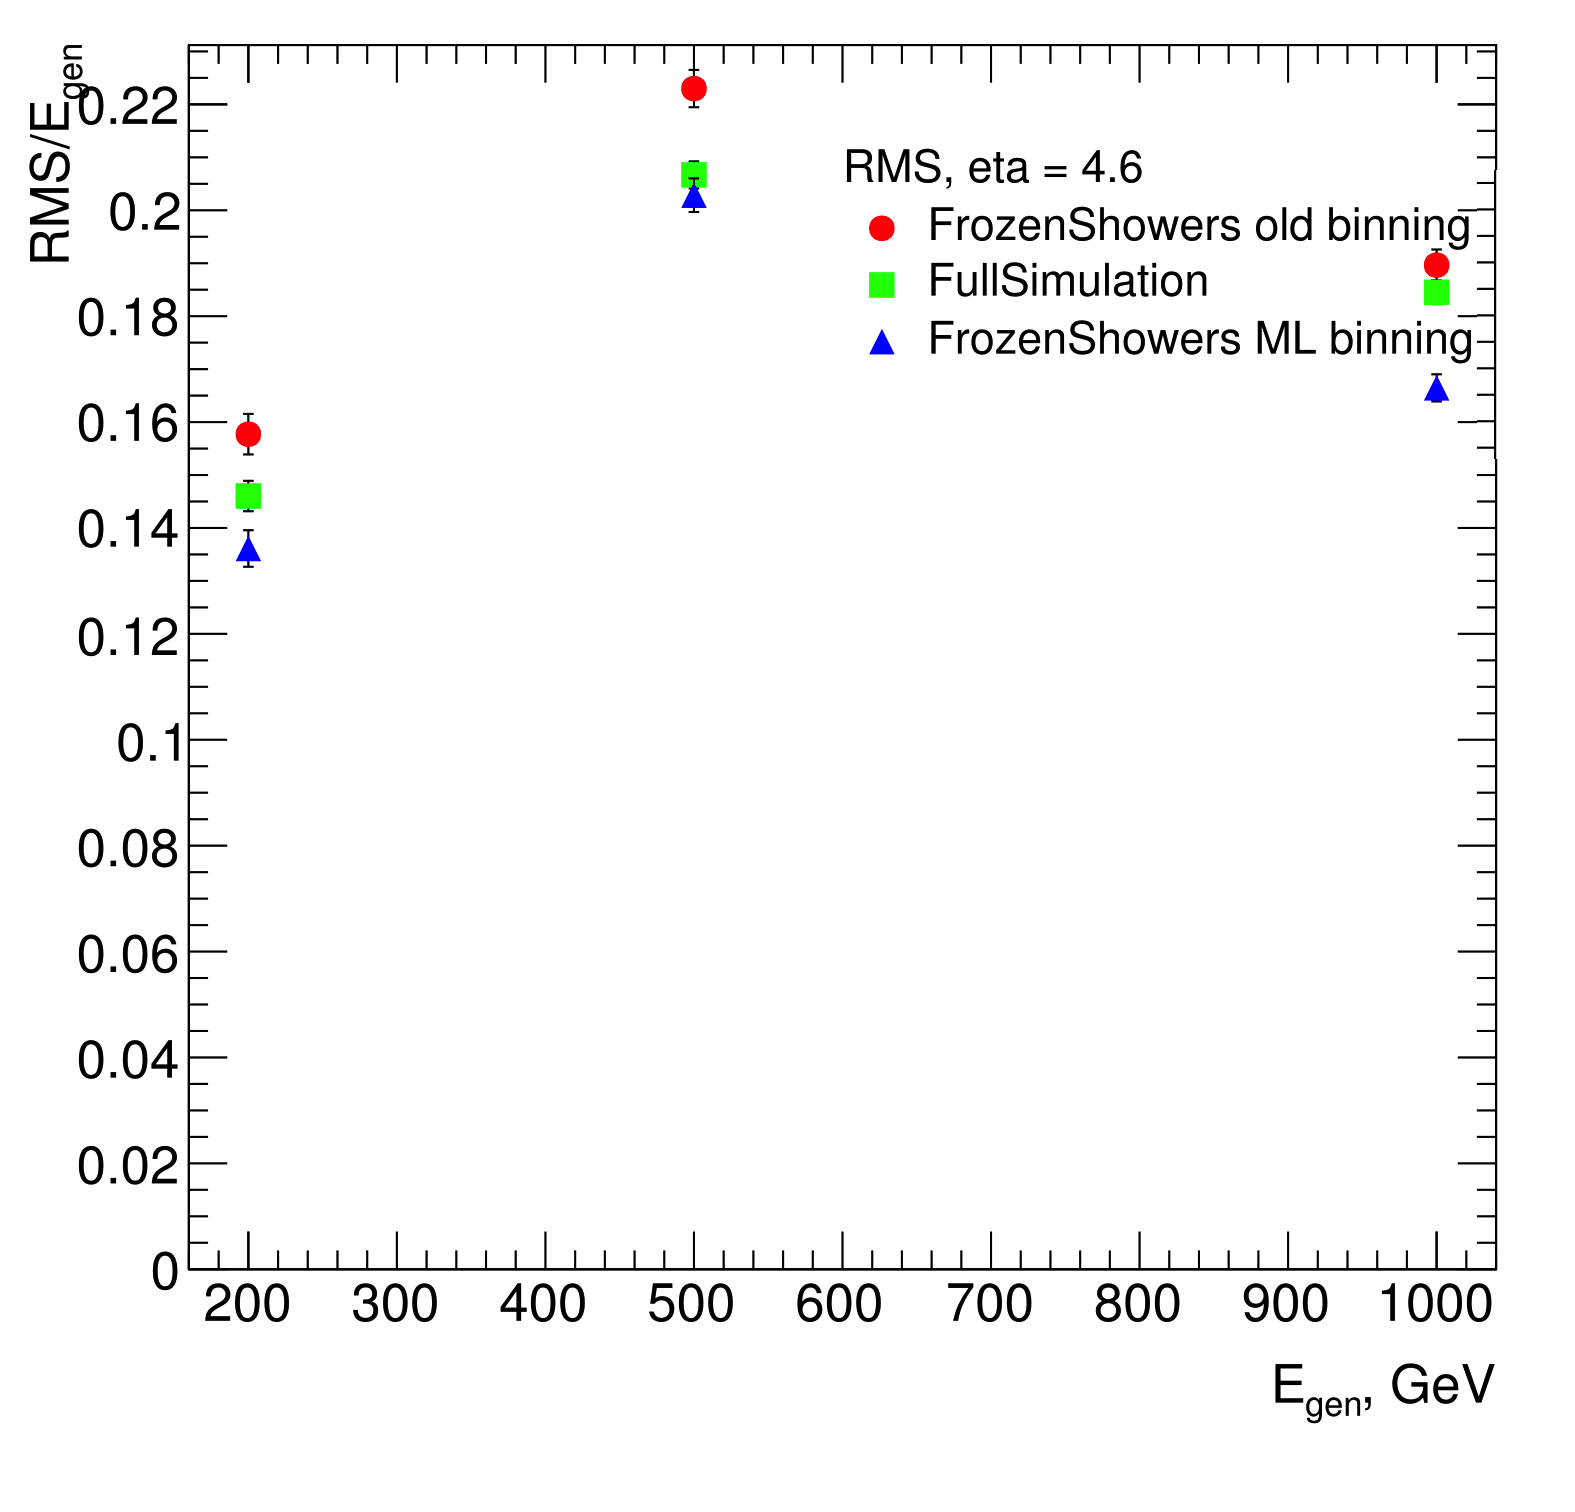
\includegraphics[width=1.\linewidth]{MC/RMS/RMS-01.png} }
\end{minipage}
\caption{Energy resolution of reconstructed electrons for full simulation, new libraries with ML binning and old tuned libraries with original binning for different $\eta$ bins }
\label{fig:Reso}
\end{figure}

\begin{figure}[!tbp]
\begin{minipage}[h]{0.32\linewidth}
\center{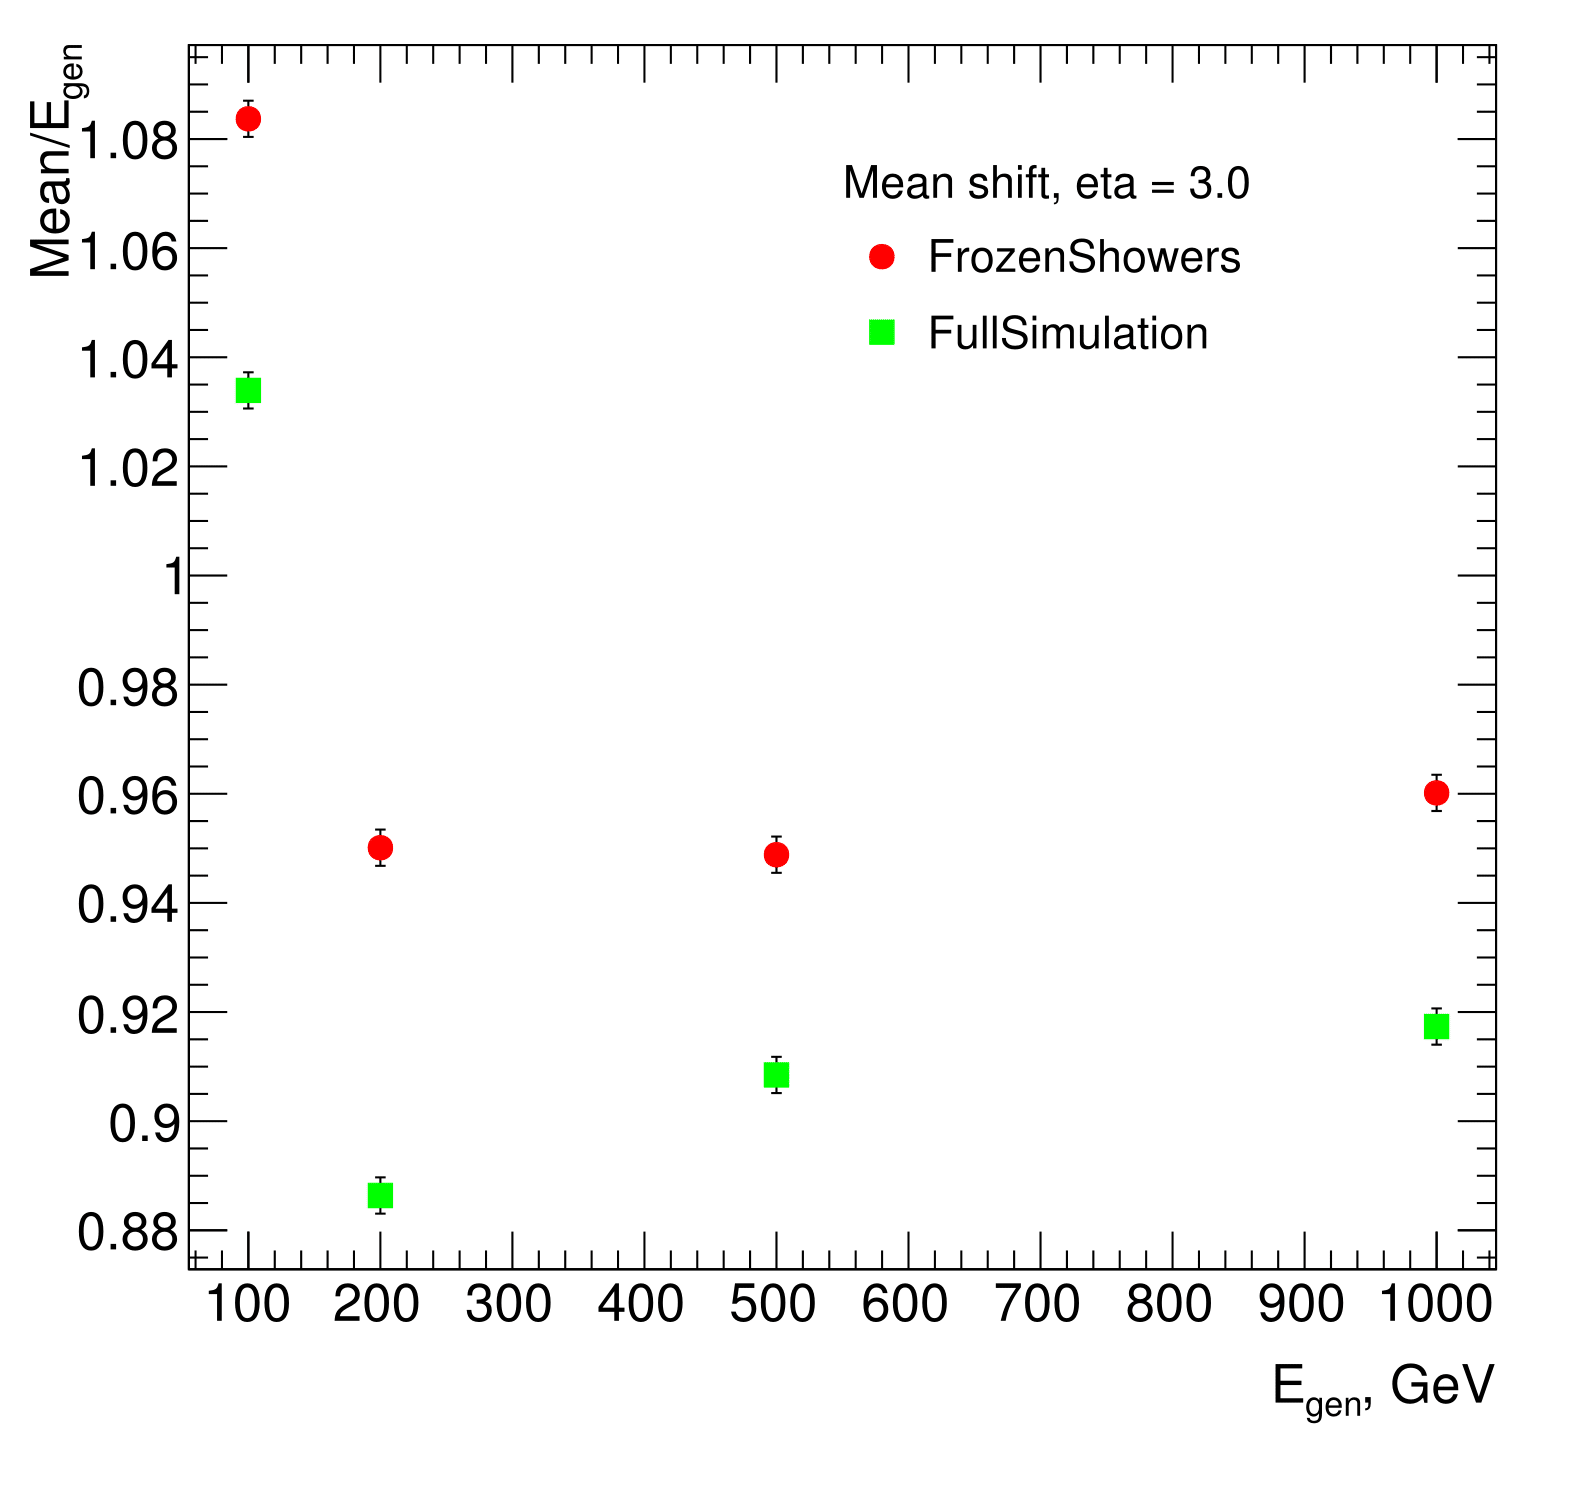
\includegraphics[width=1.\linewidth]{MC/Mean/Mean-12.png} }
\end{minipage}
\hfill
\begin{minipage}[h]{0.32\linewidth}
\center{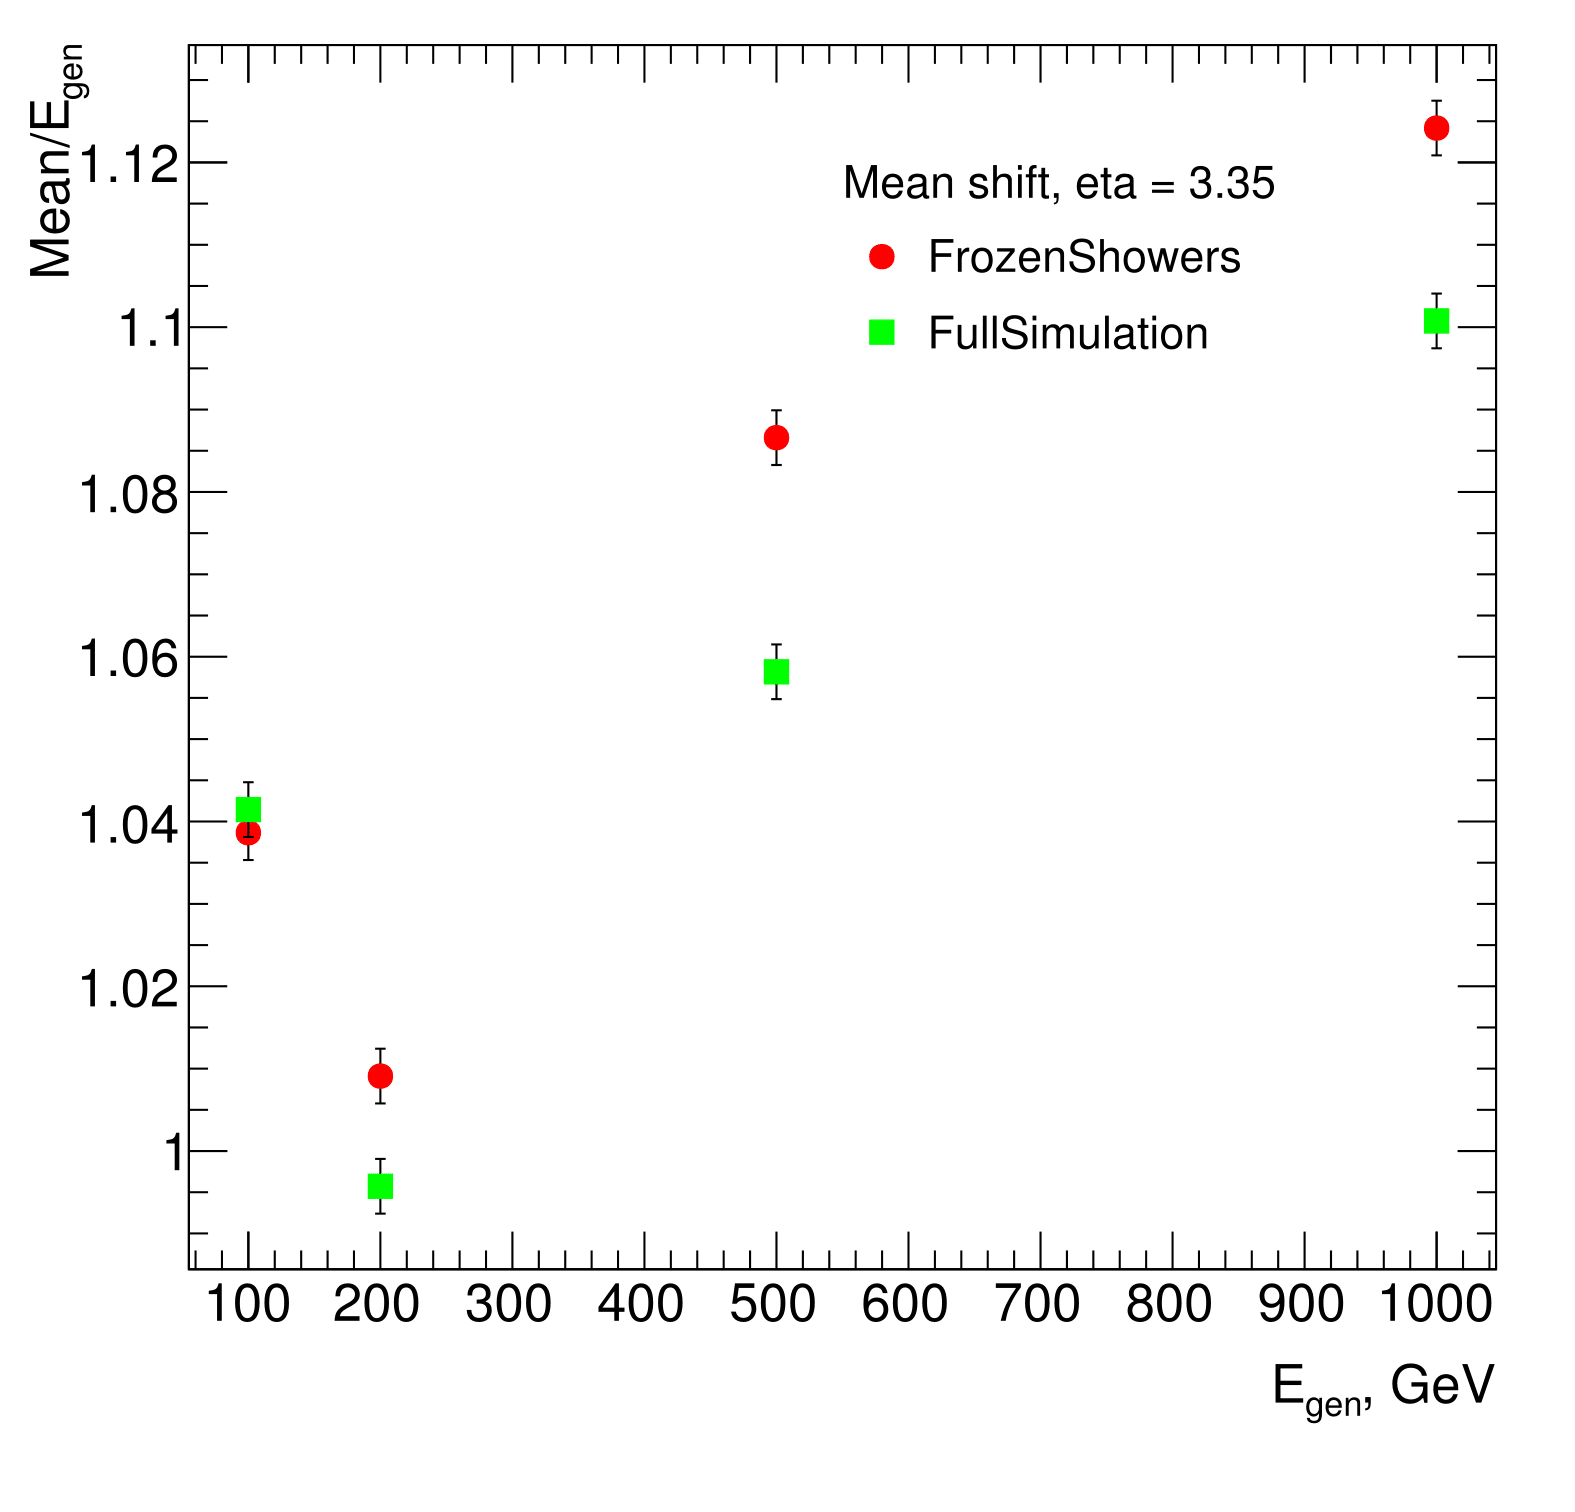
\includegraphics[width=1.\linewidth]{MC/Mean/Mean-11.png}  }
\end{minipage}
\hfill
\begin{minipage}[h]{0.32\linewidth}
\center{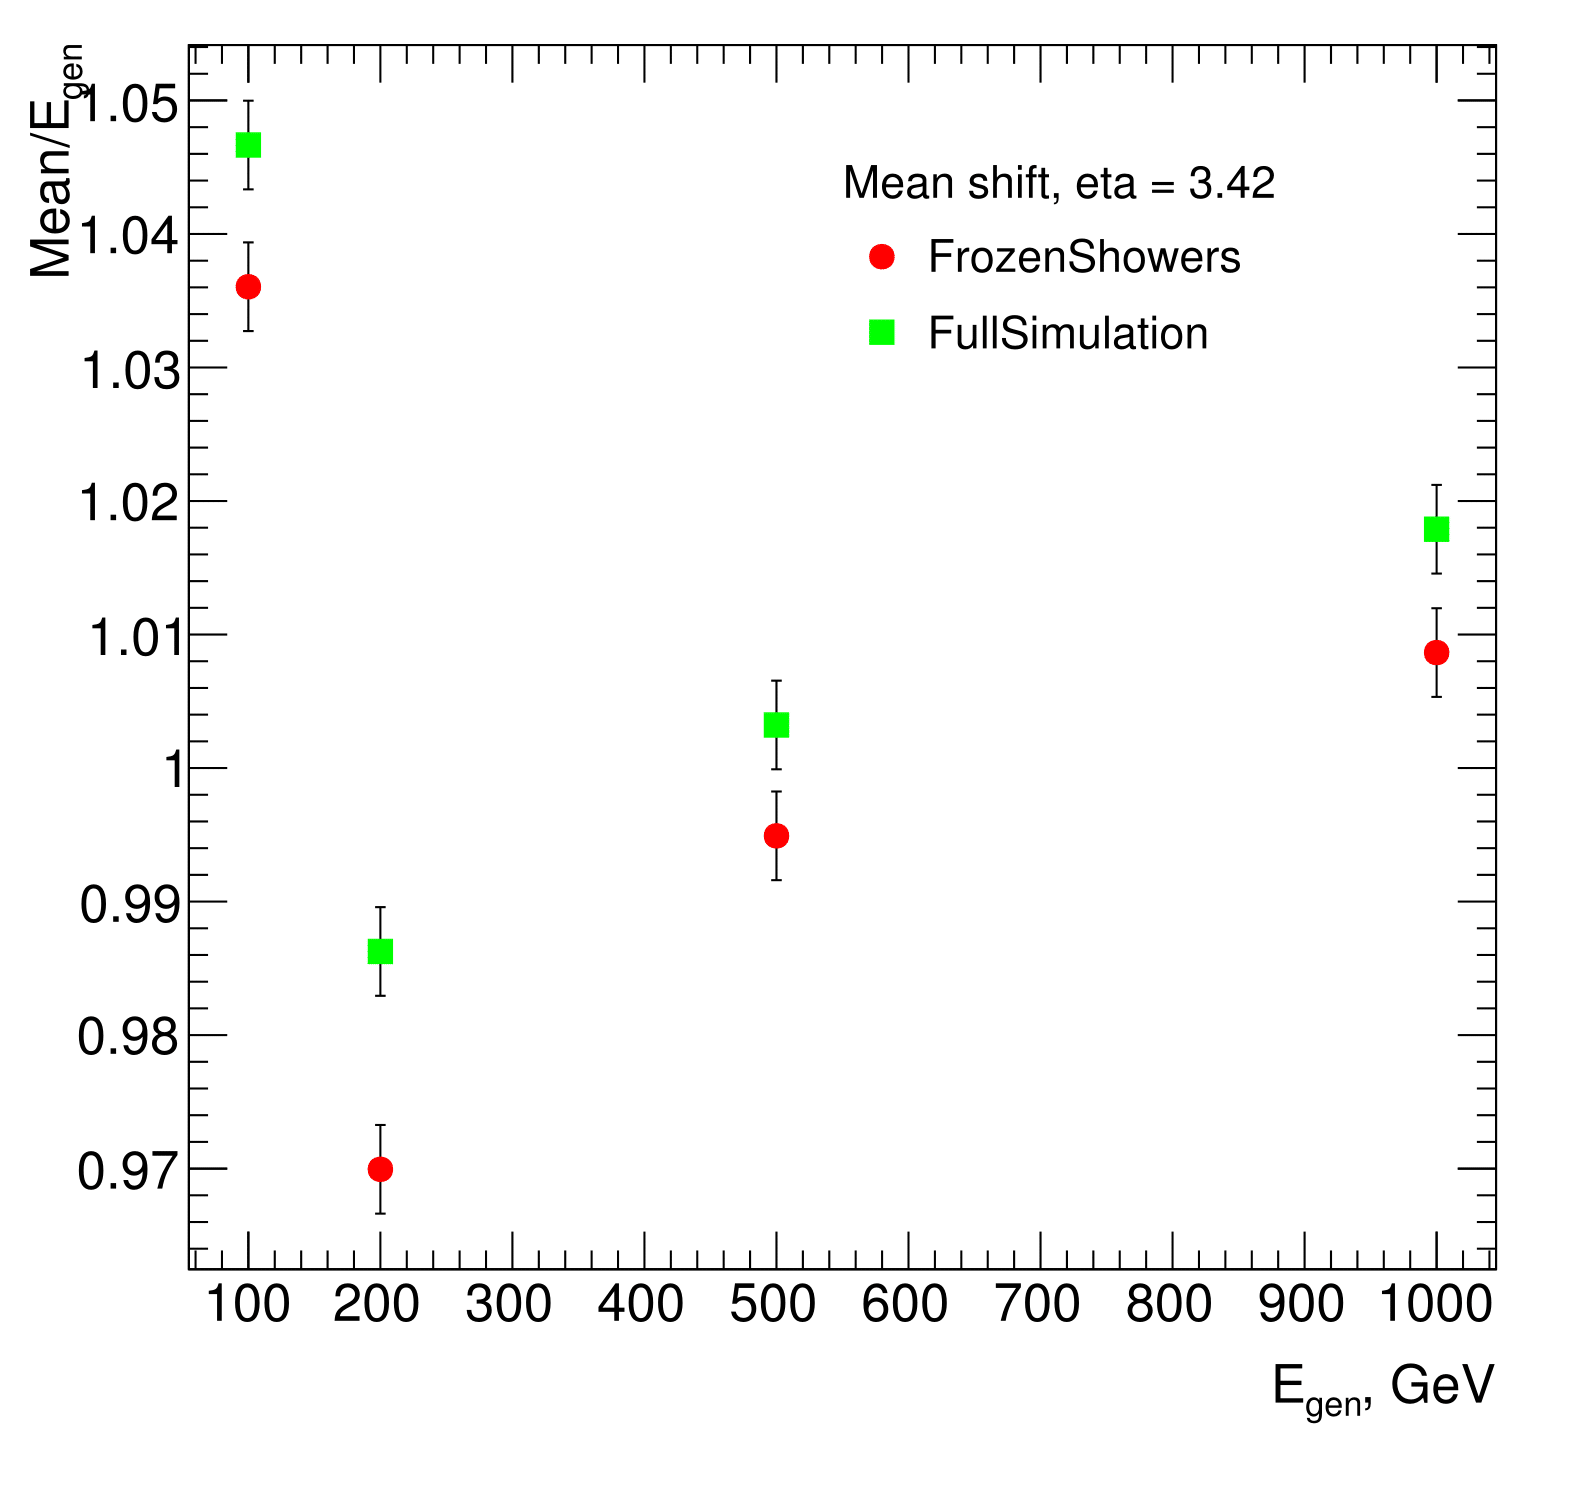
\includegraphics[width=1.\linewidth]{MC/Mean/Mean-10.png}  }
\end{minipage}
\vfill
\begin{minipage}[h]{0.32\linewidth}
\center{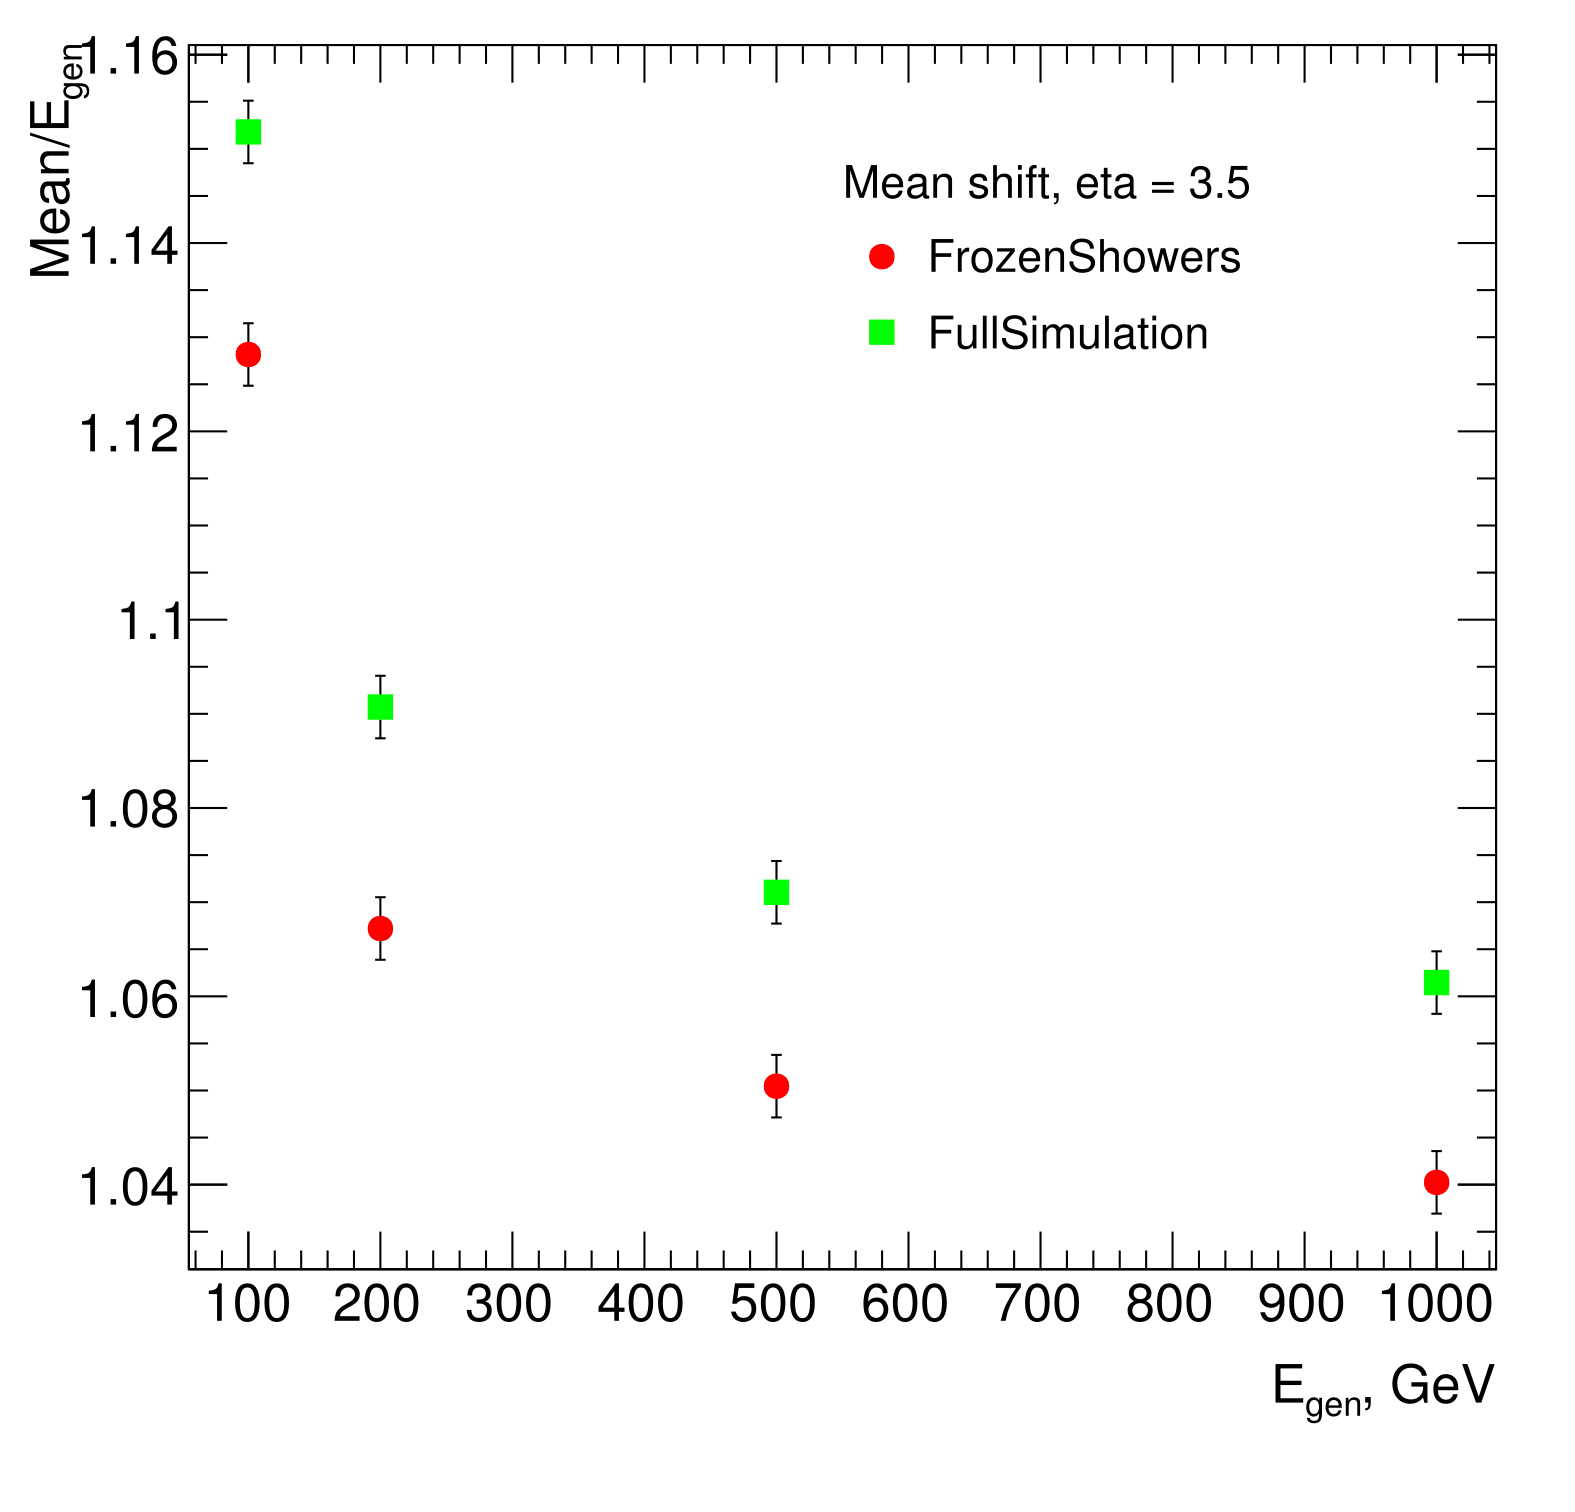
\includegraphics[width=1.\linewidth]{MC/Mean/Mean-09.png}  }
\end{minipage}
\hfill
\begin{minipage}[h]{0.32\linewidth}
\center{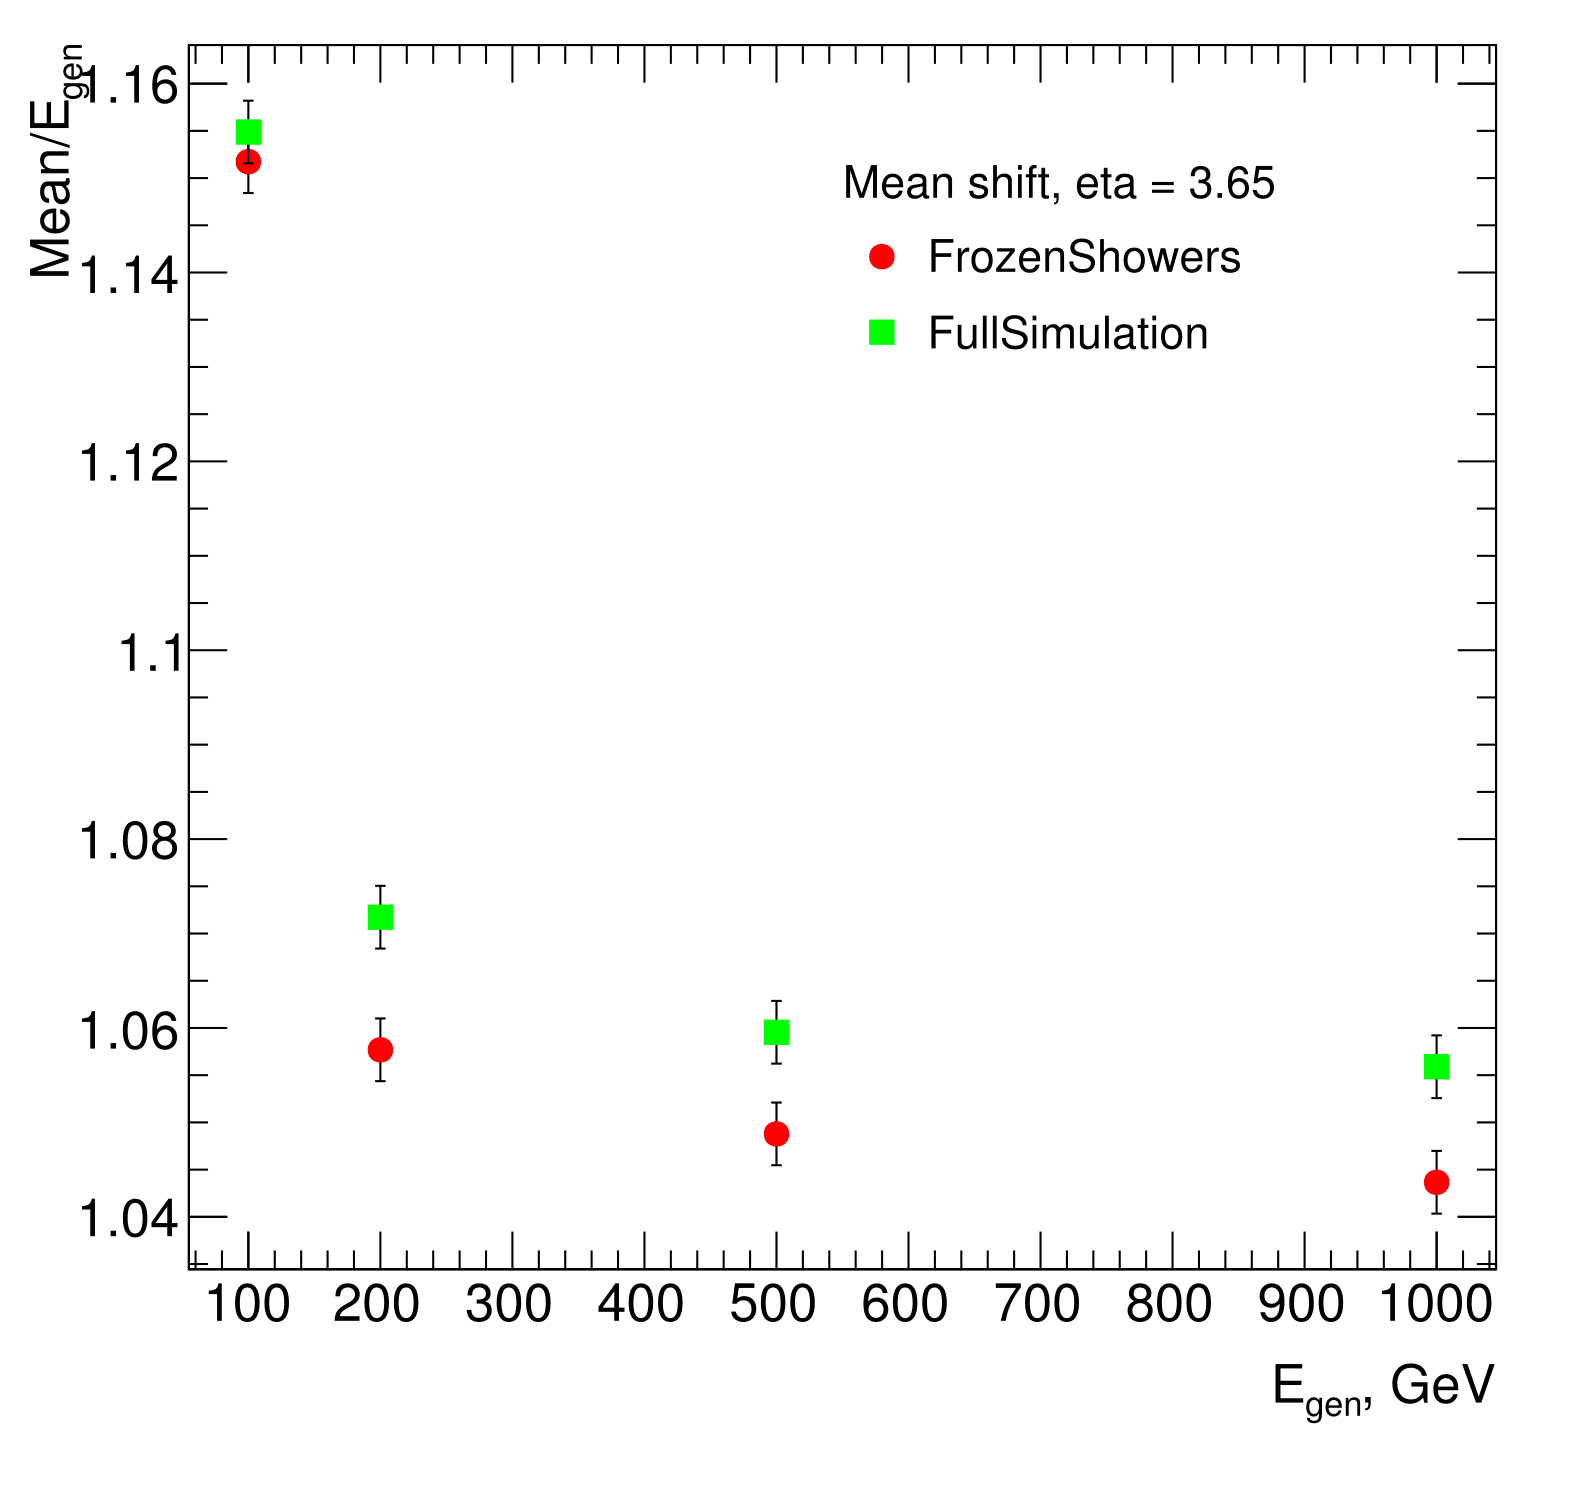
\includegraphics[width=1.\linewidth]{MC/Mean/Mean-08.png}  }
\end{minipage}
\hfill
\begin{minipage}[h]{0.32\linewidth}
\center{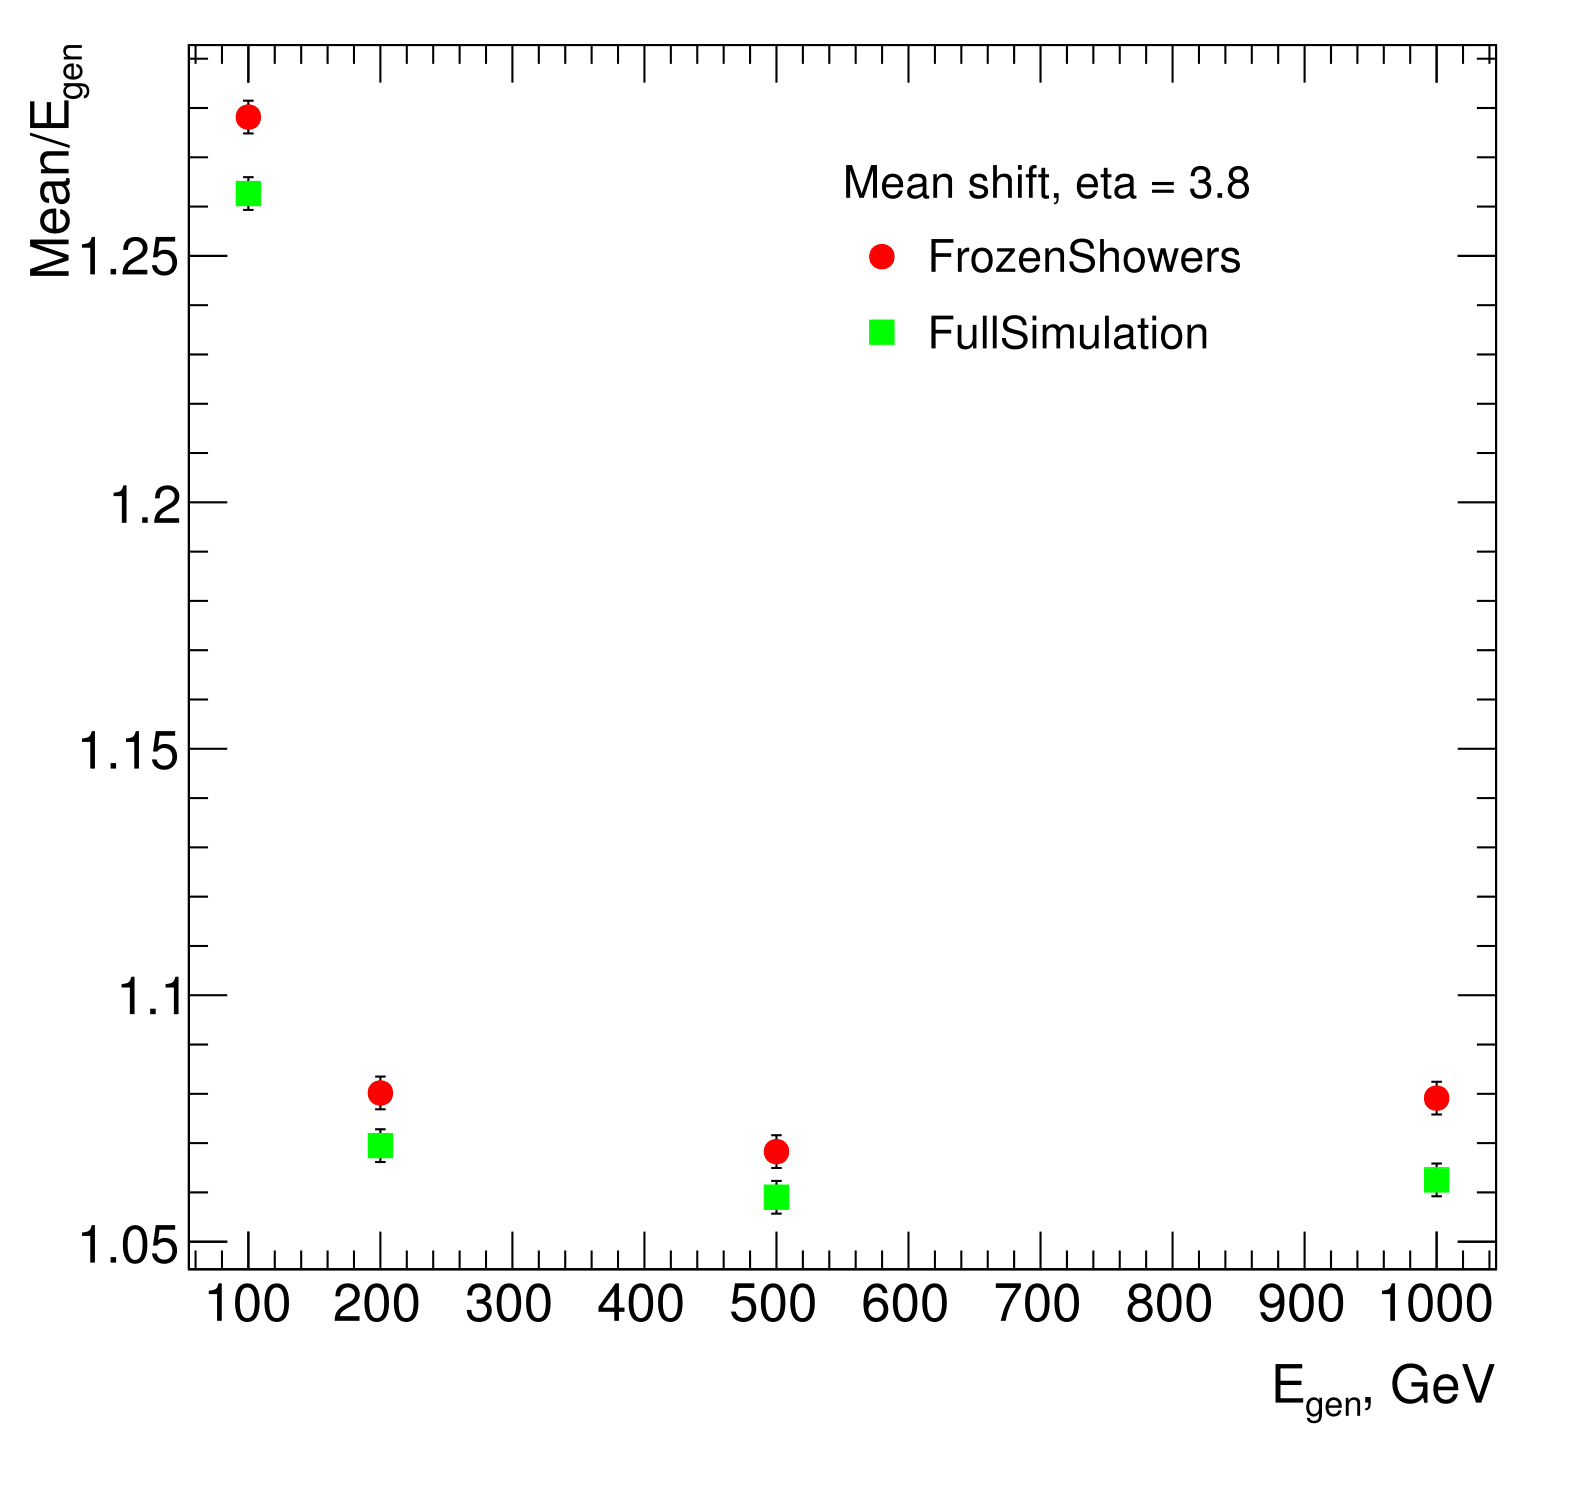
\includegraphics[width=1.\linewidth]{MC/Mean/Mean-07.png}  }
\end{minipage}
\vfill
\begin{minipage}[h]{0.32\linewidth}
\center{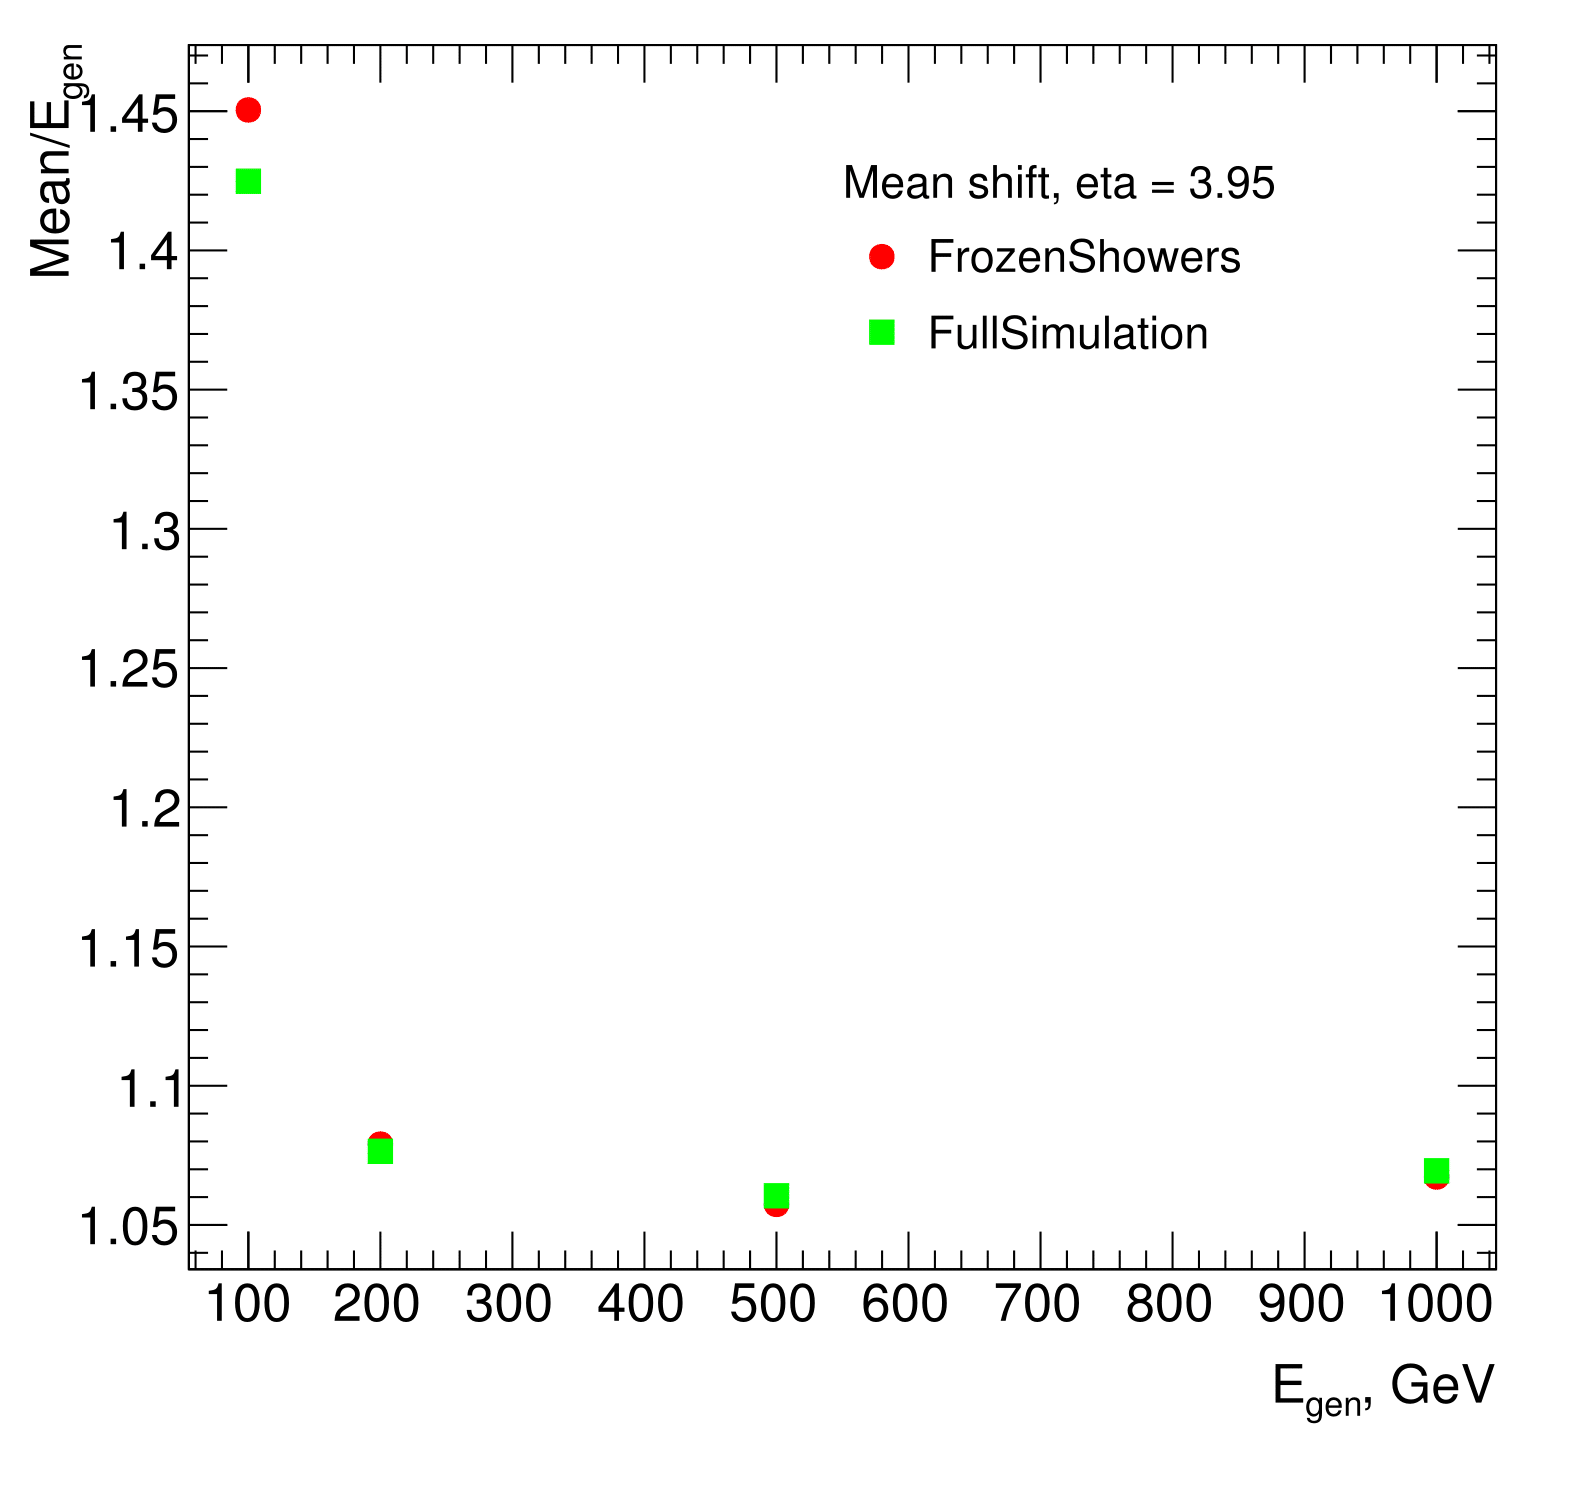
\includegraphics[width=1.\linewidth]{MC/Mean/Mean-06.png}  }
\end{minipage}
\hfill
\begin{minipage}[h]{0.32\linewidth}
\center{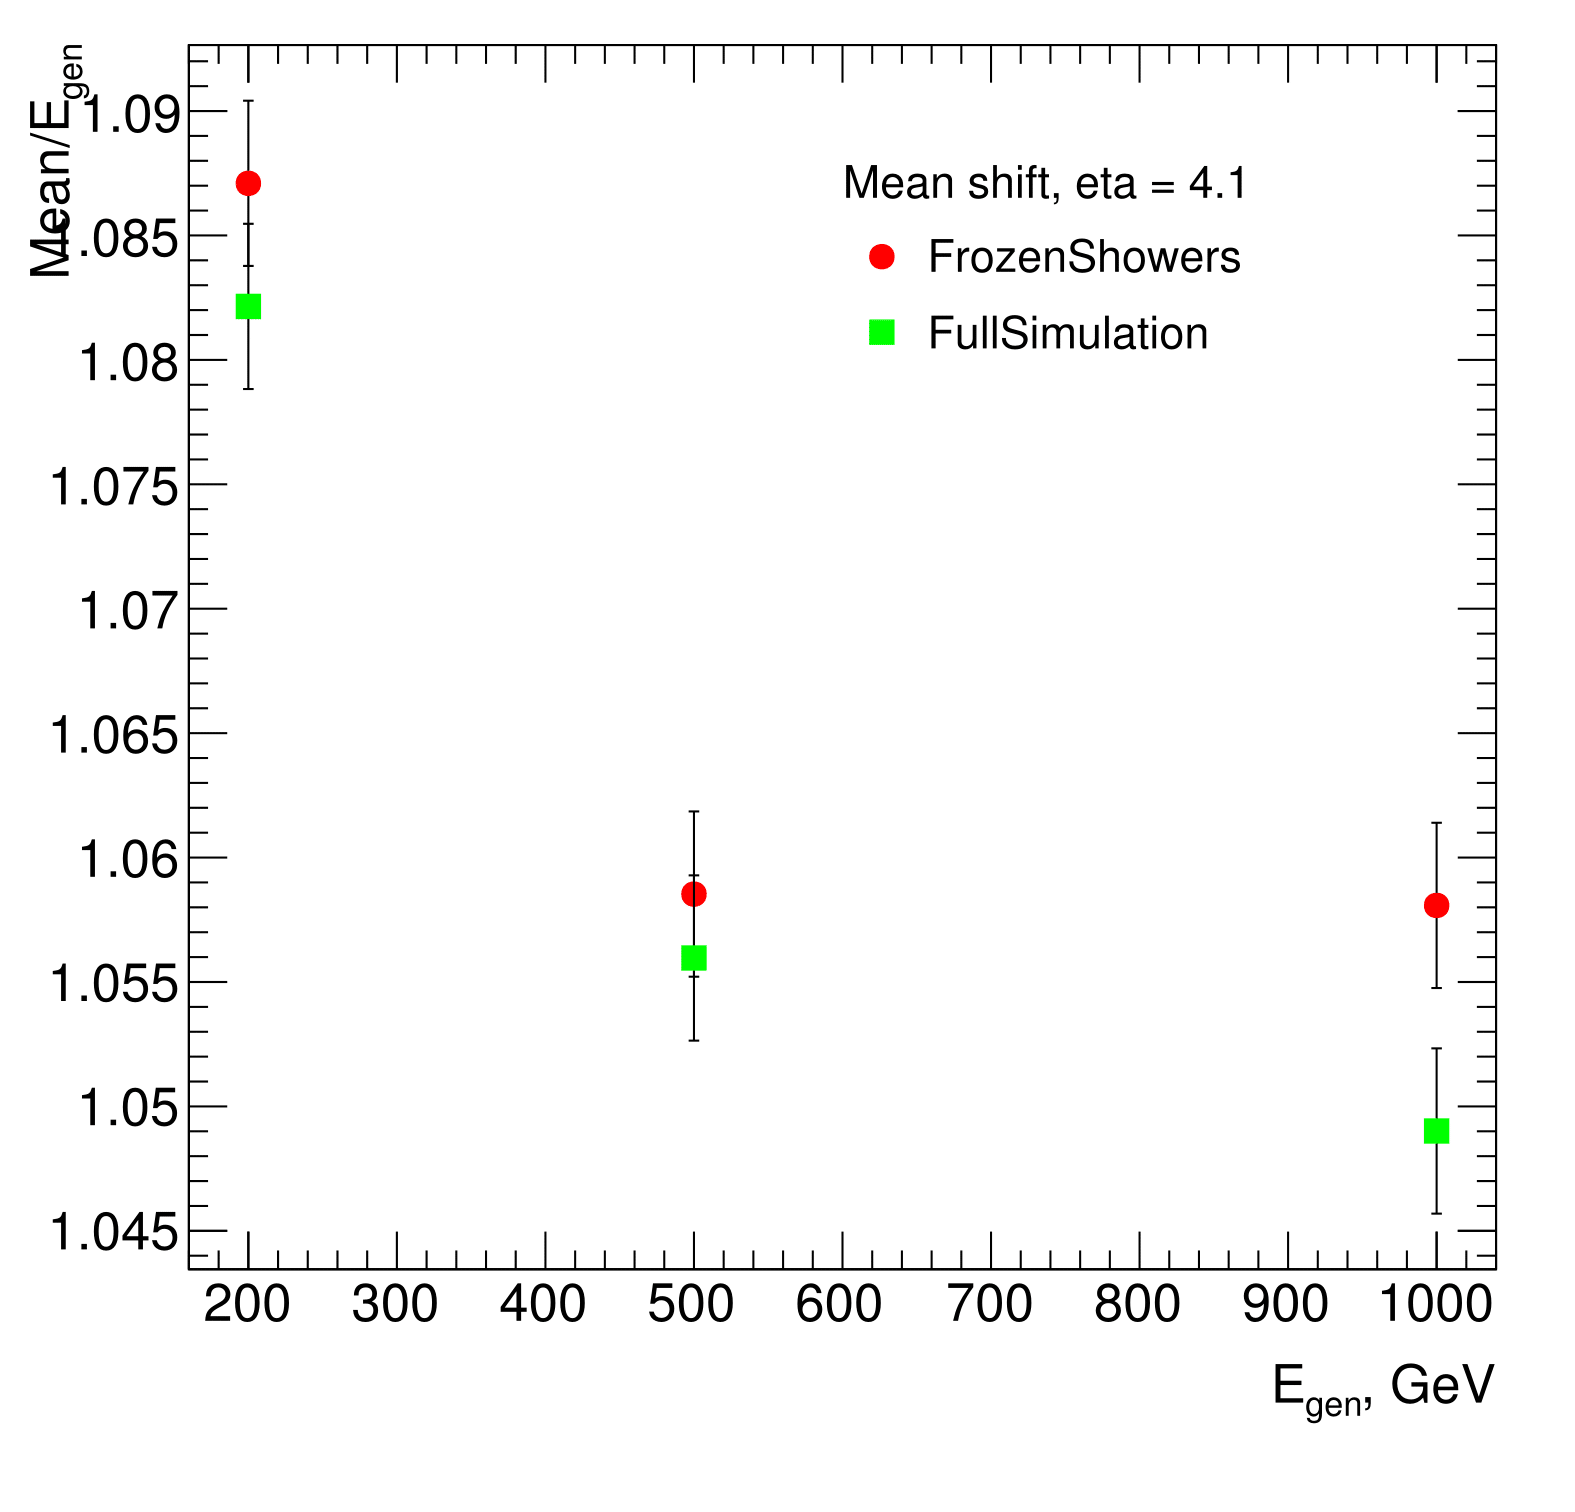
\includegraphics[width=1.\linewidth]{MC/Mean/Mean-05.png}  }
\end{minipage}
\hfill
\begin{minipage}[h]{0.32\linewidth}
\center{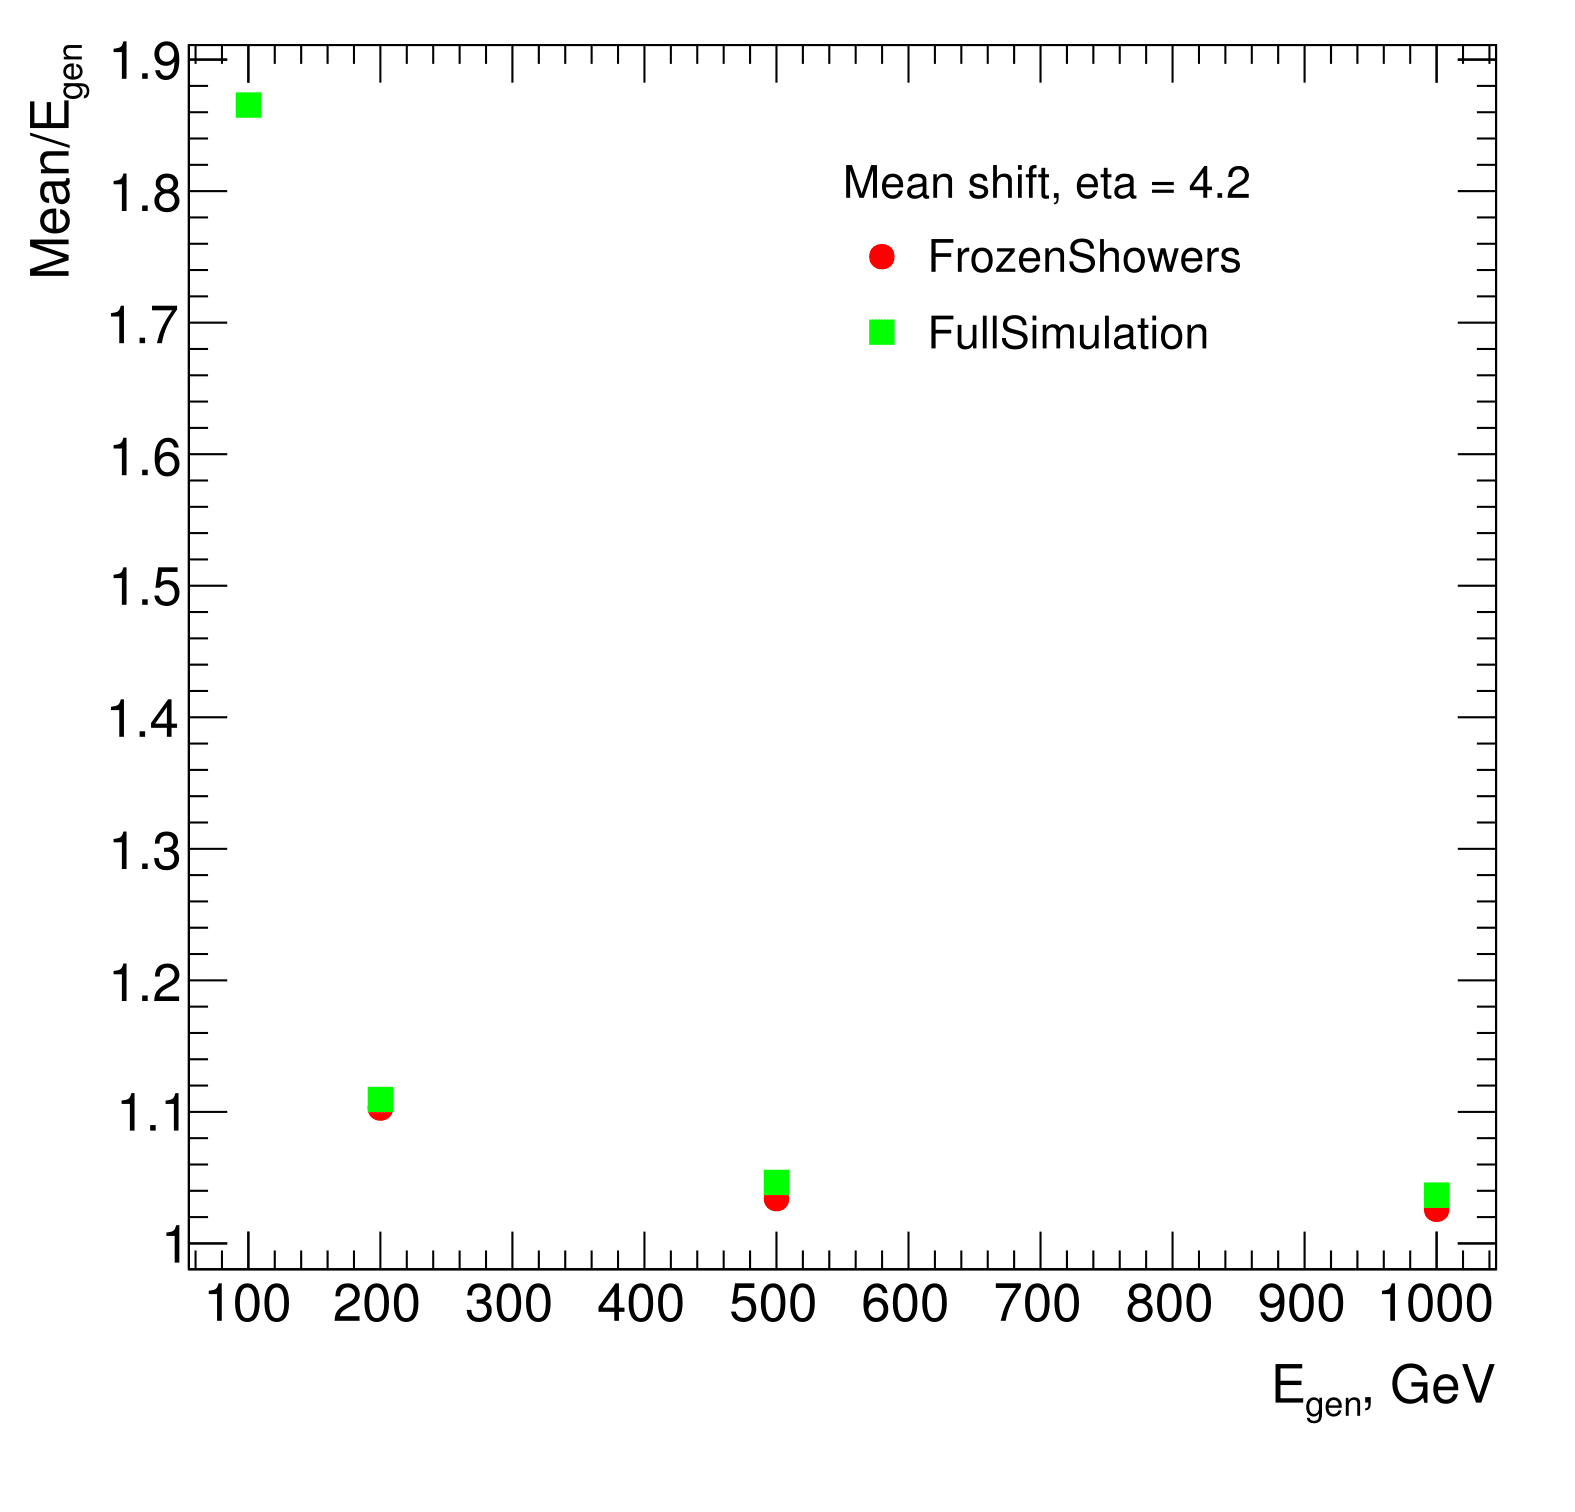
\includegraphics[width=1.\linewidth]{MC/Mean/Mean-04.png}  }
\end{minipage}
\vfill
\begin{minipage}[h]{0.32\linewidth}
\center{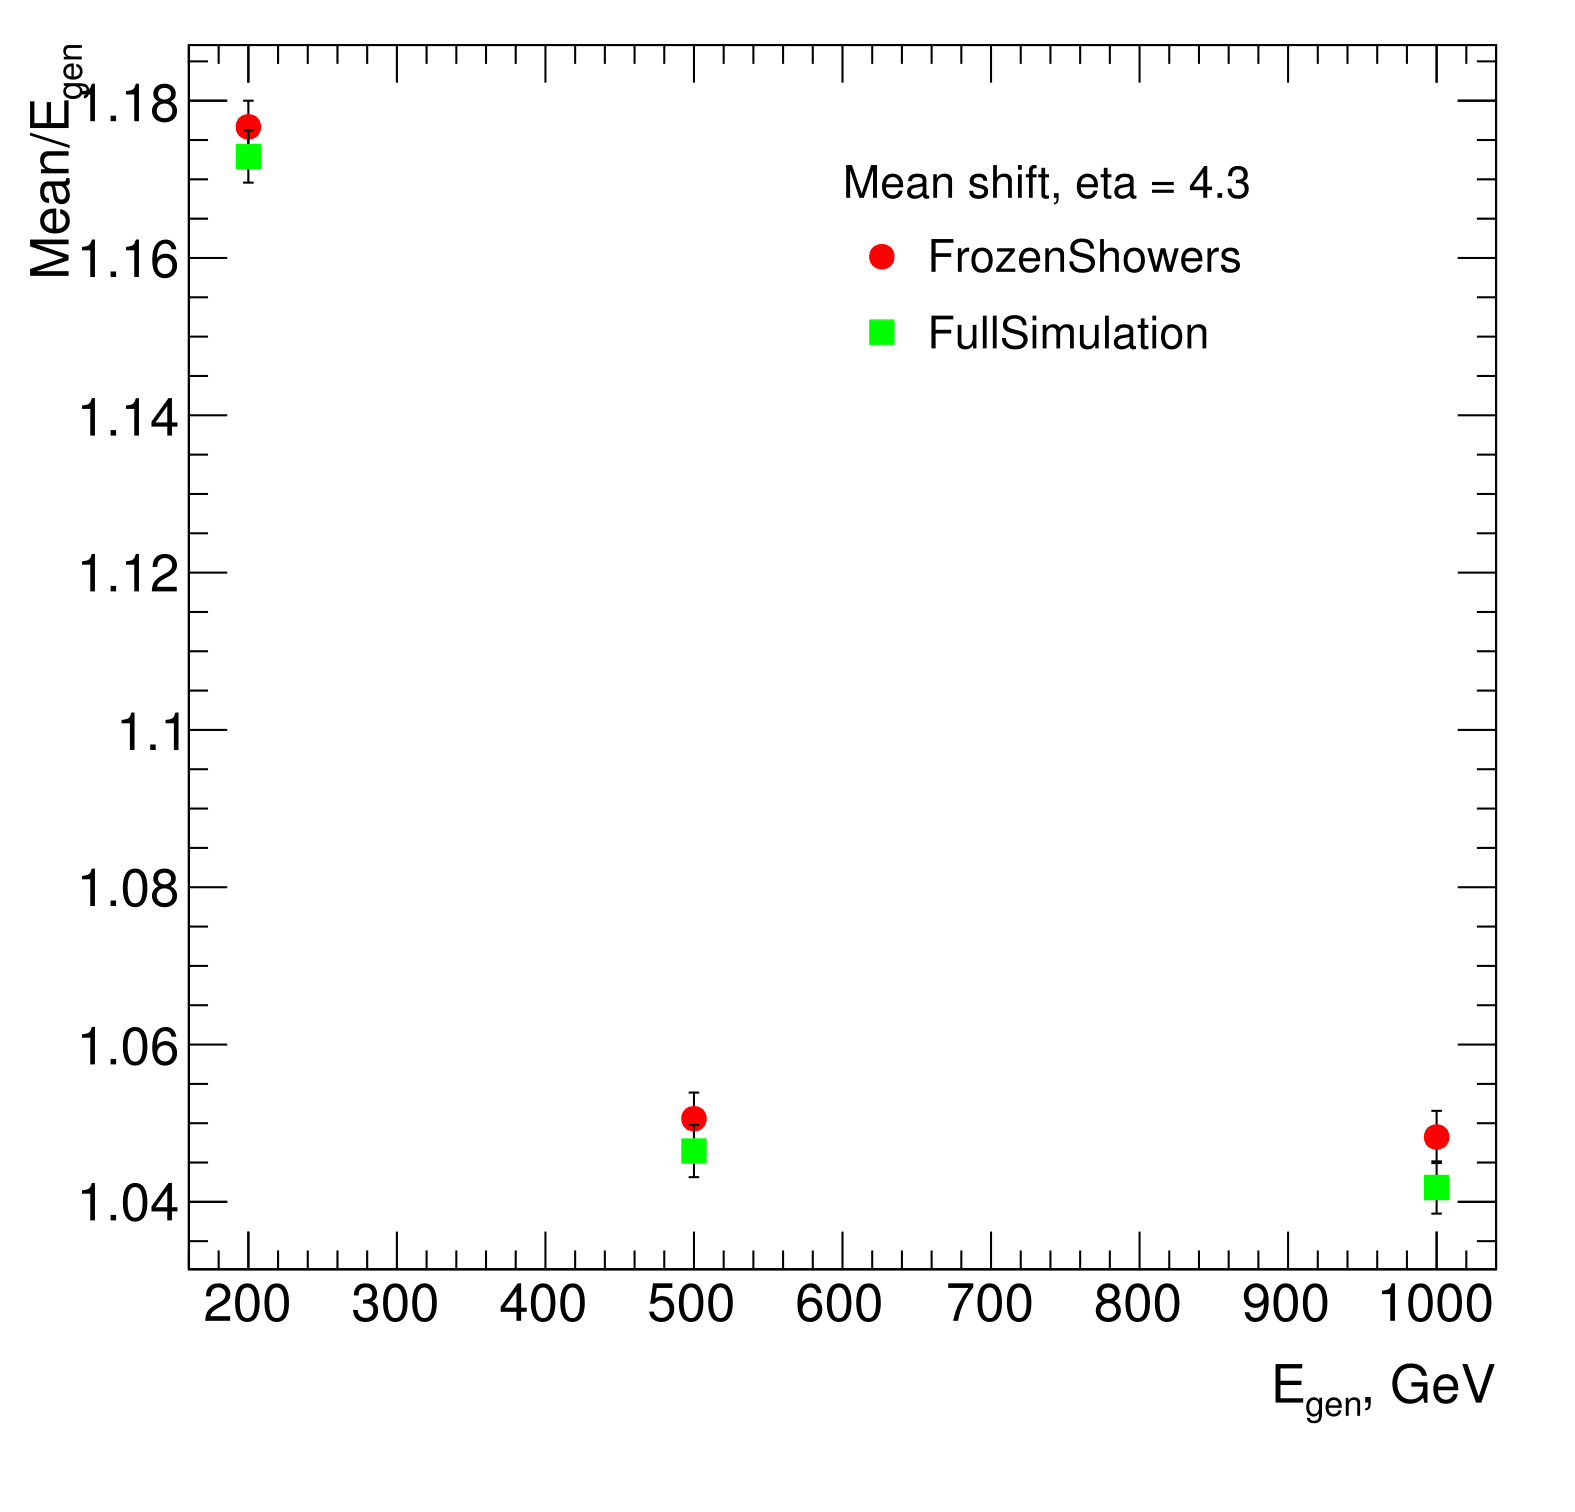
\includegraphics[width=1.\linewidth]{MC/Mean/Mean-03.png}  }
\end{minipage}
\hfill
\begin{minipage}[h]{0.32\linewidth}
\center{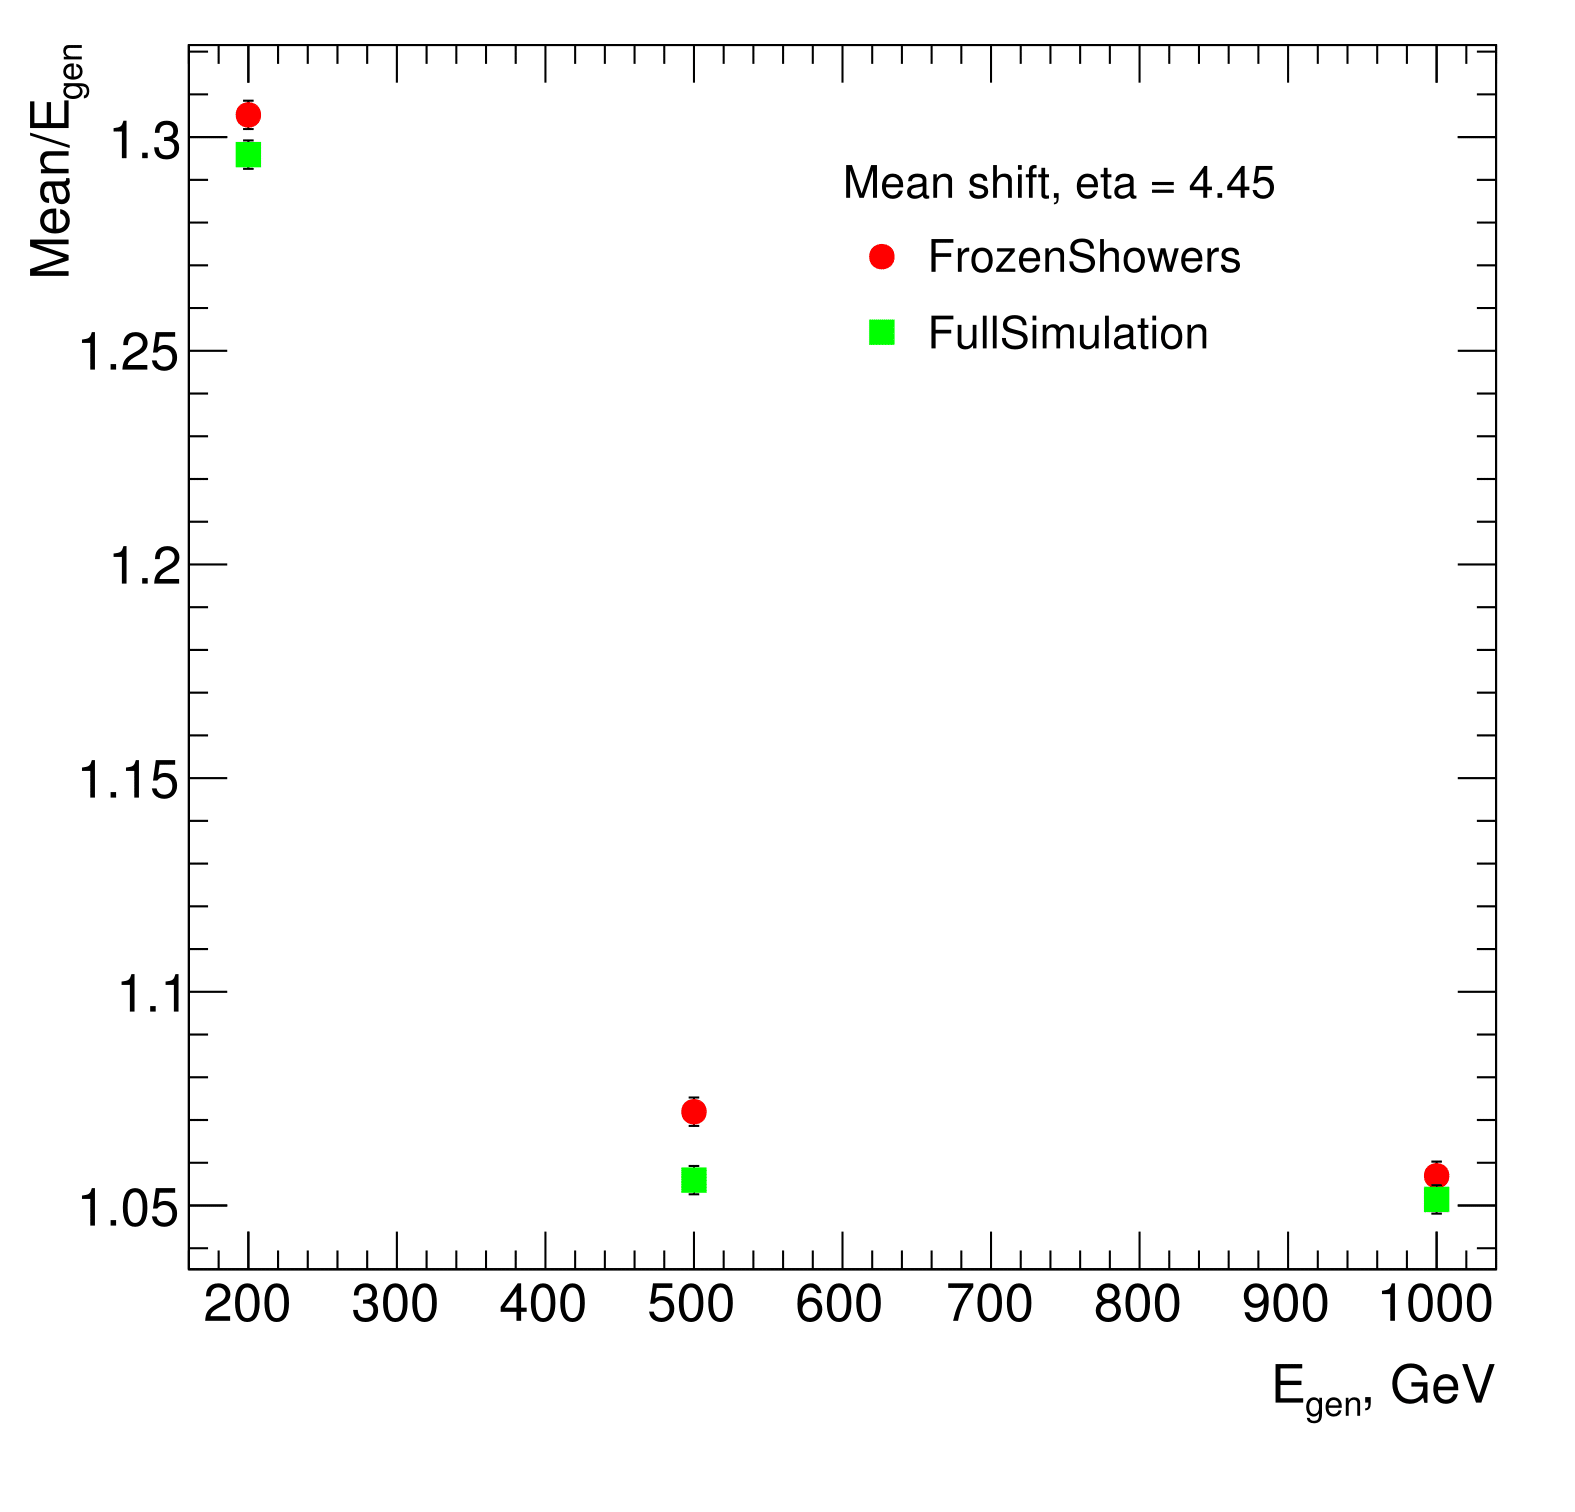
\includegraphics[width=1.\linewidth]{MC/Mean/Mean-02.png}  }
\end{minipage}
\hfill
\begin{minipage}[h]{0.32\linewidth}
\center{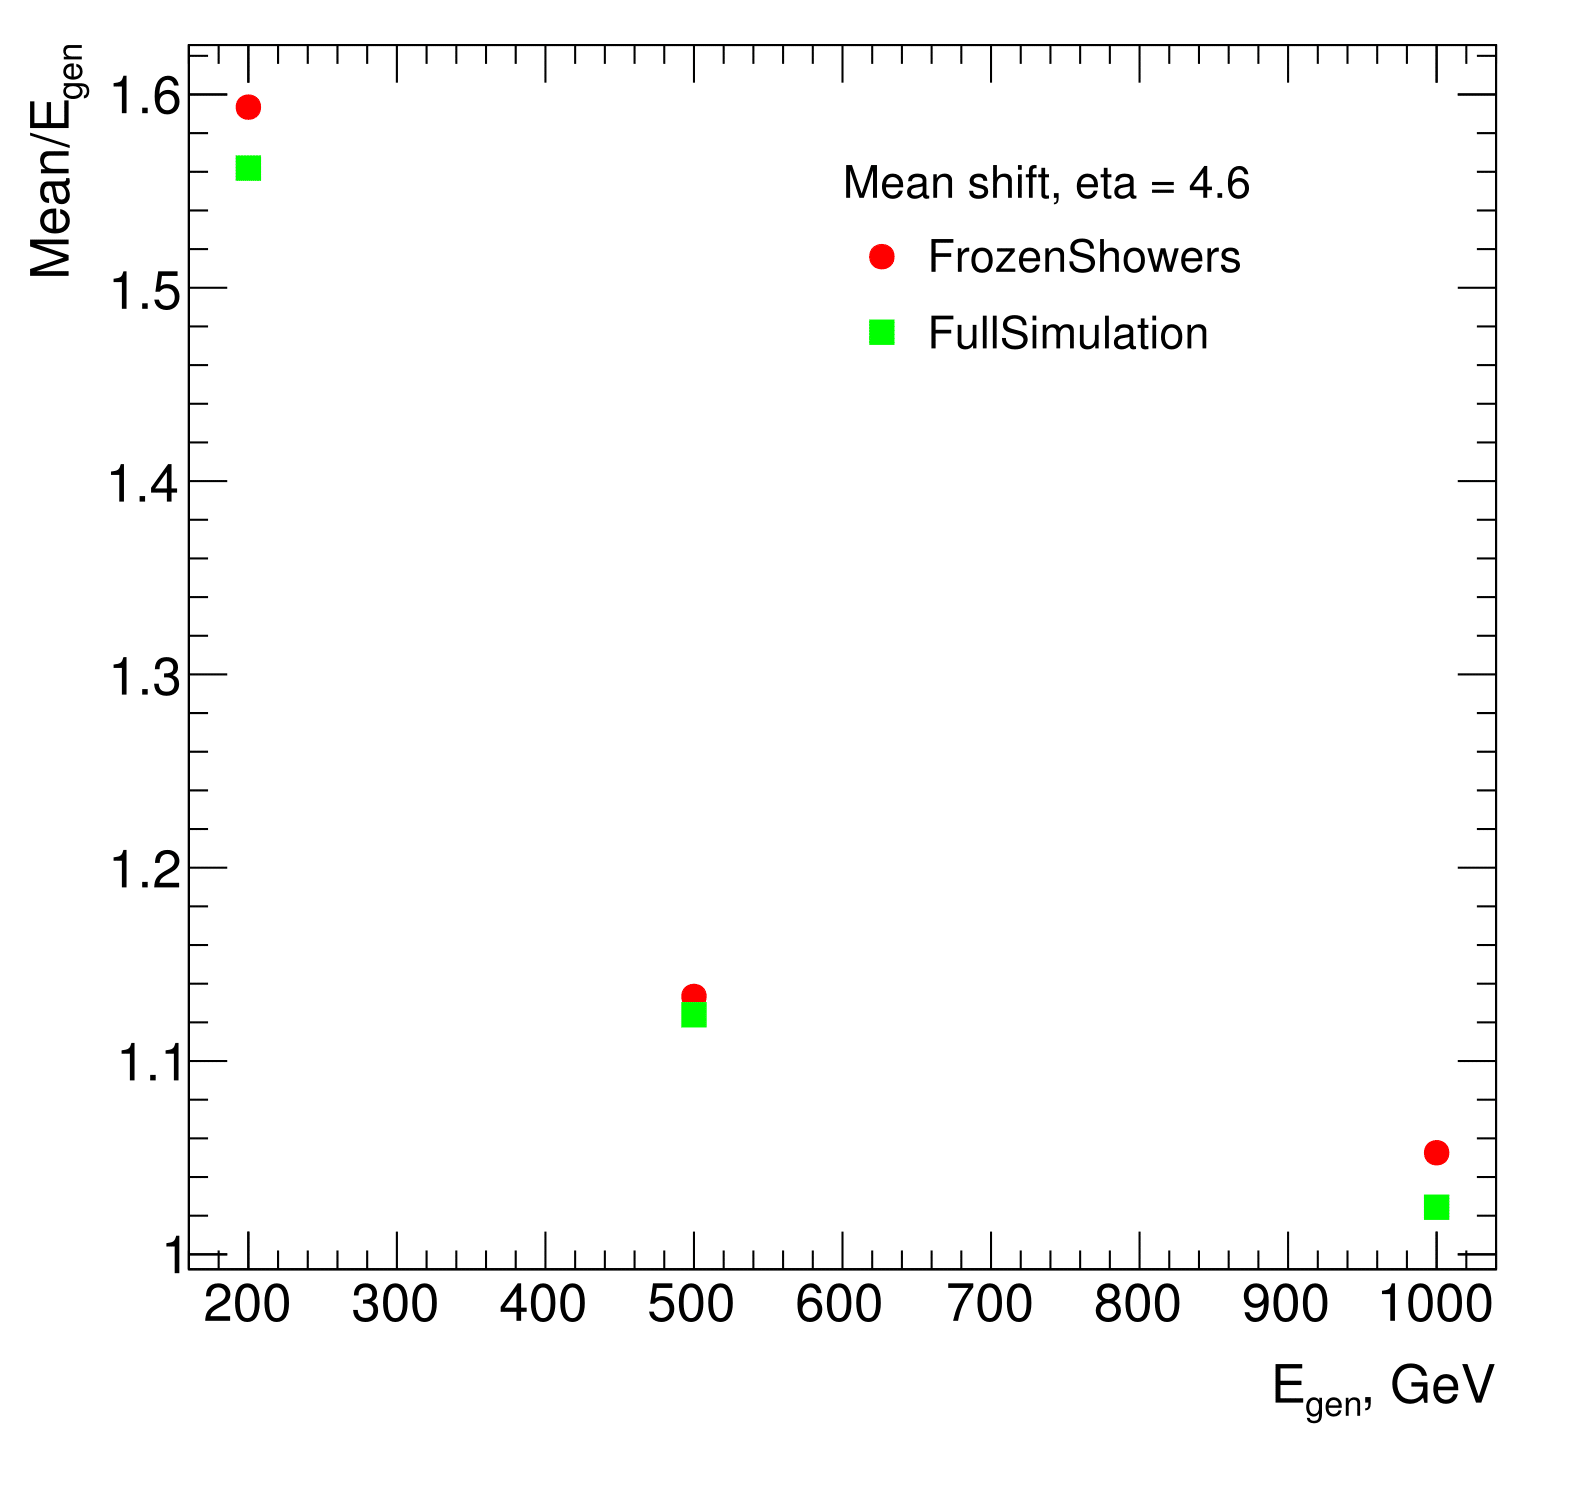
\includegraphics[width=1.\linewidth]{MC/Mean/Mean-01.png}  }
\end{minipage}
\caption{Shift of the reconstructed energy to the truth energy of electrons for full simulation, new FS libraries with ML binning and full simulation for different $\eta$ bins }
\label{fig:Mean}
\end{figure}

\subsection{Plans for the future}\label{sec:FSImpr}

The validation have showed a good agrement between full simulation and fast simulation for most of the bins, however, because not all of the bins are performing equally well, the additional modifications of the algorithm are needed. The following modifications have been investigated and planned to be performed in the nearest future:
\begin{itemize}
\item Procedure with $\eta$ dependent bin size. Currently all of the bins have the same size and position of the liquid argon bin. However, because of the outlying bins, the procedure should be modified and determine the bin position separately for each bin.
\item Use of the closer to real case for training sample. The problem of electron resolution could be also caused by too simlified models, used to train on. It is planned to repeat the procedure for training sample with distributions, closer to the nominal ones.
\item Adding the direction of the shower binned variable. Since there is a complicated dependency between position of the electron and its direction (especially in small energy region), the additional binning could solve the remaining problems with electron energy resolution.
\item Replacing distance to the closest rod binning by approximate path in the liquid argon. 
\end{itemize}

\section{Validation of the new libraries}\label{sec:FSValidation}

The good fast simulation method should work equally good on all types of reconstructed objects, this is why for each new frozen showers libraries production an new iteration of mass validation is performed. The validation is done separately for each object by the different groups by comparing the distibutions obtained from full and fast simulation

Frozen showers have been validated on following objects and showed a good agreement:
\begin{itemize}
\item Z bosons from $Z \to ee$ sample with one central and one forward electrons(Fig. \ref{fig:OtherVal} a). The resolution of Z-mass peak is dominated by the resolution of the central electron, so Z boson is mostly sensitive just to the mean energy of the forward electrons. There is visible shift in the mass distribution between data and Monte-Carlo, that however, is within tolerable region.
\item Jets form two jet events. The validation have showed a good agreement for all of the variables. The distribution of the jet response (Fig. \ref{fig:OtherVal} b) showed, that Frozen Showers method does not change the jet scale.
\item Topo clusters from $t\bar{t}$ events. 
\item Forward electrons. The forward electrons validation have showed, that usage of the frozen showers is not changing the $\eta$ and $E_{T}$ distributions of the forward electrons. Studies of forward electrons resolution have been performed separately and will be discussed in the previous section.
\end{itemize}
The total agreement between full and fast simulation for different objects makes a Frozen Showers method applicable for a MC production in 2016.

\begin{figure}[!tbp]
\begin{minipage}[h]{0.49\linewidth}
\center{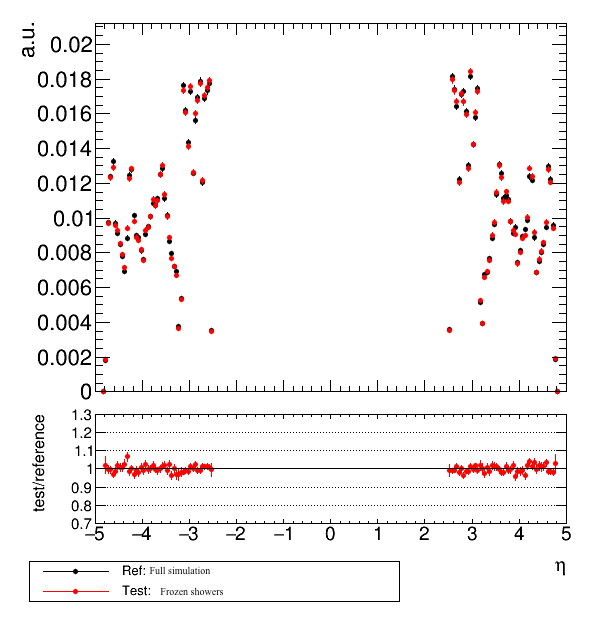
\includegraphics[width=1.\linewidth]{MC/Electron_Frwd_All_KinPlots_eta.png} \\ a)}
\end{minipage}
\hfill
\begin{minipage}[h]{0.49\linewidth}
\center{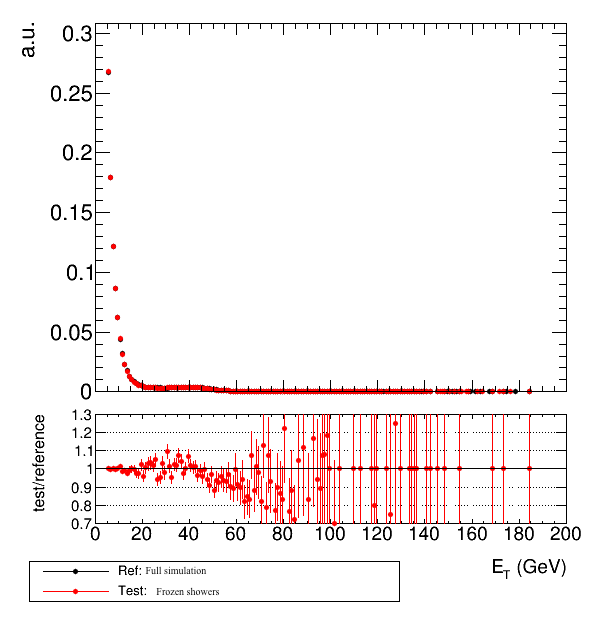
\includegraphics[width=1.\linewidth]{MC/Electron_Frwd_All_KinPlots_et.png} \\ b)}
\end{minipage}
\caption{Results of validation of the frozen showers library on forward electrons. Comparison between full simulation and fast simulation using frozen showers in forward electron events  for a) pseudorapditity and b) electron transverse energy  distributions. Modified from \cite{ElecForwardVal}. }
\label{fig:OtherValFwd}
\end{figure}

\begin{figure}[!tbp]
\begin{minipage}[h]{0.49\linewidth}
\center{\includegraphics[width=1.\linewidth]{MC/Zee_FWDZee_ZMassFWDTight.png} \\ a)}
\end{minipage}
\hfill
\begin{minipage}[h]{0.49\linewidth}
\center{\includegraphics[width=1.\linewidth]{MC/erhResponseVsEta.png} \\ b)}
\end{minipage}
\caption{ Results of validation of the frozen showers library on jets and $Z \to ee$ sample. Comparison between full simulation and fast simulation using frozen showers for and a) mass of the dilepton pair in $Z \to ee$ events (modified from \cite{ZeeVal}) b) jets responce vs  pseudorapditity  distribution (modified from \cite{JetsVal}) . }
\label{fig:OtherVal}
\end{figure}
